	%% Based on a TeXnicCenter-Template by Tino Weinkauf.
%%%%%%%%%%%%%%%%%%%%%%%%%%%%%%%%%%%%%%%%%%%%%%%%%%%%%%%%%%%%%

%%%%%%%%%%%%%%%%%%%%%%%%%%%%%%%%%%%%%%%%%%%%%%%%%%%%%%%%%%%%%
%% HEADER
%%%%%%%%%%%%%%%%%%%%%%%%%%%%%%%%%%%%%%%%%%%%%%%%%%%%%%%%%%%%%

\documentclass[a4paper,12pt]{report}

\usepackage[left=2cm,right=2cm,top=2cm,bottom=2cm]{geometry}
%\usepackage[square,numbers,sort&compress]{natbib}

%% Language %%%%%%%%%%%%%%%%%%%%%%%%%%%%%%%%%%%%%%%%%%%%%%%%%
\usepackage[greek,french]{babel} %francais, polish, spanish, ...
\usepackage[T1]{fontenc}
\usepackage[UTF8]{inputenc}
\usepackage{upgreek} % Permet d'avoir des lettres grecs non italiques
%\usepackage{lmodern} %Type1-font for non-english texts and characters
%\usepackage{sectsty}% Pour changer la taille des chapitres
\usepackage{enumitem}
\usepackage{stmaryrd } % fancy arrow
\usepackage{hyperref}
\hypersetup{
    colorlinks=true,
    urlcolor=theme,
    citecolor=theme
}
\setcounter{tocdepth}{1} %Just show section title in toc
\setcounter{secnumdepth}{3} %add subsubsection numbering in report mode

\usepackage{eurosym}

%% Bibliography Packages %%%%%%%%%%%%%%%%%%%%%%%%%%%%%%%%%%%%%%%%%%%%
\bibliographystyle{template/custom-bib/thesis}
%\bibliographystyle{apalike}
%\bibliographystyle{abbrv}
%\bibliographystyle{alpha}
\usepackage{bibentry}
%\usepackage{multibbl}

%% Figure Packages %%%%%%%%%%%%%%%%%%%%%%%%%%%%%%%%%%%%%%%%%%%%
\usepackage{graphicx} %%For loading graphic files
%\usepackage{subfig}
\usepackage{tabularx} % Permet d'utiliser l'environnement tabularx
%\usepackage{calc} % Pour pouvoir donner des formules dans les définitions de longueur
\usepackage{epstopdf} % à combiner avec la commande pdflatex -shell-escape
\usepackage[export]{adjustbox}

%% Table Packages %%%%%%%%%%%%%%%%%%%%%%%%%%%%%%%%%%%%%%%%%%%%
\usepackage{array,multirow,makecell}

%% Math Packages %%%%%%%%%%%%%%%%%%%%%%%%%%%%%%%%%%%%%%%%%%%%
\usepackage{amsmath}
\usepackage{amsthm}
\usepackage{amsfonts}
\usepackage{amssymb}
\usepackage[thinspace,thinqspace,amssymb]{SIunits}

%% Other Packages %%%%%%%%%%%%%%%%%%%%%%%%%%%%%%%%%%%%%%%%%%%
\usepackage{changepage}   % for the adjustwidth environment

%%%%%%%%%%%%%%%%%%%%%%%%%%%%%%%%%%%%%%%%%%%%%%%%%%%%%%%%%%%%
%% New environnement difinitions
%%%%%%%%%%%%%%%%%%%%%%%%%%%%%%%%%%%%%%%%%%%%%%%%%%%%%%%%%%%%
%\usepackage[colorinlistoftodos,prependcaption,textsize=footnotesize,textwidth=3.0cm]{todonotes}

%\newcommand{\note}[1]{\todo[color=red!15]{#1}}

\usepackage{xcolor}
\usepackage[framemethod=tikz]{mdframed}
\usepackage{chngcntr}

%% Colors %%%%%%%%%%%%%%%%%%%%%%%%%%%%%%%%%%%%%%%%%%%

\definecolor{brun}{rgb}{0.87,0.72,0.53}
\definecolor{brunfonce}{rgb}{0.8,0.4,0.2}
\definecolor{chamois}{rgb}{1.0,0.90,0.70}
\definecolor{bleu_f}{rgb}{0.1,0.1,0.53}
\definecolor{bleu_c}{rgb}{0.8,0.8,0.95}
\definecolor{red_f}{rgb}{0.53,0.1,0.1}
\definecolor{red_c}{rgb}{0.95,0.8,0.8}
\definecolor{green_f}{rgb}{0.1,0.53,0.1}
\definecolor{green_c}{rgb}{0.8,0.95,0.8}
\definecolor{gray_f}{rgb}{0.5,0.5,0.5}
\definecolor{gray_c}{rgb}{0.95,0.95,0.95}
\definecolor{theme}{RGB}{56,115,179}
\definecolor{yellow_f}{rgb}{255,255,0}
\definecolor{yellow_c}{rgb}{255,255,50}

%% Colors new attempts %%%%%%%%%%%%%%%%%%%%%%%%%%%%%%%%%%%%%%%%%%%

\definecolor{gray_f}{RGB}{68,84,106}
\definecolor{gray_c}{RGB}{214,220,229}
\definecolor{bleu_f}{RGB}{91,155,213}
\definecolor{bleu_c}{RGB}{222,235,247}
\definecolor{red_f}{RGB}{204,0,0}
\definecolor{red_c}{RGB}{245,204,204}
\definecolor{orange_f}{RGB}{237,125,49}
\definecolor{orange_c}{RGB}{251,229,214}
\definecolor{green_f}{RGB}{112,173,71}
\definecolor{green_c}{RGB}{226,240,217}
\definecolor{yellow_f}{RGB}{255,192,0}
\definecolor{yellow_c}{RGB}{255,242,204}


%%%%%%%%%%%%%%%%%%%%%%%%%%%%%%%%%%%%%%%%%%%%%%%%%%%%%%%%%%%%%%%%%%%%%%%%
% New environnements
%%%%%%%%%%%%%%%%%%%%%%%%%%%%%%%%%%%%%
% Entete niveau/messsage/prérequis
\newcommand{\niveau}{\textcolor{gray_f}{\textbf{Niveau :}}}
\newcommand{\prerequis}{\textcolor{gray_f}{\textbf{Prérequis :}}}
\newcommand{\objectif}{\textcolor{gray_f}{\textbf{Objectif de la leçon : }}}

%%%%%%%%%%%%%%%%%%%%%%%%%%%%%%%%%%%%%
% Header

\mdfdefinestyle{s_head}{%
	linecolor=gray_f!,
	outerlinewidth=3pt,%
	frametitlerule=false,
	topline=false,
	bottomline=false,
	rightline=false,
	backgroundcolor=gray_c,
	innertopmargin=8pt,
	roundcorner=0pt,
	nobreak=true,
	fontcolor=gray_f
}
\newmdenv[style=s_head]{header_env}
\newenvironment{header}
{%\stepcounter{exa}%
	\addcontentsline{ldf}{figure}{0}%
	\begin{header_env}}
	{\end{header_env}}

%%%%%%%%%%%%%%%%%%%%%%%%%%%%%%%%%%%%%
% Transition

\mdfdefinestyle{s_trans}{%
	linecolor=yellow_f!,
	outerlinewidth=3pt,%
	frametitlerule=false,
	topline=false,
	bottomline=false,
	rightline=false,
	backgroundcolor=yellow_c,
	innertopmargin=8pt,
	roundcorner=0pt,
	nobreak=true
}
\newmdenv[style=s_trans]{transition2_env}
\newenvironment{transition}
{%\stepcounter{exa}%
	\addcontentsline{ldf}{figure}{0}%
	\begin{transition2_env}}
	{\end{transition2_env}}

%%%%%%%%%%%%%%%%%%%%%%%%%%%%%%%%%%%%%
% Experience

\mdfdefinestyle{s_experience}{%
	linecolor=bleu_f!,
	outerlinewidth=3pt,%
	frametitlerule=false,
	topline=false,
	bottomline=false,
	rightline=false,
	backgroundcolor=bleu_c,
	innertopmargin=8pt,
	roundcorner=0pt,
	nobreak=true
}
\newmdenv[style=s_experience]{experience_env}
\newenvironment{experience}
{%\stepcounter{exa}%
	\addcontentsline{ldf}{figure}{0}%
	\begin{experience_env}}
%	\begin{experience_env}[]{\noindent\colorbox[rgb]{0.1 0.1 0.53}{\textbf{\color{white} Expérience : }}\\}}
	{\end{experience_env}}

%%%%%%%%%%%%%%%%%%%%%%%%%%%%%%%%%%%%%
% Slide

\mdfdefinestyle{s_slide}{%
	linecolor=green_f!,
	outerlinewidth=3pt,%
	frametitlerule=false,
	topline=false,
	bottomline=false,
	rightline=false,
	backgroundcolor=green_c,
	innertopmargin=8pt,
	roundcorner=0pt,
	nobreak=true
}
\newmdenv[style=s_slide]{slide_env}

\newenvironment{slide}
	{%\stepcounter{exa}%
%		\newenvironment{myenv}{\begin{adjustwidth}{2cm}{}}{\end{adjustwidth}}
		\addcontentsline{ldf}{figure}{0}%
		\begin{slide_env}}
		{\end{slide_env}
	}

%%%%%%%%%%%%%%%%%%%%%%%%%%%%%%%%%%%%%
% Remarques


\mdfdefinestyle{s_remarque}{%
	linecolor=red_f!,
	outerlinewidth=3pt,%
	frametitlerule=false,
	topline=false,
	bottomline=false,
	rightline=false,
	backgroundcolor=red_c,
	innertopmargin=8pt,
	roundcorner=0pt,
	nobreak=true
}
\newmdenv[style=s_remarque]{remarque_env}
\newenvironment{remarque}
{%\stepcounter{exa}%
	\addcontentsline{ldf}{figure}{0}%
	\begin{remarque_env}\small}
	{\end{remarque_env}
	}
	
%%%%%%%%%%%%%%%%%%%%%%%%%%%%%%%%%%%%%
% Funfacts


\mdfdefinestyle{s_funfact}{%
	linecolor=orange_f!,
	outerlinewidth=3pt,%
	frametitlerule=false,
	topline=false,
	bottomline=false,
	rightline=false,
	backgroundcolor=orange_c,
	innertopmargin=8pt,
	roundcorner=0pt,
	nobreak=true
}
\newmdenv[style=s_funfact]{funfact_env}
\newenvironment{funfact}
{%\stepcounter{exa}%
	\addcontentsline{ldf}{figure}{0}%
	\begin{funfact_env}\small}
	{\end{funfact_env}
	}

%%%%%%%%%%%%%%%%%%%%%%%%%%%%%%%%%%%%%
% Commandes personnelles

\renewcommand{\d}{\mathrm{d}}
\newcommand{\D}{\mathrm{D}}
\newcommand{\sinc}{\mathrm{sinc}}
\newcommand{\grad}{\overrightarrow{\mathrm{grad}}}
\newcommand{\rot}{\overrightarrow{\mathrm{rot}}}
\renewcommand{\div}{\mathrm{div}}

%\renewcommand{\textbullet}{\textcolor{gray_f}{\textbullet}}


%\usepackage[sectionbib]{chapterbib}
%%%%%%%%%%%%%%%%%%%%%%%%%%%%%%%%%%%%%%%%%%%%%%%%%%%%%%%%%%%%
%% DOCUMENT
%%%%%%%%%%%%%%%%%%%%%%%%%%%%%%%%%%%%%%%%%%%%%%%%%%%%%%%%%%%%%
\begin{document}

%\chapter{Leçons de physique} \newpage

\section{LP01 Gravitation}

\begin{header}
\begin{tabular}{p{0.4\textwidth} l}
\niveau & \prerequis \\
CPGE & \textbullet{} Cinématique du point \\
     & \textbullet{} Théorèmes de la dynamique \\
     & \textbullet{} Électrostatique.
\end{tabular}

\noindent
\objectif
Formaliser l'interaction gravitationnelle et étudier le mouvement d'une particule massique dans un champ de pesanteur. 
\end{header}

{
\subsubsection*{Bibliographie}
\footnotesize{}
\begin{itemize}
\item Page Wikipedia sur la \href{https://fr.wikipedia.org/wiki/Constante_gravitationnelle}{constante gravitationnelle} pour la mesure de $G$ ;
\item \cite{Michel2017} chapitre 13
\item \cite{Faroux1996}
\item \cite{Salamito2016}
\item \cite{Bocquet2002}
\end{itemize}
}

\begin{remarque}
Revoir \cite{Michel2017} p472 pour des rappels d'odg sur le système solaire.
Pour ce qui est du niveau : plutôt première année sauf l'analogie avec l'électrostatique qui ne peut être réalisée qu'en deuxième année.
\end{remarque}

\subsection*{Introduction}

La gravitation décrit l'interaction entre des objets de masse non nulle.
Il s'agit d'une des quatre interactions fondamentales.
\begin{slide}
\textbf{Les quatre interactions fondamentales.}
\end{slide}
Elle est de loin la plus faible mais régit l'évolution des astres, ce qui s'explique par la neutralité de la matière et la longue portée des interactions considérées.

Plusieurs modèles des interactions gravitationnelles dans le but d'expliquer le mouvement des objets massifs et notamment celui des astres.
\begin{slide}
\textbf{Plusieurs théories de la gravitation.}
Dire que la théorie de Newton marche très bien dans le cas des masses faibles (incluant le Soleil, ou presque !).
\end{slide}

\begin{transition}
Nous allons décrire dans un premier l'interaction gravitationnelle dans le cadre de la mécanique newtonienne.
\end{transition}

\subsection{Interaction gravitationnelle}

\subsubsection{Force et énergie}

Justifier la forme de l'interaction proposée par Newton \cite{Faroux1996} p146.
Décrire la force gravitationnelle \cite{Michel2017} p337 et \cite{Salamito2016} p569 : à distance, point d'application, attractive, expression.
Principe des actions réciproques.
Parler de $G$ : valeur et mesure \cite{Faroux1996} p148.
Introduire le champ gravitationnel \cite{Salamito2016} p569.

Faire apparaitre l'énergie potentielle gravitationnelle en calculant le travail de la force gravitationnelle \cite{Salamito2016} p622.
Définition d'une force concervative.

\begin{transition}
On remarque une grande similitude entre la force gravitationnelle et l'interaction coulombienne.
Peut-on faire un parallèle entre la gravitation et l'électrostatique ?
\end{transition}

\subsubsection{Champ gravitationnel}

Dresser le parallèle entre la gravitation et l'électrostatique :
\begin{itemize}
\item écrire les forces;
\item montrer les quantités analogues ($m \leftrightarrow q$, $1/4\pi\varepsilon_0 \leftrightarrow -G$);
\item analogie entre ${\cal{G}}$ et $E$.
\end{itemize}
\begin{remarque}
Attention au signe moins devant $G$ ! 
\end{remarque}

Écrire le théorème de Gauss gravitationnel \cite{Faroux1996} p149.
Calculer le champ pour une distribution sphérique de masse volumique uniforme et la tracer en insistant sur les symétries.
Insister sur le fait qu'en dehors de la sphère tout se passe comme si toute la masse était concentrée sur le centre de la sphère.
Théorème de superposition.
Faire l'application numérique pour retrouver l'accélération de pesanteur terrestre.
\begin{remarque}
Le rotationnel de $\overrightarrow{\cal{G}}$ étant nul, on peut aussi définir un potentiel gravitationnel pour le calcul de l'énergie gravitationnelle.
\end{remarque}

Limites du parallèle :
\begin{itemize}
\item force toujours attractive ;
\item pas de masse négative ;
\item pas de champ magnétogravitationnel (en fait si mais compliqué~\cite{Mashhoon2007}, mentionner les ondes gravitationnelles).
\end{itemize}

\begin{transition}
Et le poids dans tout ça ?
Manifestation quotidienne de la gravité.
\end{transition}

\subsubsection{Le poids}

Dire que le poids résulte de la force gravitationnelle et de la force centrifuge (moins de 1\%).

Application de la gravimétrie pour trouver du pétrole etc.

\begin{experience}
\textbf{Mesure de $g$ d'après la période d'oscillation d'un pendule simple.}
Lors des TP de préparation, faire le calcul avec le pendule pesant pour voir si ça améliore la sensibilité.
Plusieurs façons de d'exprimer $T$ : $\sqrt{l/g}$, Borda, intégration.
On pourrait aussi mesurer l'accélération d'une masse en chute libre par analyse d'une vidéo.
\end{experience}

\begin{slide}
\textbf{La Terre homogène ?}
L'unité du graphe est le gal où $\unit{1}{gal} = \unit{1}{\centi\meter\per\second\squared}$.
L'échelle de couleur donne une variation de \unit{100}{\milli gal}, soit $\unit{10^{-3}}{\meter\per\second\squared}$.
\end{slide}

\begin{transition}
Historiquement, les lois de la gravitation ont été établies pour expliquer les observations astronomiques concernant le mouvement des astres dans le système solaire.
\end{transition}

\subsection{Mouvement dans un champ gravitationnel}

Suivre \cite{Michel2017} à partir de p454.
Objectif : étudier le mouvement d'une particule massique dans un champ de pesanteur
Mentionner les trois lois de Kepler et formuler la première : \cite{Michel2017} p460.
On va vérifier cette loi et les autres.

\subsubsection{Position du problème}

On s'intéresse plus particulièrement au mouvement d'une masse ponctuelle autour d'une autre beaucoup plus massive (Terre-Soleil par exemple : le Soleil est fixe).
Position du problème :
\begin{itemize}
\item justifier l'approximation de masse ponctuelle;
\item faire un schéma ;
\item référentiel \cite{Salamito2016} p562 ;
\item bilan des forces, pas de frottements ;
\item PFD et montrer la conservation de la quantité de mouvement du barycentre ;
\item un mot sur le mobile fictif pour la généralisation du problème.
\end{itemize}

C'est un mouvement à force centrale dans un champ newtonien (en $1/r^2$).

\begin{remarque}
L'obtention de l'équation de la trajectoire elliptique n'est pas au programme en PCSI mais elle l'est en MPSI où ils utilisent explicitement les coniques.
La démonstration passe soit par les formules de Binet avec le changement de variable $u=1/r$ où par l'invariant de Runge-Lenz (cf Tout en un MPSI Dunod).

\noindent
Le mobile fictif n'est plus au programme mais si besoin, il est bien fait dans \cite{Bocquet2002} p128.
\end{remarque}

\begin{transition}
Dans ce cadre, étudions le mouvement d'une particule massique dans un champ de gravité.
\end{transition}

\subsubsection{Conservation du moment cinétique}

Établir la conservation du moment cinétique et en déduire :
\begin{itemize}
\item la planéité du mouvement : dans le plan défini par le vecteur vitesse et la force ce qui justifie l'utilisation de coordonnées polaires ;
\item la constante des aires ;
\item la vitesse aréolaire et donc la loi des aires.
\end{itemize}

Formuler la 2ème loi de Kepler : \og le rayon Soleil-planète balaie des aires égales pendant des intervalles de temps égaux \fg{}.

\begin{slide}
\textbf{Vitesse aréolaire.}
Développer le cas circulaire et elliptique et montrer les étoiles au centre de la voie lactée orbitant autour de Sagitarius A : \href{https://www.youtube.com/watch?v=wyuj7-XE8RE}{simulation} ou \href{https://www.youtube.com/watch?v=TF8THY5spmo}{timelapse}.
On l'a illustré dans le cas particulier de trajectoires elliptiques mais c'est aussi valable dans le cas général
\end{slide}

\begin{transition}
La forme des trajectoires est-elle toujours elliptique ?
\end{transition}

\subsubsection{Conservation de l'énergie}

Introduire le potentiel effectif en éliminant $\dot{\theta}$ avec la constante des aires et le tracer en faisant apparaitre les deux contributions.
Problème à un ddl \cite{Bocquet2002} p124.

Faire apparaitre les trois régimes avec le nom des trajectoires.
Retour sur la première loi de Kepler qui est un cas particulier.

\begin{transition}
On souhaite connaitre la période des trajectoires fermées.
\end{transition}

\subsubsection{Période du mouvement}

Dans le cas circulaire, établir l'expression de la vitesse de l'orbite et donner la période du mouvement.
Faire l'application numérique avec la station spatiale internationale et les dires de Thomas Pesquier ($T=\unit{92{,}69}{min}$, cf notebook).

Généraliser aux trajectoires elliptiques pour donner et donner la troisième loi de Kepler \cite{Michel2017} p463.

\begin{slide}
\textbf{Vérification de la troisième loi de Kepler.}
\end{slide}

\begin{transition}
Nous avons bien retrouvé les loi empiriques de Kepler avec l'interaction gravitationnelle proposée par Einstein.
Voyons quelques cas particuliers
\end{transition}

\subsection{Applications et limite}

Toujours dans \cite{Michel2017}.

\subsubsection{Vitesses cosmiques}

Surtout parler de la vitesse de libération et évoquer les trous noirs.

Vitesse de libération sur terre : \unit{11}{\kilo\meter\per\second}.

\subsubsection{Orbite géostationnaire}

Faire les calculs après avoir fait le raisonnement pour montrer qu'elle est unique.
Il y a actuellement environ 300 satellites sur l'orbite, soit un tous les \unit{900}{\kilo\meter}.

\subsubsection{Vers des masses non-ponctuelles}

\cite{Sanz2016} p212 pour la non verticalité de $\overrightarrow{g}$.

Effets de marée, synchronisation des orbites, etc.

\subsection*{Conclusion}

La dernière section peut largement être mise en conclusion si le temps vient à manquer...

On peut remarquer l'équivalence entre masse grave et masse inerte, curiosité de la mécanique newtonienne mais postulat de la RG.
Ouvrir sur la RG avec le retour sur le cas de Mercure dans l'article d'Einstein \cite{Faroux1996} p165.

\begin{remarque}
\href{https://fr.wikipedia.org/wiki/Point_de_Lagrange}{\textbf{Points de Lagrange :}} dans un système à deux corps orbitant l'un autour de l'autre, les cinq points de Lagrange correspondent à des positions où la force centripète due aux deux objets massifs permet à un troisième de masse négligeable de rester fixe par rapport aux deux premiers.
Il y en a deux stables $L_4$ et $L_5$, les trois autres sont instables et généralement occupés par des satellite artificiels.
eLISA sera positionné sur le point $L_1$ du système Terre-Soleil.
\end{remarque}

\begin{funfact}
À propos des travaux d'\href{https://fr.wikipedia.org/wiki/Urbain_Le_Verrier}{Urbain Le Verrier}, astronome et mathématicien français spécialisé en mécanique céleste.
Le 31 août 1846, il annonce l'existence, donne les propriétés et la position de Neptune d'après l'étude des irrégularités de l'orbite d'Uranus.
François Arago dira \og M. Le Verrier vit le nouvel astre au bout de sa plume \fg{}. 
Cette découverte est confirmée par Johann Gottfried Galle le 23 septembre de la même année qui observe le ciel dans la direction des prédictions de Le Verrier.
Plus tard il tente d'expliquer l'anomalie de l'orbite de Mercure par l'existence d'une autre planète, Vulcain, qui ne sera jamais confirmée : il faudra attendre la RG pour donner l'explication appropriée.
\end{funfact}

\newpage
\section{LP02 Lois de conservation en dynamique}

\begin{header}
\begin{tabular}{p{0.4\textwidth} l}
\niveau & \prerequis \\
Template& \textbullet{} Template \\
        & \textbullet{} Template \\
\end{tabular}

\noindent
\objectif
Template
\end{header}

{
%\footnotesize{}
\begin{itemize}
\item \cite{Landau1969} Chapitre II 
\end{itemize}
}

\subsection*{Introduction}

\subsection{Template}

\subsubsection{Template}

\begin{experience}
\textbf{Template}
\end{experience}

\begin{slide}
\textbf{Template}
\end{slide}

\begin{transition}
\textbf{Template}
\end{transition}

\begin{remarque}
\textbf{Template}
\end{remarque}

\newpage
\section{LP03 Notion de viscosité d'un fluide. Écoulement visqueux}

\begin{header}
\begin{tabular}{p{0.4\textwidth} l}
\niveau & \prerequis \\
Template& \textbullet{} Template \\
        & \textbullet{} Template \\
\end{tabular}

\noindent
\objectif
Template
\end{header}

{
%\footnotesize{\bibliography{biblio}}
\bibentry{Template}
}

\subsection*{Introduction}

\subsection{Template}

\subsubsection{Template}

\begin{experience}
\textbf{Template}
\end{experience}

\begin{slide}
\textbf{Template}
\end{slide}

\begin{transition}
\textbf{Template}
\end{transition}

\begin{remarque}
\textbf{Template}
\end{remarque}

\newpage
\section{LP04 Modèle de l'écoulement parfait d'un fluide}

\begin{header}
\begin{tabular}{p{0.4\textwidth} l}
\niveau & \prerequis \\
CPGE & \textbullet{} Statique et dynamique des fluides  \\
     & \textbullet{} Viscosité \\
\end{tabular}

\noindent
\objectif
Mettre en évidence les limites du modèle de l'écoulement parfait et voir quelques applications.
\end{header}

{
\subsection*{Bibliographie}
\footnotesize{}
\begin{itemize}
\item \cite{Olivier2000}
\item \cite{Sanz2016}
\item \cite{Landau1971}
\item \cite{Rabaud2019}
\item \cite{Guyon2001}
\end{itemize}
}

\begin{remarque}
Avoir en tête les principaux effets susceptibles d'être décrits dans ce modèle : Coanda, Magnus, Venturi, portance, etc.
\end{remarque}

\subsection*{Introduction}

L'équation de Navier-Stokes est difficile à résoudre analytiquement :
\begin{itemize}
\item terme d'accélération convective non linéaire ;
\item terme diffusif du second ordre.
\end{itemize}
Dans le cas des écoulement parfaits, l'équation se simplifie.
Écrire l'équation et souligner les termes. 

\subsection{Cadre et limites du modèle}

\subsubsection{Équation d'Euler}


Définition d'un écoulement parfait : \cite{Olivier2000} p432 et \cite{Sanz2016} p311.
Parler de l'évolution isentropique et des grands Reynolds.
Mentionner le cas des ondes acoustiques qui se fait précisément dans ce cadre.

Faire la différence avec les fluides parfait comme l'hélium superfluide \cite{Guyon2001} p170 et p353-355.

Écrire l'équation d'Euler \cite{Sanz2016} p355 et \cite{Olivier2000} p449 sous ses deux formes.
Commentaires

Éventuellement, parler des écoulements particuliers \cite{Sanz2016} p356-357.

\begin{transition}
Pour résoudre l'équation, il est nécessaire de préciser les conditions aux limites.
\end{transition}

\subsubsection{Conditions aux limites}

Il n'y a plus de contrainte tangentielle et les seules forces surfaciques sont les forces de pression.

\begin{slide}
\textbf{Conditions aux limites.}
Le faire par comparaison aux écoulements visqueux.
\end{slide}

\begin{transition}
L'écoulement parfait est un modèle qui possède ses limites.
\end{transition}

\subsubsection{Couche limite}

Suivre \cite{Olivier2000} p433-435 :
\begin{itemize}
\item écoulement parfait : n'existe pas ;
\item notion de couche limite : écoulement parfait en dehors ;
\item épaisseur de la couche limite, limiter la trainée ;
\item raccordement de la vitesse tangentielle ;
\item ordre de grandeur \cite{Sanz2016} p310.
\end{itemize}

\begin{remarque}
La couche limite fait l'objet du chapitre 9 de \cite{Guyon2001}.
\end{remarque}

\begin{transition}
L'équation d'Euler présente seulement des dérivées premières : il est possible de l'intégrer pour trouver des quantités conservées.
\end{transition}

\subsection{Théorème de Bernoulli}

\subsubsection{Équation de conservation de l'énergie}

On néglige les processus dissipatifs : on va pouvoir exprimer la conservation de l'énergie.
Dans un champs de pensanteur uniforme, dans un rférentiel galiléen, établir l'expression du théorème de Bernoulli dans le cas d'un écoulement parfait (on part d'Euler), stationnaire (indépendant du temps), incompressible et homogène ($\rho$ constante) en intégrant le long d'une ligne de courant \cite{Olivier2000} p454.

Interprétation des différents termes : énergie cinétique, énergie potentielle de pesanteur, énergie due au travail des forces de pression.
Voir \cite{Rabaud2019} pour les noms des différents termes, charge, etc.
Évoquer le cas où l'on néglige les effets de la pesanteur et les \og vases énergétiques communicants\fg{}.

\begin{remarque}
Avoir en tête les autres expressions, notamment la version non stationnaire irrotationnel avec le potentiel des vitesses \cite{Olivier2000} p455.
\end{remarque}

\begin{transition}
Voyons quelques applications.
\end{transition}

\subsubsection{Application au tube de Pitot}

Suivre \cite{Rabaud2019} p53 et \cite{Olivier2000} p459.

\begin{slide}
\textbf{Tube de Pitot.}
\end{slide}

\begin{remarque}
Valable seulement si le fluide est incompressible donc un écoulement incompressible : \cite{Guyon2001} p139 pour la condition d'incompressibilité.
\end{remarque}

\begin{experience}
\textbf{Mesure de la vitesse d'un fluide avec un tube de Pitot.}
Comparer les vitesses obtenues avec l'anémomètre et le tube dans la soufflerie.
\end{experience}

\begin{transition}
Le tube de Pitot est utilisé en aviation.
\end{transition}

\subsubsection{Application : l'effet Venturi}

Adapter en fonction du temps : ne pas faire cette partie pour concerver du temps pour la dernière si nécessaire.

Dégager de cette partie qu'une augmentation de la vitesse du fluide se traduit par une diminution de sa pression.

Bien faire le schéma et préciser les hypothèses conformément à précédemment.
Faire le calcul \cite{Olivier2000} p457 et parler du débitmètre.

\begin{experience}
\textbf{Souffler entre deux feuilles pour les rapprocher.}
\end{experience}

\begin{slide}
\textbf{Effet Venturi.}
\end{slide}

Applications : parfums, trompe à eau, artériosclérose.

\begin{transition}
Une mesure différentielle de pression pour mesurer la vitesse : le tube de Pitot.
\end{transition}

\subsection{Écoulement autour d'une aile}

\subsubsection{Écoulement autour d'un obstacle}

Ne pas faire l'analyse quantitative mais elle est faite dans \cite{Olivier2000} p405.

\begin{slide}
\textbf{Écoulement autour d'un obstacle.}
\end{slide}

Raisonner qualitativement et montrer qu'il n'y a pas de portance.
Un des moyens est de faire tourner l'objet : effet Magnus et montrer la \href{https://youtu.be/05zF0sBwHe8?t=85}{vidéo}.

\begin{transition}
L'idée est donc d'avoir une circulation de la vitesse non nulle autour de l'aile.
\end{transition}

\subsubsection{Estimation de la portance}

Suivre \cite{Rabaud2019} p59.

\begin{remarque}
Le calcul analytique est possible (\cite{Olivier2000} p461) mais reste lourd.
Il passe par l'utilisation du potentiel des vitesses dans l'hypothèse d'un écoulement irrotationnel. 
\end{remarque}

\begin{slide}
\textbf{Écoulement autour d'un obstacle.}
\end{slide}

\subsubsection{Paradoxe de d'Alembert}

\cite{Rabaud2019} pour l'énoncé du paradoxe et \cite{Guyon2001} p535-537 pour la levée du paradoxe.

\begin{remarque}
Avoir en tête les problèmes liés au décollement de la couche limite \cite{Guyon2001} p538-543.
\end{remarque}

\subsection*{Conclusion}

Le modèle de l'écoulement parfait permet de simplifier les calculs pour analyser des écoulements loin d'obstacles.
Les effets liés à la viscosité du fluide sont souvent restreints à une faible épaisseur mais qui explique la trainée et la vorticité.

\newpage
\section{LP05 Phénomènes interfaciaux impliquant des liquides}

\begin{header}
\begin{tabular}{p{0.4\textwidth} l}
\niveau & \prerequis \\
Licence & \textbullet{} Statique des fluides \\
        & \textbullet{} Potentiels thermodynamiques \\
        & \textbullet{} Interactions moléculaires
\end{tabular}

\noindent
\objectif
Décrire la tension superficielle et voir ses conséquences sur des interfaces statiques et dynamiques.
\end{header}

{
\subsection*{Bibliographie}
\footnotesize{}
\begin{itemize}
\item \cite{Rabaud2019}
\item \cite{Diu2008}
\item \cite{Marchand2011}
\item \cite{Sanz2016}
\item \cite{Guyon2001}
\item \cite{Graner2011}
\item \cite{Charru2007}
\item \cite{Fruchart2016}
\end{itemize}
}

\begin{remarque}
Pas évident de placer cette leçon au niveau CPGE compte tenu du programme restreint sur cette notion.

\noindent
Rattacher les phénomènes décrits à des observations courantes !
\end{remarque}

\subsection*{Introduction}

Dans la vie courante, et depuis tout petit, on sait qu'il vaut mieux utiliser de l'eau savonneuse pour faire des bulles.
On observe que liquides mouillent différemment les parois solide, qu'il est possible de traiter certaines surfaces pour modifier son comportement par rapport à un fluide.
C'est effet sont liés à la tension de surface que nous allons décrire.

\subsection{La tension de surface}

On modélise l'interface entre deux fluides comme une surface séparant deux fluides...
Dire qu'il s'agit d'un volume dont l'épaisseur est de quelques molécules qui concentre les variation de densité, etc.
Voir la figure 5 de \cite{Marchand2011}.

\subsubsection{Interprétation mécanique}

Suivre \cite{Diu2008} p82-83 pour introduire la tension de surface depuis une expérience.

\begin{experience}
\textbf{Fil tendu par un film de savon.}
\end{experience}

Donner son expression et ses caractéristiques : direction, attractive et unité du coefficient.
Dire que cela ne dépend que de la nature de l'interface.

\begin{experience}
\textbf{Tensiomètre à lame mouillée.}
Passer sur les subtilités dues au mouillage total sur lesquelles on revient plus tard.
\end{experience}

Introduire le travail de la tension superficielle pour la transition.

\begin{transition}
On voit que la tension superficielle est liée à une énergie surfacique.
\end{transition}

\subsubsection{Interprétation thermodynamique}

Bien définir le système et les quantités constantes pour justifier l'emploi de tel potentiel thermodynamique : \cite{Graner2011} p100.
Deux façons de faire :
\begin{itemize}
\item à partir de l'énergie libre dans \cite{Marchand2011} p1 à $T$, $V$ et $n$ fixé ;
\item à partir de l'enthalpie libre dans \cite{Diu2008} p210 dans le cas d'une bulle, à $S$ et $V$ fixés.
\end{itemize}
La deuxième méthode est probablement plus propre mais compliquée à ce stade je trouve.
Dans \cite{Fruchart2016} p473, on donne le potentiel thermodynamique associé à l'étude théorique de la loi de Jurin.

Insister sur l'interprétation : l'augmentation de la surface d'une interface est couteuse en énergie.
Le système tend à minimiser la surface de l'interface.
Dans le cas ou plusieurs interfaces sont susceptibles de se former, la situation d'équilibre est celle d'énergie minimale.

\begin{slide}
\textbf{Surface minimale.}
\end{slide}

\begin{transition}
Poursuivons l'analyse microscopique du phénomène.
\end{transition}

\subsubsection{Interprétation microscopique}

Suivre \cite{Marchand2011} p4-5.
Prendre le temps pour expliquer la figure 6 de l'article.
Donner les ordres de grandeur de la fin de \cite{Marchand2011} p1, avec l'interprétation en terme d'énergie d'interaction dans le liquide.
\begin{slide}
\textbf{Quelques valeurs du coefficient de tension superficielle.}
\end{slide}

Facteurs influençant $\gamma$ :
\begin{itemize}
\item tensioactifs : \cite{Rabaud2019} p81 ;
\item température : \cite{Rabaud2019} p80.
\end{itemize}

\begin{remarque}
Attention à bien justifier que la résultante est parallèle à l'interface.

\noindent
A ce stade, il est normal que l'enthalpie de vaporisation soit liée à $\gamma$ puisque les mêmes interactions microscopiques interviennent.
\end{remarque}

\begin{transition}
Quel est l'effet de la tension superficielle sur l'équilibre des interfaces entre fluides ?
\end{transition}

\subsection{Interface statique}

\subsubsection{Pression}

Retrouver la loi de Laplace avec a force de tension superficielle \cite{Sanz2016} p328.
Citer des exemples pratiques :
\begin{itemize}
\item cohésion du sable mouillé ;
\item retard à l'ébullition \cite{Guyon2001} p57 ;
\item bulle de savon qui se vide dans une plus grande.
\end{itemize}

\begin{remarque}
La formule n'est valable que dans le cas d'une sphère.
Dans le cas général, il faut tenir compte des rayons de courbure dans les deux direction de l'espace normale à l'interface :
\begin{equation}
P_\mathrm{int} - P_\mathrm{ext} = \gamma \left( \frac{1}{R_x} + \frac{1}{R_y} \right).
\end{equation}
Attention aussi au cas de la bulle qui possède deux interfaces.
\end{remarque}

Insister sur l'interprétation qualitative :
\begin{itemize}
\item la surpression est d'autant plus grande que le rayon de courbure est faible ;
\item la pression est plus élevée à l'intérieur de la courbure.
\end{itemize}

\begin{transition}
La tension superficielle permet aussi d'expliquer la capillarité.
\end{transition}

\subsubsection{Capillarité}

Retrouver la loi de Jurin avec l'interprétation énergétique \cite{Sanz2016} p329.

\begin{slide}
\textbf{Loi de Jurin.}
\end{slide}

\begin{experience}
\textbf{Loi de Jurin.}
\end{experience}

\begin{transition}
Utiliser la fin de la slide : la forme de l'interface dépend des coefficients de tension superficielle mis en jeu.
\end{transition}

\subsubsection{Mouillage}

Retrouver la relation de Young-Dupré à partir des deux lois précédentes \cite{Sanz2016} et discuter des différents régimes.

\begin{remarque}
Pour les mesures de l'angle de mouillage, voir \cite{Guyon2001}.

\noindent
Relire \cite{Marchand2011} p7 pour l'interprétation des interactions solide-liquide.
\end{remarque}

\begin{slide}
\textbf{Mouillage.}
\end{slide}

\begin{transition}
Utiliser la fin de la slide avec le mercure pour introduire qualitativement la longueur capillaire.
Elle intervient dans de nombreux phénomènes dynamiques.
\end{transition}

\subsection{Interface dynamique}

\subsubsection{Instabilité de Rayleigh-Taylor}

\begin{experience}
\textbf{Bouteille remplie d'eau et tube fin bouché à une extrémité.}
But comprendre pourquoi l'une des situations est stable et pas l'autre.
\end{experience}
Suivre \cite{Guyon2001} p68-70 et \cite{Charru2007} p53-55.
Donner la longueur capillaire de l'eau.

\subsubsection{Ondes capillaires}

\begin{slide}
\textbf{Ondes à la surface d'un fluide.}
Faire l'analyse qualitative du problème avant de commencer pour mettre en évidence la compétition entre tension superficielle et gravité.
\end{slide}
Faire apparaitre la longueur capillaire.
Dire que l'on peut mesurer aussi la tension superficielle en mesurant cette relation de dispersion.


\subsection*{Conclusion}

On a mis en évidence les propriétés et les manifestations de la tension superficielle qui permettent d'expliquer de nombreux phénomènes de la vie courante, mais aussi des phénomènes plus complexes.

\begin{remarque}
Autres méthodes de mesure de la tension superficielle :
\begin{itemize}
\item méthode d'arrachement, ou méthode de DuNoüy : avec un anneau ;
\item méthode de la goutte pendante ;
\item loi de Jurin ;
\item relation de dispersion des ondes de surface.
\end{itemize}
\end{remarque}

\newpage
\section{LP06 Premier principe de la thermodynamique}

\begin{header}
\begin{tabular}{p{0.4\textwidth} l}
\niveau & \prerequis \\
CPGE & \textbullet{} Modèle du gaz parfait \\
     & \textbullet{} Travail, transfert thermique \\
     & \textbullet{} Transformation thermodynamique \\
\end{tabular}

\noindent
\objectif
Template
\end{header}

{
\subsubsection*{Bibliographie}
\footnotesize{}
\begin{itemize}
\item \cite{Michel2017}
\item \cite{Olivier1998}
\item \cite{Salamito2016}
\item \cite{Diu2008}
\end{itemize}
}

\begin{remarque}
Relire le début de \cite{Diu2008} sur le postulat fondamental de la thermodynamique et p18 pour les variables d'état et équation d'état.
Un mot sur les fonctions d'état p66 et p143.
\end{remarque}

\subsection*{Introduction}

Partir du problème de la conservation de l'énergie mécanique avec l'exemple du livre lancé sur la table \cite{Salamito2016} p905 : ou va l'énergie ?
L'énergie mécanique n'est pas conservée mais l'énergie totale du système l'est.
L'augmentation de la température marque une augmentation de l'énergie microscopique que l'on va chercher à décrire dans cette leçon.

\subsection{Le premier principe}

\begin{remarque}
Équivalence travail-chaleur montrée par Joule en 1843.
Énoncé du premier principe par Mayer en 1845.
\end{remarque}

\subsubsection{Énoncé}

Exprimer la variation de l'énergie totale d'un système pour faire apparaitre l'énergie interne
\begin{equation}
\Delta E_c^\mathrm{macro} + \Delta E_p^\mathrm{macro} + \Delta U = W_\mathrm{nc}^\mathrm{ext} + Q.
\end{equation}
Relire la note de bas de page de \cite{Olivier1998} p132 pour expliquer qu'on suppose $W_\mathrm{nc}^\mathrm{micro} = 0$.
Revenir sur l'exemple introductif.

Se mettre dans le cadre du programme : pas de variation d'énergie potentielle et énergie interne extensive.
Restreindre au cas courant : $\Delta E_c^\mathrm{macro}=0$ et $W_\mathrm{nc}^\mathrm{ext}$ est le travail des forces de pression.
Marquer la différence entre les termes de gauche qui sont des fonctions d'état et les termes de droite qui dépendent du chemin suivi \cite{Michel2017} p533 puis passer à la forme infinitésimale.
\begin{remarque}
L'énergie interne n'est extensive que si les interactions à longue portée sont inexistante ou négligeable : c'est strictement vrai pour le gaz parfait mais pas dans les autres cas.
On peut penser à la tension superficielle notamment, qui est toujours négligée.
\end{remarque}

Insister sur la convention : travail et transfert thermique REÇU par le système comptés positivement.

\begin{transition}
L'énergie interne résulte essentiellement de l'agitation thermique : on souhaiterait relier $U$ et $T$.
\end{transition}

\subsubsection{Capacité calorifique}

Suivre \cite{Salamito2016} p839 et première loi de Joule p841.
Détailler le cas du GP et du solide (loi de Dulong et Petit 1819)

\begin{remarque}
Pour expliquer que $C_V$ soit définit à volume constant : on cherche à expliquer la variation d'énergie interne causée par un $\delta Q$ seulement.
Il faut donc annuler le travail des forces de pression en travaillant à volume constant.
De même pour $C_P$, on souhaite connaitre la variation d'enthalpie causée par un transfert thermique.

\noindent
Le modèle d'Einstein permet d'expliquer la dépendance en température de la capacité calorifique mais il est remplacé par le modèle de Debye pour expliquer la variation aux basses températures.
\end{remarque}

\begin{transition}
Appliquons le premier principe dans le cas de quelques transformations classiques.
\end{transition}

\subsection{Quelques transformations}

\subsubsection{Détente de Joule Gay-Lussac}

\begin{slide}
\textbf{Détente de Joule Gay-Lussac.}
\end{slide}

Suivre \cite{Michel2017} p547.
Bien poser les hypothèses avant de partir dans le calcul.

\begin{remarque}
Si l'on fait l'expérience, on voit que juste après l'ouverture de la vanne, le gaz du récipient initialement plein se refroidit et celui du récipient vide se réchauffe.
En effet le gaz du récipient plein subit une détente adiabatique et celui du récipient vide subit une compression adiabatique.
Après retour à l'équilibre, la température est bien identique à la température initiale.
\end{remarque}

Dans le cas du gaz parfait, il n'y a pas d'élévation de la température ce ui peut servir à savoir si un gaz peut être considéré comme un GP.

\begin{remarque}
Relire l'exercice suivant sur la détente de Joule Thomson au cas où.
\end{remarque}

\begin{transition}
On ressent un échauffement lors du gonflage d'un pneu : peut-on l'expliquer avec le premier principe ?
\end{transition}

\subsubsection{Compression adiabatique}

Suivre \cite{Salamito2016} p903 sur le principe, mais sans force de frottement et en posant une masse $m$ de \unit{5}{\kilo\gram} sur un piston de surface $s=\unit{1}{\centi\meter\squared}$.
On trouve
\begin{equation}
T_f = T_i \frac{5P_0+2P_f}{7P_0} = \unit{729}{\kelvin},
\end{equation}
où $P_f = P_0+mg/s$ et $T_0=\unit{300}{\kelvin}$.

\begin{slide}
\textbf{\href{https://youtu.be/4qe1Ueifekg?t=146}{Fire syringe.}}
\end{slide}

À partir de cet état final, on laisse évoluer (isobare) le système qui va se refroidir en raison d'un transfert thermique $Q$.
Faire apparaitre :
\begin{equation}
\Delta(U+PV) = Q.
\end{equation}

\begin{transition}
Dans une évolution monobare ou isobare, la quantité $U+PV$ est conservée...
\end{transition}

\subsection{Enthalpie}

\subsubsection{Définition}

Suivre \cite{Salamito2016} p906.
Donner la définition et l'unité.
Il peut y avoir d'autres travaux que celui des forces de pression qu'il faut prendre en compte.

Introduire la capacité calorifique à pression constante et la donner pour un GP diatomique, relation de Mayer.
Donner le cas des phases condensées et justifier que $C_P = C_V$ par leur incompressibilité.

\begin{transition}
L'enthalpie se prête particulièrement à la calorimétrie comme nous allons le voir.
\end{transition}

\subsubsection{Calorimétrie}

Présenter le principe \cite{Salamito2016} p915 :
\begin{itemize}
\item vase Dewar : limite les transferts thermiques de conduction et radiatifs ;
\item couvercle percé : peu de convection mais expérience monobare ;
\item agitateur pour l'équilibre ;
\item thermomètre car c'est le seul instrument nécessaire.
\end{itemize}
Principe de la mesure de capacité thermique \cite{Salamito2016} p916.

\begin{remarque}
Ne pas oublier que le calorimètre est un composant du système : il faut prendre en compte sa capacité thermique ou la négliger sous les bonnes approximations.
\end{remarque}

\begin{transition}
Une application importante de la calorimétrie est la détermination des enthalpies de changement d'état.
\end{transition}

\subsubsection{Enthalpie de changement d'état}

Suivre \cite{Salamito2016} p917 et adapter au cas de présent.

\begin{experience}
\textbf{Enthalpie de vaporisation de l'azote liquide.}
\end{experience}

\subsection*{Conclusion}

L'expérience commune montre que les transferts thermiques se font du corps le plus chaud vers le corps le plus froids : deuxième principe.
Il est nécessaire pour comprendre le fonctionnement des machines thermiques.

\subsection*{Questions (FD)}

\begin{enumerate}
\item L'énergie est toujours conservée en physique : ça vient d'où ? Postulé en mécanique newtonienne et démontrable en mécanique lagrangienne par l'intermédiaire du théorème de Noether.
\item Quelle est l'énergie de l'Univers ?
\item Qu'est ce qu'une fonction d'état ? C'est une fonction de variables d'état qui définissent l'état d'équilibre d'un système. Pour une transformation, elle ne dépend pas du chemin suivi.
\item Questions autour de variable/fonction d'état.
\item Qu'est ce qu'une variable extensive ?
\item Est ce que l'énergie interne est toujours extensive ? Non, il faut aussi que les interactions entre les particules du système soient à courte portée.
\item Qu'est ce qu'une transformation ? Passage d'un état d'équilibre à l'autre.
\item Qu'est ce qu'un état d'équilibre ? Équilibre thermique, mécanique et chimique.
\item Quelle est l'énergie cinétique et l'énergie potentielle du premier principe ? Énergie macroscopique du centre de masse
\end{enumerate}

\newpage
\section{LP07 Transitions de phase}

\begin{header}
\begin{tabular}{p{0.4\textwidth} l}
\niveau & \prerequis \\
Template& \textbullet{} Template \\
        & \textbullet{} Template \\
\end{tabular}

\noindent
\objectif
Template
\end{header}

{
%\footnotesize{\bibliography{biblio}}
\bibentry{Template}
}

\subsection*{Introduction}

\subsection{Template}

\subsubsection{Template}

\begin{experience}
\textbf{Template}
\end{experience}

\begin{slide}
\textbf{Template}
\end{slide}

\begin{transition}
\textbf{Template}
\end{transition}

\begin{remarque}
\textbf{Template}
\end{remarque}

\newpage
\section{LP08 Phénomènes de transport}

\begin{header}
\begin{tabular}{p{0.4\textwidth} l}
\niveau & \prerequis \\
CPGE & \textbullet{} Hydrodynamique : notion de viscosité \\
     & \textbullet{} Thermodynamique à l'équilibre \\
     & \textbullet{} Électromagnétisme : loi d'ohm locale, de Joule \\
\end{tabular}

\noindent
\objectif
Template
\end{header}

{
\subsubsection*{Bibliographie}
\footnotesize{}
\begin{itemize}
\item \cite{Olivier1998}
\item \cite{Olivier2000}
\item \cite{Sanz2016}
\item \cite{Guyon2001}
\item \cite{Augier2014}
\item \cite{Taillet2018}
\item \cite{Diu2008}
\end{itemize}
}

\begin{remarque}
En l'état, la leçon est probablement un peu catalogue, ce qui va à l'encontre des retours de jury.
On parle ici majoritairement de diffusion, mais ce n'est pas une leçon sur la diffusion.
Le programme de CPGE ne permet pat d'aller beaucoup plus loin.
\end{remarque}

\begin{experience}
On peut réaliser des expériences qualitatives :
\begin{itemize}
\item diffusion d'une goutte d'encre sur un buvard humide ;
\item simulations de marche aléatoire pour la modélisation microscopique de la diffusion de particules ;
\end{itemize}
et quantitatives :
\begin{itemize}
\item mesure du coefficient de diffusion du glycérol dans l'eau (TP Fluides - Capilarité ;
\item conductivité thermique d'un barreau de cuivre (TP Métaux).
\end{itemize}
\end{experience}

\subsection*{Introduction}

Jusqu'à présent en thermodynamique, on s'est intéressé à des systèmes à l'équilibre auxquels on pouvait associer des grandeurs intensives telles que la température ou la pression.
Le détail des transformations est souvent difficile à étudier car elles peuvent passer par à des systèmes hors équilibres, dans lesquels il existe des transport de plusieurs quantités.
L'étude de ces phénomènes de transport ne ce restreint pas à la thermodynamique :
\begin{itemize}
\item mécanique des fluides : transport de quantité de mouvement ;
\item thermodynamique : transport d'énergie et de particules ;
\item électromagnétisme : transport de charge.
\end{itemize}

L'idée générale est décrite dans \cite{Diu2008} p461 ou l'on étudie le transport de quantités conservées.

\subsection{Généralités}

On va principalement étudier les phénomènes de transport dans le cadre de la thermodynamique tout en établissant les similitudes à d'autres domaines.
Il faut étudier les phénomènes de transport si le système n'est pas à l'équilibre.
Cela nécessite de poser quelques hypothèses (linéarité et ETL) que nous allons tout d'abord énoncer.

\begin{transition}
Quels sont les phénomènes de transports que nous pouvons rencontrer ?
\end{transition}

\subsubsection{Différents phénomènes}

Décrit dans \cite{Olivier2000} p342.
\begin{slide}
\textbf{Différents phénomènes de transport.}
Donner quelque exemples \cite{Sanz2016} p89 :
\begin{itemize}
\item diffusion : parfum, thermique, viscosité, conduction électrique ;
\item convection : brassage de l'air, convection forcée ou naturelle ;
\item rayonnement : prendre l'exemple du vase Dewar.
\end{itemize}
\end{slide}

En général il faut considérer tous les phénomènes de transport.
Cependant, si l'un de ces phénomènes est majoritaire, on peut négliger les autres.
Prendre le cas de l'énergie thermique et donner l'expression du vecteur densité de courant surfacique et son unité \cite{Sanz2016} p122.

\begin{remarque}
À ce stade, on ne précise pas s'il s'agit de conduction, de convection ou de rayonnement.
Voir \cite{Sanz2016} p148 exercice 3{.}9 pour les modèles sur les différents phénomènes.
\end{remarque} 

\begin{transition}
Comme les systèmes étudiés ne sont pas à l'équilibre thermodynamique, il faut faire quelques hypothèses pour étudier ces phénomènes avec les outils de la thermodynamique ou de la mécanique des fluides.
\end{transition}

\subsubsection{Équilibre thermodynamique local}

Reprendre les hypothèses sur l'étude des phénomènes de transport énoncées dans \cite{Diu2008} p465 en commençant par l'équilibre thermodynamique local \cite{Diu2008} p462, définition p464 et \cite{Olivier2000} p344 ;

Il faut dégager les différentes échelles de temps et d'espace.
\begin{slide}
\textbf{Différentes échelles spatiales.}
Faire le parallèle avec la mécanique des fluides et la notion de particules de fluide.
\end{slide}

Pour les échelles temporelles, voir \cite{Diu2008} p463.

Faire le bilan énergétique local à 1D en présence de sources de \cite{Sanz2016} et donner l'équivalent 3D.

\begin{transition}
Pour simplifier l'analyse, on se restreint à des situations proches de l'équilibre ce qui mène à la linéarisation des équations. 
\end{transition}

\subsubsection{Linéarité}

Approximation linéaire \cite{Diu2008} p476.

Donner la loi de Fourier ainsi que ses limites \cite{Sanz2016} p130-131 et \cite{Olivier2000} p348.

Aboutir à l'équation de diffusion avec source \cite{Sanz2016} p132.

\begin{transition}
Les deux équations obtenues permettent d'aboutir à une équation rencontrée dans de nombreux domaines de la physique.
\end{transition}

\subsection{Équation de diffusion}

\subsubsection{Analogies}

Donner l'expression de l'équation de diffusion thermique sans source et mettre en évidence
\begin{itemize}
\item la grandeur intensive : $T$ ;
\item la grandeur extensive conservée : $E$ ;
\item l'origine de la diffusion : $\grad$ qui donne lieu à un flux de la quantité conservée.
\end{itemize}
\cite{Diu2008} p479 sur les conditions initiales nécessaires à la résolution de l'équation.

\begin{slide}
\textbf{Équation de diffusion.}
Bien relire \cite{Olivier2000} p361-363 et marquer les limites de l'analogie.
Pour la viscosité, on se place dans le cas de l'écoulement de Couette plan.

\noindent
Donner un exemple pour chaque situation :
\begin{itemize}
\item barreau de cuivre ;
\item fibre à gradient d'indice, \cite{Olivier1998} p92 ;
\item mise en évidence du caractère diffusif de la viscosité \cite{Olivier2000} p444 ;
\item conduction électrique dans un conducteur.
\end{itemize}
\end{slide}

\begin{slide}
\textbf{Ordres de grandeur.}
Continuer sur les limites de l'analogie en montrant les différences qui peuvent être énormes entre les ordres de grandeur.
En revanche, on remarque la proximité des coefficients de diffusion dans les gaz : c'est normal car le même processus microscopique est à l'œuvre : \cite{Olivier2000} p428.
\end{slide}

Donner la loi d'échelle qui lie temps caractéristique, taille caractéristique et coefficient de diffusion comme \cite{Olivier2000} p354 et \cite{Diu2008} p480.

\begin{remarque}
Davantage de détails sur la loi de Fick dans \cite{Diu2008} p477, sur la loi d'Ohm p483 et sur le transport de quantité de mouvement p514.

\noindent
Être conscient que dans les deux cas, le gradient à l'origine du transport porte en toute rigueur sur le potentiel chimique.
De manière générale, l'inhomogénéité d'une grandeur se traduit par un flux de la grandeur thermodynamique conjuguée \cite{Diu2008} p524.

\noindent
L'effet de peau obéit à une équation de diffusion \cite{Olivier2000} p765-766.
\end{remarque}

\begin{transition}
Cette équation générale décrit un phénomène irréversible : on le voit directement car elle fait intervenir une dérivée première par rapport au temps.
Un interprétation microscopique permet de comprendre pourquoi.
\end{transition}

\subsubsection{Caractère irréversible}

Remarque générale de \cite{Olivier2000} et lire \cite{Diu2008} p480.

Bien poser le cadre : étude d'un gaz monoatomique sans mouvement macroscopique ce qui permet de considérer uniquement la diffusion.

\begin{slide}
\textbf{Diffusion et marche aléatoire.}
\end{slide}

\begin{remarque}
Modèle microscopique de la diffusion thermique dans un gaz monoatomique dans \cite{Olivier2000} p351 et de la viscosité p426.

\noindent
On peut montrer le caractère irréversible de la diffusion thermique en faisant un bilan d'entropie \cite{Sanz2016} p134.
\end{remarque}

\begin{remarque}
Attention à l'équation de Schrödinger : sa forme est celle d'une équation de diffusion mais à coefficient complexe.
Elle est réversible par un changement de $t$ en $-t$ et de $\psi$ en $\psi^\dagger$.
Voir les entrées Schrödinger, rotation de Wick et réversible de \cite{Taillet2018}.
\end{remarque}

\begin{transition}
On peut exploiter les propriétés du phénomène de diffusion pour mesurer la conductivité d'un matériau.
\end{transition}

\subsubsection{Mesure de la conductivité thermique du cuivre}

\begin{experience}
\textbf{Mesure de la conductivité thermique d'un barreau de cuivre.}
Valeurs tabulées : 
\begin{itemize}
\item $\lambda_\mathrm{Cu}=\unit{390\times 10^{-6}}{\watt\cdot\meter^{-1}\cdot\kelvin^{-1}}$ ;
\item $\rho_\mathrm{Cu} = \unit{8{,}93\times10^3}{\kilo\gram\cdot\meter^{-3}}$ ;
\item $c_\mathrm{Cu} = \unit{0{,}382}{\kilo\joule\cdot\kilo\gram^{-1}\cdot\kelvin^{-1}}$ ;
\item $D_\mathrm{Cu} = \unit{117\times10^{-6}}{\meter^2\cdot\second^{-1}}$.  
\end{itemize}
On en déduit un temps caractéristique pour l'établissement du régime permanent de l'ordre de \unit{85}{\second} (pour un barreau de \unit{10}{\centi\meter}).
\end{experience}

Faire un schéma et résoudre l'équation de Laplace.
Les conditions aux limites $T(x=0)=T_0$ et ${\cal{P}}=S\lambda\frac{\partial T}{\partial x}$ donnent :
\begin{equation}
T(x) = \frac{\cal{P}}{S\lambda} x + T_0.
\end{equation}
Comparer la valeur mesurée avec les valeurs tabulées en justifiant l'écart avec le fait que l'intégrale de la puissance électrique fournie à la résistance n'est pas transmise au barreau.
On doit normalement obtenir une conductivité plus grande que prévue.

\begin{remarque}
Avoir en tête la loi de Wiedemann-Franz qui lie la conductivité thermique, électrique et la température (voir \href{http://ressources.agreg.phys.ens.fr/ressources/}{TP Métaux}).
\end{remarque}

\begin{transition}
On l'a vu la diffusion n'est pas le seul moyen de transport.
Comment peut-on les comparer ?
\end{transition}

\subsection{Comparaison entre les différents phénomènes}

\subsubsection{Résistance thermique}

Établir l'expression de la résistance thermique de conduction \cite{Sanz2016} p140, donner la loi de Newton et la résistance associée au rayonnement p148.

\begin{slide}
\textbf{Résistance thermique en régime permanent.}
La résistance associée à la convection est donnée pour un \og jour de grand vent \fg{}.
Donner l'interprétation de cette loi : continuité microscopique sur une couche limite thermique de faible épaisseur qui apparait comme une discontinuité macroscopique \cite{Diu2008} p498.
\end{slide}

\begin{remarque}
Remarques sur le transport convectif de chaleur \cite{Guyon2001} p564.
\end{remarque}

\begin{transition}
Pour expliquer le comportement d'un système, il est souvent suffisant de tenir compte uniquement du phénomène majoritaire.
Comme en mécanique des fluides, on peut distinguer différents régime grâce à des nombres addimensionnés.
\end{transition}

\subsubsection{Phénomène prépondérant}

Exprimer le rapport entre convection en $U \times \rho U$ et diffusion en $\eta \grad U$ et remarquer qu'il s'agit du nombre de Reynolds et revenir sur le rapport entre les termes de l'équation de Navier-Stokes.

Mentionner les nombres de Péclet et Prandtl \cite{Guyon2001} p102-103.
Application numérique pour une tasse et du sucre :
\begin{equation}
Pe = \frac{UL}{D} = \frac{10^{-2}\times 5.10^{-2}}{0,52.10^{-9}} \approx 10^4.
\end{equation}
La diffusion est remarquablement inefficace !

\subsection*{Conclusion}

\begin{slide}
\textbf{Obtention de très basses températures  : un cryostat à dilution.}
Récapituler les différents transferts thermiques qu'il est nécessaire contrôler pour obtenir des température aussi basses. 
\end{slide}

Ouvrir sur l'effet Seebeck, Peltier \cite{Diu2008} p518 et suivantes.

\newpage
\section{LP09 Conversion de puissance électromécanique}

\begin{header}
\begin{tabular}{p{0.4\textwidth} l}
\niveau & \prerequis \\
CPGE (PSI) & \textbullet{} Induction \\
           & \textbullet{} Force de Laplace \\
           & \textbullet{} Énergie électromagnétique \\
           & \textbullet{} Électrocinétique \\
           & \textbullet{} Notion de couple, puissance mécanique
\end{tabular}

\noindent
\objectif
Template
\end{header}

\subsection*{Bibliographie}
{
\footnotesize{}
En gros : Polycopié de Jérémy et Dunod PSI (apparemment la dernière édition est la meilleure)
\begin{itemize}
\item \cite{Faroux1998}
\item \cite{Salamito2016}
\item \cite{Neveu2019}
\item \cite{Cardini2017}
\item \cite{Naval}
\end{itemize}
}

\subsection*{Introduction}

Électricité à la base de notre société : permet de transporter de l'énergie qu'il faut convertir en lumière, chaleur ou travail.
Les moteurs et générateurs sont des exemples de machines tournantes très fréquemment rencontrés depuis la production électrique jusqu'aux moyens de transport.
Ces machines sont constituées d'un stator et d'un rotor (définir).

\subsection{Induction et force de Laplace}

Ne pas faire cette partie probablement par manque de temps et redondance avec le moteur continu.

On peut probablement la faire rapidement mais en insistant lourdement sur la correspondance entre énergie méca et elec.

On s'intéresse à une barre en mouvement dans un champ magnétique uniforme.
On trouve :
\begin{equation}
e = lBv
\end{equation}
Explication physique : l'opérateur met en mouvement les particules chargées du conducteur qui sont déviées par le champ magnétique.
On peut alors assimiler cet effet à une force électromotrice $e$.

La puissance électrique est donnée par 
\begin{equation}
{\mathcal{P}}_e = ilBv
\end{equation}
Ici un déplacement crée une force électromotrice, mais on sait qu'un champ magnétique variable en crée aussi ce qui est important dans les machines électromécaniques : soit un conducteur se déplace dans un champ magnétique soit le champ magnétique est variable.
Faire le schéma équivalent électrique.

Si l'induction transforme l'énergie mécanique en énergie électromagnétique, la force de Laplace fait l'inverse.

Seule la force de Laplace est à prendre en compte :
\begin{equation}
F_L = -ilB
\end{equation}
dont la puissance est
\begin{equation}
{\mathcal{P}}_L = -ilBv
\end{equation}

On montre immédiatement l'égalité entre les puissances d'induction et de Laplace ce qui est l'essentiel de la conversion électromécanique.

\begin{transition}
Il existe des applications ou l'on souhaite faire des translations mais souvent une rotation plus utile.
\end{transition}

\subsection{Machine à courant continu}

\subsubsection{Cas d'une spire -- Laplace}

Suivre le cours de Jérémy

\begin{slide}
\textbf{Modèle de la machine à courant continu.}
\end{slide}

\begin{slide}
\textbf{Couple de la machine à courant continu.}
\end{slide}

\begin{transition}
On a un circuit mobile dans un champs magnétique constant ce qui conduit au phénomène d'induction.
\end{transition}

\subsubsection{Cas d'une spire -- Induction de Lorentz}

Retrouver l'égalité des puissance mécanique (Laplace) et de l'induction en fonction du couple, de la vitesse de rotation, de la force électromotrice et du courant.

\begin{transition}
Le couple d'un tel système n'est pas acceptable, il faut utiliser plusieurs spires et des matériaux ferromagnétiques pour optimiser le couplage entre les champs rotoriques et statoriques.
\end{transition}


\subsubsection{Généralisation aux machines réelles}

\begin{slide}
\textbf{Machine à courant continu réelle}
\end{slide}

Introduire la constante de couplage électromécanique et établir l'expression de la vitesse de rotation en fonction de la force contre électromotrice.
Insister sur le fait qu'ils sont facilement contrôlables (vitesse, piles).

\begin{experience}
\textbf{Caractérisque $\omega(E)$ du moteur à courant continu.}
\end{experience}

Dire un mot sur la réversibilité de ces machine mais sera développé après.

\begin{transition}
Ces machines sont essentielles mais présentent des inconvénients :
\begin{itemize}
\item pour la production : le transport d'électricité en CC n'est pas rentable, il vaut mieux utiliser le triphasé.
\item pour les moteurs : contacts glissants qui s'abîment, puissances modérées. 
\end{itemize}
\end{transition}

\subsubsection{Machine synchrone}

Avant on avit un moment magnétique variable dans un champ magnétique permanent, maintenant on va voir un moment magnétique constant dans un champ magnétique variable

\subsubsection{Création d'un champ tournant}
\label{sec:lp09_rotating_field}

Faire le cas avec un champ diphasé pour avoir l'idée puis montrer le cas réel avec 3 bobines.

\begin{slide}
\textbf{Création d'un champ tournant.}
\end{slide}

En plaçant un dipôle au centre, celui-ci sera soumis à un couple qui peut le mettre en rotation.

\begin{experience}
\textbf{Boussole dans un champ magnétique tournant.}
\end{experience}

\begin{transition}
En pratique les champs obtenu grâce à de simples spires n'est pas très intense et il faut utiliser un milieux ferromagnétique doux pour canaliser le champ magnétique.
\end{transition}

\subsubsection{Champ statorique}

\begin{slide}
\textbf{Modèle de la machine synchrone.}
Parler des hypothèses et insister sur le rôle du matériau ferromagnétique.
\end{slide}

\begin{slide}
\textbf{Champ statorique.}
\end{slide}

Calculer le champs statorique avec le théorème d'Ampère dans les milieux comme dans le bouquin de PSI en faisant attention à bien justifier les symétries, etc.

Aboutir sur l'expression du champ glissant (la donner par analogie avec la partie~\ref{sec:lp09_rotating_field} si manque de temps).

Donner l'expression du champ rotorique par analogie avec le cas d'une seule spire.

\subsection{Couple de la machine synchrone}

Suivre le livre de PSI pour déterminer l'expression de l'énergie électromagnétique dans l'entrefer et en déduire l'expression du couple.
Faire apparaitre la condition de synchronisme puis discuter des différents régimes de fonctionnement. 

\begin{slide}
\textbf{Caractéristique $\Gamma(\alpha)$}
\end{slide}

Faire un bilan de puissance comme dans le poly de Jérémy et insister sur les conventions.

Discuter des avantages et inconvénients de la machine synchrone (ouvrir sur les problèmes liés au démarrage et éventuellement montrer la cage d'écureuil)

\subsection*{Conclusion}

\newpage
\section{LP10 Induction électromagnétique}

\begin{header}
\begin{tabular}{p{0.4\textwidth} l}
\niveau & \prerequis \\
Licence & \textbullet{} Electrocinétique \\
        & \textbullet{} Forces de Laplace \\
        & \textbullet{} Equations de Maxwell \\
        & \textbullet{} Potentiels \\
\end{tabular}

\noindent
\objectif
Comprendre l'origine physique de l'induction et quantifier ses effets. Les illustrer à travers plusieurs applications.
\end{header}

{
%\footnotesize{}
\subsection*{Bibliographie}
\begin{itemize}
\item \cite{Perez2009}
\item \cite{Sanz2016}
\item \cite{Neveu2019a}
\item \cite{Bertin1984}
\end{itemize}
}

\begin{remarque}
Dans cette leçon, il faut faire particulièrement attention à insister sur l'importance du choix des conventions d'orientation et les respecter.
L'introduction de la fem d'induction est délicate : avoir en tête les différentes approches possibles (empirique, modèle de Drude et force de Lorentz, changement de référentiel) et être prêt à défendre ses choix.
Les aspects énergétiques sont importants.
\end{remarque}


\subsection*{Introduction}

Qu'est ce que l'induction ?

\begin{experience}
En approchant un aimant d'une bobine, on constate l'apparition d'un courant.
C'est l'induction : à partir d'un champ $\overrightarrow{B}$ on peut créer un courant dans un conducteur.
\end{experience}

\begin{slide}
Expérience historique de Faraday (1831) dans laquelle il observe le courant dans une bobine créé par une autre bobine alimentée par une pile.
Il pensait que le courant été créé par un champ magnétique, mais c'est en allumant la bobine qu'on observe effectivement un courant : il faut une variation du champ $\overrightarrow{B}$.
\end{slide}

\begin{experience}
On observe l'apparition de courant quand l'aimant se déplace dans la bobine. En revanche, il n'y a pas de courant quand $\overrightarrow{B}$ est statique.
\end{experience}

\begin{transition}
On va essayer de quantifier cet effet.
\end{transition}

\subsection{Les lois de l'induction}

\subsubsection{La loi de Faraday 2'30}

Relire le début du poly de Jérémy sur les moteurs pour l'introduction de la fem.

Dans le cadre de l'ARQS, on s'intéresse à un contour fermé $ABCD$ placé dans un champ magnétique $\overrightarrow{B}$ et on donne une vitesse $\overrightarrow{v}$ au circuit.
On calcule la force de Lorentz qui s'applique aux porteurs de charge du circuit
\begin{equation}
\overrightarrow{F} = q(\overrightarrow{E} + \overrightarrow{v}\wedge\overrightarrow{B}).
\end{equation}
La démonstration est faite dans \cite{Perez2009}.
On en déduit la force électromotrice qui correspond au travail de la force de Lorentz divisé par $q$.
On utilise les potentiels scalaire et vecteur pour réécrire $E$.
Le terme en $\grad V$ est nul car le contour fermé.
Avec le théorème de Stokes-Ampère, on transforme l'intégrale sur $\d\overrightarrow{A}/\d t$...
En intégrant sur tout le circuit, on obtient finalement
\begin{equation}
e=-\iint \frac{\partial\overrightarrow{B}}{\partial t}\d \overrightarrow{S} + \int (\overrightarrow{v}\wedge\overrightarrow{B})\overrightarrow{\d l}
\end{equation}

Cette expression fait apparaitre les deux termes de l'induction :
\begin{itemize}
\item Neumann, associé à une variation temporelle de $\overrightarrow{B}$ ;
\item Lorentz, associé à un déplacement du circuit dans un champ magnétique non uniforme.
\end{itemize}

Dans le cas d'un circuit indéformable, on retrouve la loi de Faraday, qui fait intervenir la dérivée totale du flux :
\begin{equation}
e = - \frac{\D \Phi}{\D t}
\end{equation}

Plutôt que d'établir cette formule il est sans doute préférable d'étudier les cas particuliers utiles pour la leçon :
\begin{itemize}
\item induction de Neumann : se contenter d'un circuit fixe et indéformable dant un champ magnétique variable.
Eventuellement parler des flux coupé pour la généralisation de cette loi qui est la loi empirique.
Insister sur la convention d'orientation.
\item induction de Lorentz : garder le terme $\overrightarrow{v}\wedge\overrightarrow{B}$.
\end{itemize}

\begin{transition}
Le signe moins de la loi de Faraday est très important.
Il indique que l'induction va créer un courant dont le sens s'oppose à sa cause (le champ magnétique créé par ce courant tend à s'opposer à la variation de flux qui lui donne naissance).
C'est la loi de modération de Lenz.
\end{transition}

\subsubsection{Loi de Lenz 10'}

Les effets de l'induction s'opposent à la cause qui les a produit.

Cette loi qualitative permet de prévoir les effets de l'induction.

\begin{experience}
Chute d'un aimant dans différent tubes
\begin{itemize}
\item tube en plexiglas : c'est un isolant, il n'y a pas d'induction, l'aimant tombe rapidement sous l'effet de la gravité ;
\item tube en cuivre : c'est un bon conducteur, le courant créé dans le tube par l'aimant qui tombe génère un champ magnétique qui ralenti l'aimant.
C'est une manifestation de la loi de Lenz.
\end{itemize}  puis cuivre.
\end{experience}

Pendant la leçon, penser à traiter qualitativement les cas étudiés avec la loi de Lenz.

\begin{transition}
Maintenant que l'on a étudié les aspects théoriques de l'induction, on va étudier chacun des deux régimes.
Commençons par l'induction de Neumann (champ $\overrightarrow{B}$ variable).
\end{transition}

\subsection{Induction de Neumann (B variable) 12'}

\subsubsection{Auto-induction}

%\begin{figure}[!h]
%\center
%\includegraphics[scale=1]{Lecons_de_physique_2019-2020/Lecons_autres/bobine.png}
%\end{figure}

Importance de l'agébrisation : l'orientation du courant défini l'orientation des surfaces.
On calcule le flux propre dans le cas où l'on suppose que le champs$\overrightarrow{B}$ créé par la bobine est celui d'un solénoide infini.
Le calcul du flux à travers une spire, puis $N$ spires donne
\begin{equation}
\Phi_B = \frac{\mu_0 N^2 S i}{l}
\end{equation}
En appliquant la loi de Faraday, on trouve
\begin{equation}
e = -L\frac{\d i}{\d t},
\end{equation}
où $L = \mu_0 N^2 S/l$ est l'inductance de la bobine  
$L$ s'exprime en Henri ($\mathrm{H}=\meter^2\cdot\kilogram\cdot\second^{-2}\cdot\ampere^{-2})$.

Ici la bobine est traitée en convention générateur car elle est assimilée dans le circuit à un générateur.
En convention récepteur, on a l'habitude de travailler avec $U_L = -e$.
(Schémas au tableau des deux circuits dans chacune des deux conventions, avec la bobine et une résistance $R$ en série.)

L'énergie stockée dans la bobine est liée à son inductance et se trouve en exprimant la puissance électrique qui parcourt la bobine :
\begin{equation}
{\cal{E}} = \frac{1}{2}Li^2
\end{equation}

\begin{remarque}
L'énergie stockée dans la bobine se retrouve aussi en calculant l'énergie volumique magnétique $B^2/2\mu_0$ et en multipliant par le volume de la bobine.
\end{remarque}

\begin{experience}
Vérification de la dépendance en $N^2$ de l'inductance de plusieurs bobines en mesurant l'inductance d'après la fonction de transfert d'un circuit RL :
\begin{itemize}
\item mesure de l'inductance de quatre bobines de même géométrie mais avec des nobres de spires différents (125, 250, 500 et 1000 spires).
Une mesure est réalisée devant le jury.
\item il est nécessaire de mesure $R$ à chaque fois car la résistance dépend de la longueur de fil de la bobine. Cette mesure est réalisée précisément à l'aide d'un multimètre Keithley permettant de faire une mesure à quatre points.
\item la mesure de $L$ se fait en déterminant la fréquence de coupure du filtre passe bas du premier ordre $RL$.
Pour cela on mesure le rapport entre la tension $U_R$ et la tension du GBF, et on réalise l'acquisition pour différentes fréquences à l'aide du programme python dédié à la mesure de diagramme de Bode.
\item en ajustant sur Qtiplot la courbe obtenue par le modèle analytique $||H(\omega)|| = \frac{1}{\sqrt{1+(\omega/\omega_c)^2}}$, on en déduit $L$ (connaissant $R$) car $\omega_c = R/L$.
\item les différentes valeurs de $L$ obtenue sont ajustée en fonction du nombre de spire par un modèle $\mu_0N^\alpha S/L$ et on obtient bien $\alpha\approx2$.
\end{itemize}
Comparaison entre les valeurs mesurées et les valeurs déduites de la géométrie des bobines.
\end{experience}

\begin{transition}
Regardons ce qui se passe maintenant dans le cas de l'expérience de Faraday, avec deux bobines.
\end{transition}

\subsubsection{Inductance mutuelle 25'}

Schéma de deux bobines d'inductance $L_1$ et $L_2$, parcourue par des courants $i_1$ et $i_2$.
L'inductance mutuelle traduit le couplage entre les deux circuits :
\begin{equation}
e_2 = -L_2\frac{\d i_2}{\d t} - M\frac{\d i_1}{\d t}
\end{equation}

\begin{remarque}
\begin{itemize}
\item le signe de $M$ dépend de l'orientation des deux circuits ;
\item on montre que $M_{12}$ = $M_{21}$ : le résultat est presque immédiat en passant par le potentiel vecteur (démo dans \cite{Perez2009} par exemple).
\item l'énergie d'un système de deux inductance couplées par une mutuelle est donnée par 
\begin{equation}
E_\mathrm{tot} = \frac{1}{2}L_1 i_1^2 + M i_1 i_2 + \frac{1}{2}L_2 i_2^2
\end{equation}
\end{itemize}
\end{remarque}

L'inductance mutuelle traduit le fait qu'il est possible de transférer de l'énergie d'un circuit à l'autre.

Traiter le cas du transformateur : faire le calcul de $i_1/i_2$ avec le théorème d'Ampère et déduire la relation en tension par conservation des puissances.
Une application importante de cet effet est le transformateur, nécessaire au transport de l'énergie à haute tension pour diminuer les pertes dues au transfert (les pertes par effets Joule sont proportionnelles au carré de l'intensité.
En travaillant avec des tensions très élevées ($\sim \unit{400}{\kilo\volt}$), il est possible de transporter des puissances importantes sans avoir un courant important.
On a $P_J = Ri^2 = U^2/R$, mais le $U$ ici correspond à la différence de potentiel entre les deux extrémités du fil électrique, et pas aux $\unit{400}{\kilo\volt}$ qui est la différence de potentiel entre le cable et la terre.)
Le transformateur est utilisé pour abaisser la tension en vue d'une utilisation par les particuliers.

\begin{transition}
Après l'induction de Neumann, on va s'intéresser à l'induction de Lorentz, c'est à dire à un circuit mobile.
\end{transition}

\subsection{Induction de Lorentz (circuit mobile) 28'30}

\subsubsection{Rail de Laplace}

Deux termes : 
\begin{itemize}
\item force électromotrice : elle traduit le couplage mécanique $\rightarrow$ électrique ;
\item force de Laplace, responsable du couplage électrique $\rightarrow$ mécanique.
\end{itemize}
Schémas du dispositif, mécanique et électrique.

Avant la mise en équation, on peut qualitativement déterminer l'évolution du système lors d'un déplacement de la tige avec la loi de Lenz (...).
Mise en équation :
\begin{itemize}
\item équation électrique
\begin{equation}
Ri = -vlB
\end{equation}
\item équation mécanique : principe fondamental de la dynamique projeté selon x
\begin{equation}
m\dot{v} = ilB
\end{equation}
\end{itemize}
La résolution de ce système donne 
\begin{equation}
v = v_0 e^{-t/\tau}
\end{equation}
où $\tau = \frac{mR}{B^2 l^2}$.
La barre est ralenti, ce qui est en accord avec l'analyse qualitative avec la loi de Lenz.
Si l'on souhaite arrêter complètement la barre, il faut rajouter un frottement mécanique.

Conversion électromécanique :
Schéma des échanges ($P_{laplace}$ et $P_{induction}$) pour faire le lien entre les pertes par effet Joule et la variation d'énergie cinétique.
On a $P_{laplace} + P_{induction} = 0$

\begin{slide}
Freinage par induction utilisé pour les poids lourds ou encore les trains (présente l'avantage de ne pas nécessité de pièce d'usure).
Les courants créés dans la masse métallique sont appelés courants de Foucault.
Une autre application de l'induction de Lorentz est la roue de Barlow qui peut être utilisée comme générateur de générateur de courant continu (actuellement, cette méthode sert encore pour générer les courants intenses nécessaires aux électrolyses).
L'induction est aussi à la base des méthodes de production d'électricité (alternative) actuelles.
\end{slide}

\begin{experience}
Rail de Laplace : le rail a tendance à rester collé sur le support (les faux contacts entre les rails et la tige créent des arcs électriques qui soudent la barre aux rails).
On pourrait ici faire une démonstration qualitative de la roue de Barlow.
\end{experience}

\subsection*{Conclusion 39'}

Au cours de cette leçon, on a vu :
\begin{itemize}
\item les lois de l'induction (Lenz et Lorentz) ;
\item les inductions de Neumann et Lorentz.
\end{itemize}

\begin{slide}
Applications : générateurs, chauffage par induction, micro, chargeur sans fil...
\end{slide}

\begin{slide}
\href{https://www.youtube.com/watch?v=nIFSZfKTUKA}{Railgun de l'espace} pour la blague :)	
\end{slide}


\subsection*{Questions}

\begin{enumerate}
\item Lors de l'approche historique avec l'expérience de Faraday, vous avez parlé de galvanomètre : qu'est-ce que c'est ? Il s'agit d'un instrument permettant de mesurer de faibles courants électriques.
L'aiguille de l'appareil est liée à des spires parcourue par le courant à mesurer, spires placées dans un champ magnétique constant et homogène.
Le dipôle magnétique formé par les spire est alors soumis à un couple qui dévie l'aiguille.
\item Lors de l'introduction des lois de l'induction, vous avez introduit trois ingrédients : force de Lorentz, $\overrightarrow{E} = -\grad V - \d\overrightarrow{A}/\d t$ et $\overrightarrow{v}\wedge\overrightarrow{B}$ : Commenter ces termes. La force de Lorentz permet d'expliquer comment le champ electromagnétique peut mettre en mouvement ou dévier des particules chargées.
On repart des équations de Maxwell pour exprimer $\overrightarrow{E}$ en fonction des potentiels vecteur et scalaire.
\item Que représentent $V$ et $\overrightarrow{A}$ ?
voir le cours d'électromag de Jérémy pour des discussions plus poussées.
On ne peut pas mesurer directement ni l'un ni l'autre.
On a seulement accès à des différences de potentiel ou à la circulation de $\overrightarrow{A}$.
Dans le cas d'un solénoide parfait avec une spire autour, le champ $\overrightarrow{B}$ est nul au niveau de la spire pourtant il est possible de crée un fem dans la spire en faisant varier le courant dans le solénoïde (le champ $\overrightarrow{B}$ est bien nul mais pas $\overrightarrow{A}$ au niveau de la spire).
Une autre expérience mettant en évidence le rôle de $\overrightarrow{A}$ dans la compréhension d'effets subtils est celle d'Aharonov-Bohm.
\item Comment pourrait-on préciser l'introduction de la force électromotrice $e$ ? Lien entre le travail et la ddp (le travail de la force de lorentz permet d'introduire la ddp)
\item Dans la force de Lorentz, Que représente $\overrightarrow{v}$ ? C'est la vitesse des porteurs de charge.
\item Quel est le référentiel dans lequel est défini $\overrightarrow{v}$ ?
\item vitesse du circuit = vitesse des charges ?
Ici il faut utiliser la composition des vitesses :$\overrightarrow{v} = \overrightarrow{v_{circuit}} + \overrightarrow{u}$, où $\overrightarrow{v_{circuit}}$ est la vitesse du circuit dans le référentiel du laboratoire et $\overrightarrow{u}$ est la vitesse des électrons dans le référentiel lié au circuit.
Quand on considère l'effet d'un champ magnétique sur les électrons, on peut alors considérer le cas d'un conducteur filiforme : la vitesse $\overrightarrow{u}$ étant alors toujours colinéaire avec le conducteur, seule la vitesse des électrons liée au mouvement du circuit donne lieux à une circulation non nulle ($\overrightarrow{u}\wedge\overrightarrow{B}$ est toujours orthogonal au conducteur).
Dans le cas d'un conducteur ayant une section finie, le déplacement de électrons le long du circuit donne en présence d'un champ magnétique l'effet Hall qui est négligeable dans les conducteur en raison de la densité importante de porteurs de charge.
\item Comment évolue la vitesse de chute de l'aimant en fonction du matériau du tube ? Plus le matériaux est conducteur, plus le freinage est efficace, donc la chute longue.
\item Justifier l'approximation du solénoïde infini pour les bobines ?
Cette approximation est sans doute discutable car : les bobines utilisées sont de section carrée et la dimension de la section est comparable à la longueur de la bobine.
Cependant, même dans le cas d'une simple spire, le champ créé en dehors de l'axe est compliqué à calculer.
Les résultats obtenus lors des expériences étant en accord raisonnable avec le modèle simple d'un champ uniforme, on peut ici justifier l'utilisation de cette approximation.
\item Pourquoi sommer les champs $\overrightarrow{B}$ ? On peut appliquer le principe de superposition associé à la linéarité des équations de Maxwell.
\item Pourquoi se placer en convention générateur ? Dans le cas de l'induction présenté ici, la bobine est la source de la force électromotrice.
Il s'agit d'un générateur qui justifie l'emploi de la convention associée. 
\item Puissance stockée dans la bobine. Pourquoi $iU_L$ et pas $ei$ ? Lié à la convention choisie : en convention générateur, on considère l'énergie cédée par la bobine au circuit.
En convention récepteur, on s'intéresse à l'énergie reçue par la bobine.
\item Manip : Quelle est la valeur de la résistance de la bobine et justifier le choix de la résistance ?
(dépend du nombre de spires de la bobine) Il faut que la résistance de la bobine reste faible devant la résistance placée en série avec la bobine.
De plus, on fait en sorte que la fréquence de coupure du passe base soit de l'ordre de \unit{10}{\kilo\hertz} 
\item D'où viennent les incertitudes sur la mesure ? Comment sont calculées les erreurs ? Lors de la mesure de la fréquence de coupure, l'incertitude vient de l'ajustement des données expérimentales par le modèle analytique.
La déduction de $L$ dépend aussi de la valeur de la résistance $R + r$ qui est mesurée précisément avec l'ohmmètre numérique et une mesure à quatre points.
Cette incertitude est données par la notice de l'appareil.
\item Est-il possible de rajouter des erreurs sur les points acquis à l'oscilloscope à la main ?
Oui en se référant à la notice de l'instrument mais elles sont petites venant de l'oscilloscope.
\item Pourquoi avoir choisi de mesurer $L$ d'après le diagramme de Bode ?
Essentiellement car il faut une mesure quantitative dans la leçon docteur.
Autres méthodes : umax/2, temps de montée, etc.
Justifiée par une approche pédagogique.
\item Valeur d'inductance comparée à quoi ? A celle mesuré au RLC-mètre, à la valeur annoncée par le constructeur, à la valeur attendue compte tenu du modèle.
\item D'où vient l'incertitude sur l'inductance théorique ? Principalement de l'inhomogénéité du champ $\overrightarrow{B}$ dans toutes les spires et sur toute la surface d'une même spire.
\item Inductance mutuelle ? pourquoi mettre des dérivée ronde ? (erreur)
\item Une seule équation : couplage de 1 vers 2. Qu'est ce qui se passe dans l'autre sens ?
Le problème est symétrique.
\item L'inductance mutuelle est elle la même de 12 ou 21 ? Oui.
\item Équivalence des puissances de Laplace et induit ? Oui car sinon fuck la physique.
\item Roue de Barlow pour générer du courant ? Oui pour les forts courants de certaines électrolyses, non pour la production électrique actuelle (alternateurs).
\end{enumerate}

\subsection*{Commentaires}

Point noir de la leçon : comment amener les lois de l'induction ?
On peut écrire que la vitesse des électrons est la composition des électrons dans le circuit + la vitesse du circuit.
Une autre possibilité serait de faire l'approche historique entière et introduire le dphi directement.
Bq d'applications : bien
A n'est pas mesurable car il y a une jauge près mais ddp mesurable et la circulation de A aussi.
\newpage
\section{LP11 Rétroaction et oscillations}

\begin{header}
\begin{tabular}{p{0.4\textwidth} l}
\niveau & \prerequis \\
CPGE    & \textbullet{} Filtrage linéaire \\
        & \textbullet{} ALI, modèle d'ordre un \\
        & \textbullet{} Fonction de transfert \\
        & \textbullet{} Diagramme de Bode
\end{tabular}

\noindent
\objectif
Template
\end{header}

{
\subsubsection*{Bibliographie}
\footnotesize{}
\begin{itemize}
\item \cite{Neveu2019a}
\item \cite{Cardini2017}
\end{itemize}
}

\begin{remarque}
Le programme est vaste !
Les quatre premiers chapitres de \cite{Cardini2017} rentrent dans le cadre de la leçon.
Elle est franchement orientée PSI.

\noindent
Il faut prendre parti dès le début je pense : justifier rapidement qu'on utilise $p$ à la place de $j\omega$.
Même si on ne le dit pas explicitement pendant la leçon, on se place ainsi dans le formalisme de Laplace et ça simplifie les notations.
Quand on parle de polynôme pour la fonction de transfert, c'est encore plus évident avec $p$ qu'avec un polynôme en $j\omega$.
Garder en tête que contrairement à la transformée de Fourier, la transformation de Laplace fait intervenir les conditions initiales.

\noindent
Il faut poser calmement le schéma bloc du système et identifier $A$ et $\beta$ à chaque fois pour éviter de se mélanger les pinceaux.
Dans le montage amplificateur non inverseur, $A$ est la fonction de transfert de l'ALI, $\beta$ celle du pont diviseur.
Dans l'oscillateur à pont de Wien, $A$ est la fonction de transfert de l'amplificateur non inverseur et $\beta$ celle du filtre de Wien.
Bien faire attention à différencier fonction de transfert en boucle ouverte et boucle fermée !

\noindent
Par rapport au rapport de jury qui précise de différencier système bouclé et rétroaction : un système bouclé a sa sortie reliée à son entrée ce qui est une rétraction particulière.
Dans un système asservi on compare la sortie à l'entrée alors que dans un système bouclé, la sortie est l'entrée.
\end{remarque}

\subsection*{Introduction}

Les rétroactions sont nécessaires pour assurer la stabilité de nombreux systèmes : elles interviennent dans les asservissements : un automobiliste ajuste sa trajectoire afin de ne pas finir dans un platane.
Les perturbations, ici les changements de direction de la route, sont captées visuellement, analysées par le cerveau puis l'action adaptée est envoyée pour corriger la trajectoire.

Toutefois, une rétroaction inappropriée peut mener à une instabilité : par exemple l'effet Larsen.
Cette instabilité est parfois problématique puisqu'elle peut mener à la rupture de tout ou partie du système.
Dans certains cas, la rétroaction mène à une comportement périodique qui, s'il est maitrisé permet de construire des oscillateurs à la base du fonctionnement des montres par exemple.

\begin{slide}
\textbf{Rétroaction et oscillations.}
Apparemment, il y a des concours de Larsen...
\end{slide}

\subsection{Nécessité d'une rétroaction}

\subsubsection{Thermostat}

Décrire le principe de la boucle ouverte et de la boucle fermée avec un exemple pratique, une régulation de température :
\begin{itemize}
\item en boucle ouverte : on donne une consigne à un radiateur qui va permettre de compenser les pertes thermiques dans une pièce.
Si rien ne change, pas de problème mais si la température extérieure évolue, il faudra adapter la consigne.
On ne veut pas ajuster en permanence la consigne donc on va automatiser le système en lui ajoutant une boucle de contrôle.
\item en boucle fermée, la sortie est comparée à la consigne et le système ajuste son action.
\end{itemize}
Faire apparaitre le schéma bloc du système en présentant les protagonistes : consigne, actuateur (radiateur), rétroaction (thermomètre) et comparateur (soustracteur).

\begin{transition}
Ce formalisme est très général et particulièrement adapté à la description des systèmes bouclés.
Appliquons le à un système facilement accessible en TP : le montage amplificateur non inverseur.
\end{transition}

\subsubsection{Amplificateur non inverseur}

On s'intéresse à des systèmes linéaires, continus et invariants \cite{Cardini2017} p31.
Suivre \cite{Neveu2019a} p74 pour introduire la fonction de transfert en boucle ouverte et boucle fermée en prenant pour l'ALI un modèle de passe-bas du premier ordre.
Introduire les notions de chaine directe et chaine de retour \cite{Cardini2017} p47.
Montrer qu'en prenant $\mu_0 \rightarrow \infty$, on retrouve bien un amplificateur.
Il faut être efficace dans les calculs.

\begin{experience}
\textbf{Amplificateur non inverseur.}
Mesurer sa fonction de transfert et la relier aux valeurs des composants.
\end{experience}

Montrer la conservation du produit gain bande et tracer le diagramme de Bode pour quelques gains : il faut souligner que le montage est un passe-bas.
Faire apparaitre clairement le lien avec l'asservissement présenté précédemment et parler de précision et rapidité.
Dire qu'en réalisé on ajoute un correcteur.
De manière très générale, les asservissements sont un compromis entre rapidité, précision et stabilité.

\begin{remarque}
La fonction de transfert harmonique d'un système linéaire est aussi appelée transmittance harmonique.

\noindent
Bien relire \cite{Neveu2019a} p84-88 pour être au clair sur le PID au cas où.

\noindent
Il faut faire la différence entre l'électronique de puissance où la précision n'est pas aussi importante que l'obtention de forts courants et le traitement du signal par exemple où la précision est essentielle pour préserver la fidélité du signal. 
\end{remarque}

\begin{transition}
La présence d'une rétroaction adaptée est essentielle pour les asservissements : amplificateur, thermostat, robotique, etc.
Cependant, elle peut mener à un système instable.
\end{transition}

\subsection{Stabilité}

\subsubsection{Comparateur à hystérésis}

\begin{experience}
\textbf{Comparateur à hystérésis.}
Montrer que l'inversion des bornes amène une saturation du système : la rétroaction peut conduire à une instabilité.
\end{experience}

Analysons ce qu'il se passe \cite{Neveu2019a} p90 :
\begin{itemize}
\item reprendre le modèle du premier ordre de l'ALI pour justifier l'effet de l'inversion du signe : on passe de $\mu_0$ à $-\mu_0$ ;
\item reprendre la fonction de transfert simplifiée de l'amplificateur non inverseur comme un passe-bas d'ordre un et passer en réel pour obtenir l'équation différentielle du filtre ;
\item analyser qualitativement l'effet du changement de signe de $\mu_0$ en remarquant qu'une exponentielle croissante ou décroissante est solution.
\item parler de la saturation qui empêche la divergence du système.
\end{itemize}
On comprend bien pourquoi la rétroaction sur la borne non inverseuse est source d'instabilité.

\begin{transition}
Étudions le cas général.
\end{transition}

\subsubsection{Critère de stabilité}

On se limite en accord avec le programme à des systèmes d'ordre deux :
\begin{itemize}
\item écrire l'équation différentielle générale du système ;
\item donner l'équivalence du critère de stabilité \cite{Cardini2017} p38 et interpréter physiquement le rôle du signe du coefficient d'amortissement.
Donner la condition générale en terme de signe pour les coefficients \cite{Neveu2019a} p91 ;
\item passer en complexe pour écrire la fonction de transfert et bien souligner l'équivalence des deux notations ;
\item définir un système stable \cite{Cardini2017} p35 ;
\item remarquer que l'ordre du numérateur est forcément inférieur à celui du dénominateur sinon divergence à haute fréquence ;
\item la condition de stabilité porte donc sur le dénominateur : remarquer qu'il ne doit pas s'annuler et dire que la limite de stabilité du système est atteinte aux zéros du dénominateur.
\end{itemize}
Deux points importants à retenir :
\begin{itemize}
\item on peut connaitre la stabilité du système en étudiant sa réponse en boucle ouverte, il ne faut pas que $H_\mathrm{TBO}=-1$ ;
\item les descriptions fréquentielle et temporelle sont équivalentes : on étudie souvent la réponse impulsionnelle.
\end{itemize}

\begin{remarque}
La stabilité d'un système fermé est définie avec des marges en gain et en phase car les paramètres de la rétroaction sont susceptibles de changer en raison de variation thermique etc.

\noindent
Le fait que l'ordre du numérateur soit plus faible que celui du dénominateur dans la fonction de transfert traduit aussi la causalité du système \cite{Neveu2019a} p78.

\noindent
Savoir parler du lieu de Nyquist.

\noindent
La réponse temporelle des systèmes linéaires est réalisée en utilisant le formalisme de Laplace : la connaissance de la fonction de transfert et des conditions initiales permet de remonter très simplement à l'évolution temporelle du circuit grâce à une transformation inverse de Laplace.
Ce n'est toutefois pas vraiment au programme de PSI même s'ils passent du $j\omega$ à $p$ dans les calculs.
Il semble que ce soit vu un peu plus en SI.
\end{remarque}

\begin{transition}
Les instabilité sont potentiellement dangereuses mais peuvent être exploitées pour créer des oscillateurs.
\end{transition}

\subsection{Oscillateur quasi sinusoïdal}

\subsubsection{Système bouclé}

Faire le schéma \cite{Neveu2019a} p97 et réécrire les fonctions de transfert en boucles ouverte et fermée en faisant attention au changement de signe dû au passage d'un soustracteur à un sommateur.
Reprendre l'exemple de l'amplificateur non inverseur et dire que c'est débile de le boucler mais que si on ajoute un passe bande, on va pouvoir sélectionner une composante spectrale.
Mettre l'accent sur la condition pour observer une oscillation : gain unitaire et déphasage nul.
Bien faire apparaitre la nécessité d'un amplificateur.
Énoncer la condition de Barkhausen \cite{Neveu2019a} p98.

\begin{transition}
Voyons un exemple pratique, l'oscillateur à pont de Wien.
\end{transition}

\subsubsection{Analyse de la boucle ouverte}

Reprendre l'amplificateur et lui ajouter le filtre de Wien sans boucler, identifier $A$ et $\beta$ et faire le schéma bloc.
Suivant le temps, on fait les calculs ou on balance.

\begin{experience}
\textbf{Filtre de Wien.}
Mettre en évidence qu'à résonance le déphasage est nul.
Résonance au sens réponse maximale mais gain inférieur à un : il faut un ampli.
\end{experience}

Trouver la condition d'oscillation avec le critère de Barkhausen \cite{Neveu2019a} p100.

\begin{experience}
\textbf{Fonction de transfert en boucle ouverte.}
Se rapprocher des conditions d'oscillation en restant en dessous.
\end{experience}

\begin{transition}
Et maintenant, on boucle !
\end{transition}

\subsubsection{Oscillateur à pont de Wien}

\begin{experience}
\textbf{Oscillateur à pont de Wien.}
Bam ! Ça oscille.
On peut regarder le portrait de phase pour vérifier que les oscillations sont presque sinusoïdales.
Mettre en évidence que la saturation est responsable de la non divergence des oscillations : sauvé par la non-linéarité !
\end{experience}

Parler du facteur de qualité : ici c'est nul on a 1/3 mais avec des quartz, on transfert la stabilité mécanique d'un micro-diapason sur un oscillateur électronique.
C'est à la base de tous les appareils électroniques récents.
Applications suivant le temps : montre, laser...

\begin{remarque}
Ici on ne s'intéresse qu'à un type d'oscillateur : l'oscillateur quasi-sinusoïdal mais il existe aussi l'oscillateur à relaxation \cite{Neveu2019a} p103.
\end{remarque}

\subsection*{Conclusion}

En récapitulant, on peut parler des correcteurs sur les asservissements par exemple.
Donner des exemples.

\newpage
\section{LP12 Traitement d'un signal, étude spectrale}

\begin{header}
\begin{tabular}{p{0.4\textwidth} l}
\niveau & \prerequis \\
CPGE (MP, PSI) & \textbullet{} Electrocinétique, fonction de transfert \\
			   & \textbullet{} Filtre RC
\end{tabular}

\noindent
\objectif
Mettre en évidence l'importance du traitement de signal dans les protocoles de communication actuels.
Discuter des avantages et inconvénients des traitements numériques et analogiques.
Se familiariser avec l'étude spectrale.
\end{header}

{
\footnotesize{}
\subsection*{Bibliographie}
\begin{itemize}
\item \cite{Augier2014}
\item \cite{Cardini2017}
\item \cite{Salamito2017}
\item \cite{Neveu2019}
\end{itemize}
}

\begin{remarque}
Cette leçon se prête particulièrement bien à des expériences qualitatives rapides sur l'oscilloscope, aussi bien dans le filtrage avec l'étude de l'action du RC sur un créneau par exemple que pour montrer le traitement numérique.
Il faut bien reprendre en main l'oscilloscope, notamment sur la FFT pour montrer rapidement les effets mentionnés dans la leçon. 
\end{remarque}

\subsection*{Introduction}

Dans le cadre des télécommunications, on s'intéresse à la transmission d'un signal complexe qui doit être traité afin d'être transporté sur de longues distances.
On distingue les méthodes analogiques qui conservent la nature continue du signal des méthodes numériques qui nécessite sa discrétisation.
Ces deux méthodes présentent chacune des avantages et inconvénients que l'on discutera au cours de cette leçon.
L'étude spectrale permet de s'affranchir de la redondance temporelle de la plupart des signaux et constitue donc un outils puissant pour leur étude.

On peut peut-être partir aussi en présentant directement le signal GW150914 bruité et la nécessité du filtrage pour extraire un signal faible d'un bruit important.
Le passage modulation/démodulation est justifié par l'utilisation de ces technique dans l'interféromètre mais aussi sur la détection elle même : l'OG introduit une  modulation de phase qui est détectée par interférométrie (démodulation).

\subsection{Spectre d'un signal et filtrage}

\begin{remarque}
L'objectif de cette partie est de justifier le passage à l'étude de spectre et de comprendre comment agit un système simple (filtre linéaire) sur le signal.
Par la suite il est possible d'étudier directement les spectres.
\end{remarque}

Le signal est une grandeur physique dons les variations temporelles encodent une information.

\subsubsection{Signal périodique}

Suivre \cite{Salamito2017}.
Tout signal périodique $s(t)$ de fréquence $f_s$ s'exprime comme la superposition de fonctions sinusoïdales de fréquence multiple de $f_s$ :
\begin{equation}
s(t) = A_0 + \sum_{n=1}^\infty A_n \cos(2\pi n f_s t + \varphi_n).
\end{equation}
Toutes les informations sur $s(t)$ sont contenues dans les $A_n$ et $\varphi_n$ : on peut les représenter en fonction de la fréquence sous forme de spectres en amplitude et en phase.
Faire les schémas $s(t)$, $A_n(f)$ et $\varphi_n(f)$.

\begin{slide}
\textbf{Spectre d'un signal en créneau.}
\end{slide}

\begin{experience}
\textbf{FFT d'un signal en créneau sur l'oscilloscope.}
\end{experience}

Donner les interprétations physiques de $A_0$, $A_1$ et $A_n$ : les premières harmoniques décrivent la forme générale du signal mais les détails sont donnés par les hautes fréquences, c'est-à-dire par les harmoniques de rang élevé.

\begin{slide}
\textbf{Spectre du signal sonore émis par un verre.}
Parler de la transformée de Fourier pour les signaux non périodiques. 
\end{slide}

\begin{transition}
Cette description permet de s'affranchir de la redondance d'un signal périodique et est particulièrement utile pour décrire la réponse des filtres linéaires.
\end{transition}

\subsubsection{Filtrage linéaire}

\begin{remarque}
Attention à la cohérence dans cette partie avec les pré-requis : si les filtres électroniques ont déjà été vus, il n'est pas utile d'introduire les notions de diagramme de Bode etc.
Il faut plutôt je pense rattacher la description générale au cas particulier des filtres électroniques.
\end{remarque}

Faire une schéma d'un filtre avec $e$ et $s$.
Définition d'un filtre : système pour lequel il existe une relation à coefficients constants entre les dérivées temporelles de l'entrée et celles de la sortie :
\begin{equation}
b_0 s(t) + b_1 \frac{\d s}{\d t} + ... + b_m \frac{\d^m s}{\d t^m} = a_0 e(t) + a_1 \frac{\d e}{\d t}+ ...
\end{equation}
$m$ est appelé l'ordre du filtre.
Ce type de système est linéaire ce qui permet d'utiliser le principe de superposition.
Il permet d'agir sur le spectre d'un signal sans modifier le contenu fréquentiel (ne fait pas apparaitre de nouvelle fréquences, ce qui traduirait une non-linéarité).

On suppose un signal d'entrée de la forme :
\begin{equation}
e(t) = E\cos(\omega t+\varphi_e)
\end{equation}
et on utilise la notation complexe :
\begin{equation}
\underline{e}(t) = E e^{j(\omega t + \varphi_e)}.
\end{equation}
En faisant de même pour la sortie, on définit la fonction de transfert d'un filtre linéaire comme le rapport :
\begin{equation}
\underline{H}(j\omega) = \frac{\underline{s}}{\underline{e}}.
\end{equation}

Calculs du filtre RC en utilisant les impédances complexes.
On obtiendrait le même résultat en établissant l'équation temporelle du circuit.

\begin{slide}
\textbf{Filtre passe-bas.}
\end{slide}

\begin{experience}
\textbf{Diagramme de Bode d'un circuit RC.}
Montrer l'effet du filtre sur un signal sinusoïdal en modifiant la fréquence pour mettre en évidence le caractère passe bas.
Faire les calculs puis acquérir et ajuster le diagramme de Bode obtenu par le modèle.
\end{experience}

\begin{remarque}
Prendre le temps de discuter l'altération du spectre en fonction de la différence de fréquence entre le signal et le filtre dans le cas simple du passe-bas.
\end{remarque}

Mettre en évidence le comportement intégrateur du passe-bas par le calcul dans le cas $\omega\gg\omega_c$ et par l'expérience.

De manière générale les filtres permettent d'isoler une partie du spectre d'un signal pour en extraire l'information essentielle dont la nature varie avec l'application : musique, télécommunications, mesures de précisions...
Il existe de nombreux types de filtres linéaires : passe-bas, passe-haut, passe-bande, etc. et pas seulement d'ordre 1.
Ils peuvent agir dans des domaines différents (mécanique, électronique, etc.).

\begin{transition}
Ces systèmes linéaires sont nécessaires pour le traitement du signal dans les télécommunications mais pas suffisants.
\end{transition}

\subsection{Transmission analogique : la radio AM}

\begin{remarque}
Avantages de la modulation d'amplitude : simplicité, longue portée car basse fréquence.
Inconvénients : sensibles aux perturbations sur l'amplitude.

\noindent
Avantage de la modulation de fréquence : insensible aux perturbations (sauf effet doppler ou non linéarités).
Inconvénient : plus complexe, plus faible portée.
\end{remarque}

\subsubsection{Modulation}

On s'intéresse à la transmission d'une musique pour expliquer le fonctionnement de la radio par exemple.
Il est exclu de les transmettre via des ondes mécaniques pour des raisons évidentes : on préfère utiliser des ondes électromagnétiques.
Il faut donc premièrement transformer le signal sonore en signal électrique grâce à un microphone par exemple.
La fréquence du signal à transmettre est de l'ordre du kHz, ce qui correspond à une longueur d'onde de \unit{300}{\kilo\meter}.
Comme les antennes sont du même ordre de grandeur que le signal à détecter il faudrait des antennes gigantesques !
Pour éviter cela on va utiliser une porteuse de haute fréquence pour transporter l'information base fréquence, ce qui nécessite une modulation.

Cette opération nécessite un composant non linéaire : le multiplieur.
Faire un schéma
\begin{equation}
s_{AM}(t) = (1+\alpha s(t))s_p(t)
\end{equation}
Faire le calcul pour montrer que 
\begin{equation}
s_{AM}(t) = A_p \left[ \cos(\omega_p t) + \frac{m}{2}\cos(\omega_p-\omega)t + \frac{m}{2}\cos(\omega_p+\omega)t \right] 
\end{equation}
On voit immédiatement que le signal modulé contient trois fréquences.

\begin{slide}
\textbf{Spectre du signal modulé en amplitude.}
\end{slide}

Parler du problème de la porteuse qui nécessite beaucoup d'énergie.

\begin{transition}
On obtient donc un signal qui peut être transporté mais qui n'est pas utilisable en tant que tel.
Il est nécessaire de le démoduler.
\end{transition}

\subsubsection{Démodulation synchrone}

Parler rapidement de la détection d'enveloppe.

Faire le calcul de la démodulation synchrone et insister sur l'importance du filtrage.
 
\begin{slide}
\textbf{Spectre du signal démodulé en amplitude.}
\end{slide}

\begin{transition}
Si les télécommunication analogiques sont encore utilisées actuellement, le numérique devient de plus en plus présent.
Inconvénients de la transmissions analogique : sujet au bruit, difficile à stocker.
\end{transition}

\subsection{Traitement numérique}

\subsubsection{Numérisation}

Avantages du numériques \cite{Cardini2017} p136.
Définition de l'échantillonnage \cite{Cardini2017} p127.

\begin{slide}
\textbf{Numérisation d'un signal.}
\end{slide}

Il y a une perte d'information mais facilement mémorisable.

\begin{slide}
\textbf{Critère de Shanon.}
\end{slide}
Parler des DFT, FFT.
Tracer le spectre d'un signal échantillonné et faire apparaitre la création de nouvelle fréquence en raisonnant par analogie avec la modulation vue avant.
Repliement de spectre.
Amener la nécessité de filtrer avant l'acquisition pour éviter le repliement de spectre.

\begin{transition}
\textbf{Template}
\end{transition}

\subsubsection{Filtrage}

Présenter la méthode de discrétisation en prenant l'exemple du passe bas.

\begin{slide}
\textbf{Filtrage numérique.}
\end{slide}

Le traitement du signal peut être fait a posteriori mais aussi en temps réel : parler des micro-contrôleurs qui permettent de réaliser des filtres complexes sans modifier le hardware.
Il y a donc plus de flexibilité !

\subsection*{Conclusion}

\begin{slide}
\textbf{Traitement du signal pour la détection des ondes gravitationnelles.}
Il faut garder du temps pour traiter convenablement cette partie : elle permet de récapituler le contenu de la leçon :
\begin{itemize}
\item étude d'un spectre ;
\item filtrage analogique : expliquer les systèmes de suspension des miroirs filtrage passe-bande pour éliminer hautes et basses fréquence du signal à la sortie de l'interféromètre ;
\item filtrage numérique : traitement du signal pour éliminer les harmoniques, analyse des données (massives) et automatique.
\end{itemize}
\end{slide}

On peut aussi parler des asservissements.

\newpage
\section{LP13 Ondes progressives, ondes stationnaires}

\begin{header}
\begin{tabular}{p{0.4\textwidth} l}
\niveau & \prerequis \\
Template& \textbullet{} Template \\
        & \textbullet{} Template \\
\end{tabular}

\noindent
\objectif
Template
\end{header}

{
\subsubsection*{Bibliographie}
\footnotesize{}
%\begin{itemize}
%\item 
%\end{itemize}
}


\subsection*{Introduction}

\subsection{Template}

\subsubsection{Template}

\begin{experience}
\textbf{Template}
\end{experience}

\begin{slide}
\textbf{Template}
\end{slide}

\begin{transition}
\textbf{Template}
\end{transition}

\begin{remarque}
\textbf{Template}
\end{remarque}

\newpage
\section{LP14 Ondes acoustiques}

\begin{header}
\begin{tabular}{p{0.4\textwidth} l}
\niveau & \prerequis \\
CPGE    & \textbullet{} Mécanique des fluides \\
        & \textbullet{} Thermodynamique \\
        & \textbullet{} Ondes électromagnétiques \\
\end{tabular}

\noindent
\objectif
Décrire les ondes acoustiques dans différents milieux, leur propagation et ainsi expliquer le principe de fonctionnement de plusieurs instruments de musique. 
\end{header}


\subsection*{Bibliographie}
{
\footnotesize{}
\begin{itemize}
\item \cite{Chaigne2008}
\item \cite{Brebec2004}
\item \cite{Morse1986}
\item \cite{Sanz2016}
\item \cite{Landau}
\item \cite{Metzdorff2017}
\item \cite{Stanford2014}
\end{itemize}
}

\subsection*{Introduction}

Montrer l'extrait de la vidéo~\cite{Stanford2014}.
Dans cette vidéo, on a vu de nombreux exemples qui montrent le caractère vibratoire des ondes acoustiques et leur lien avec le son, la musique.
L'objectif de cette leçon va être de décrire les ondes acoustiques, principalement dans les fluides et de voir comment leur manipulation peut conduire à la fabrication d'instruments, mais aussi à la compréhension du comportement de nombreux objets.

\subsection{Description d'une onde acoustique}

Les ondes acoustiques sont des ondes mécaniques.
Elles correspondent à la propagation d'une déformation dans un milieu matériel.
Insister sur la nécessité d'un milieu matériel, qui peut être fluide ou solide.
Ici on va principalement s'intéresser aux ondes acoustiques dans l'air.

\subsubsection{Approximation acoustique}

Les ondes acoustiques résultent d'un couplage entre des variations de pression et le déplacement des particules de fluide.
On va donc s'intéresser à ces deux grandeurs principalement.
Cependant, le fluide est compressible et il va aussi y avoir des variations de volume donc de masse volumique.
D'autres grandeurs (température, etc.) sont également amenées à varier ce qui va conduire à effectuer certaine hypothèse, que l'on pourra vérifier ensuite.

Dans un premier temps, on s'intéresse à un fluide au repos :
\begin{itemize}
\item de vitesse moyenne nulle ;
\item de pression moyenne $P_0$ ;
\item de masse volumique moyenne $\mu_0$.
\end{itemize}

L'onde sonore correspond à une faible perturbation du fluide par rapport à cet état de repos :
\begin{itemize}
\item $\overrightarrow{v}(M, t) = \overrightarrow{v_1}(M, t)$, petite devant la vitesse du son $c=\lambda\nu$ ;
\item $P(M, t) = P_0 + p_1(M, t)$, où $p_1(M, t) \ll P_0$ ;
\item $\mu(M, t) = \mu_0 + \mu_1(M,t)$ où $\mu_1(M, t) \ll \mu_0$;
\end{itemize}
et sera traité comme tel.
On négligera ainsi tous les termes d'ordre deux dans les équations.
C'est l'approximation acoustique.

Dans le cadre de cette leçon, on considère l'écoulement comme parfait en négligeant la viscosité du fluide.
Ceci conduit à une déformation élastique rapide du fluide, c'est à dire réversible, ce qui nous permettra de formuler une hypothèse thermodynamique.

\begin{transition}
On vient de définir le cadre de l'étude des ondes acoustiques dans un fluide.
On peut maintenant déterminer l'équation qui régit l'évolution de ces ondes en exploitant les outils de la mécanique des fluides et de la thermodynamique.
\end{transition}

\subsubsection{Équation de propagation}

On peut tout d'abord utiliser l'équation de la conservation locale de la masse :
\begin{equation*}
\frac{\partial \mu}{\partial t} + \div(\mu\overrightarrow{v}) = 0,
\end{equation*}
qui conduit après linéarisation à
\begin{equation*}
\frac{\partial \mu_1}{\partial t} + \mu_0\div\overrightarrow{v_1} = 0.
\end{equation*}
Cette équation fait apparaitre un premier lien entre $\mu_1$ et $\overrightarrow{v_1}$ alors qu'on préfèrerai un lien entre $p_1$ et $\overrightarrow{v_1}$.

On peut faire ce lien à travers un coefficient thermodynamique.
La transformation associée au passage de l'onde est rapide donc on la supposera adiabatique et réversible, c'est à dire isentropique.
Dans ce cas on utilise le coefficient de compressibilité isentropique $\chi_S$
\begin{equation*}
\chi_S = -\frac{1}{V} \left( \frac{\partial V}{\partial P} \right)_S = \frac{1}{\mu} \left( \frac{\partial \mu}{\partial V} \right)_S.
\end{equation*}
Un développement de Taylor donne ainsi la relation $\mu_1 = \chi_S\mu_0 p_1$.
En l'injectant dans l'équation de conservation de la masse, on obtient après linéarisation
\begin{equation}
\chi_S \frac{\partial p_1}{\partial t} + \div  \overrightarrow{v_1} = 0.
\label{eq:mass_conservation}
\end{equation}

L'écoulement étant parfait, on utilise l'équation d'Euler en négligeant la gravité :
\begin{equation*}
\mu \left( \frac{\partial \overrightarrow{v}}{\partial t} + \left( \overrightarrow{v}\grad\right)\overrightarrow{v}\right) = -\grad P.
\end{equation*}
L'hypothèse $v_1$ petite conduit à négliger le terme non linéaire de l'équation d'Euler
\begin{equation*}
\left|\left|\left( \overrightarrow{v}\grad\right)\overrightarrow{v}\right|\right| \ll \left|\left|\frac{\partial\overrightarrow{v}}{\partial t}\right|\right|
\end{equation*}
ce qui est vrai si $||v_1|| \ll c$, où $c=\lambda\nu$ est la vitesse de l'onde acoustique.
Cette condition peut être vérifiée à posteriori.
Avec ces hypothèses, on aboutit à l'équation linéarisée
\begin{equation}
\mu_0 \frac{\partial \overrightarrow{v_1}}{\partial t} = -\grad p_1.
\label{eq:euler}
\end{equation}

En dérivant l'équation de conservation de la masse~\ref{eq:mass_conservation} par rapport au temps et en prenant la divergence de l'équation d'Euler~\ref{eq:euler}, on obtient l'équation de d'Alembert pour la surpression $p_1$
\begin{equation}
\frac{\partial^2 p_1}{\partial t^2} - \frac{1}{c^2}\Delta p_1 = 0,
\label{eq:dalembert_p}
\end{equation}
où $c=1/\sqrt{\chi_S \mu_0}$ est la vitesse de l'onde acoustique.
De même, en dérivant Euler par rapport au temps et en prenant le gradient de la conservation de la masse, on obtient l'équation de d'Alembert pour la vitesse $\overrightarrow{v_1}$
\begin{equation}
\frac{\partial^2 \overrightarrow{v_1}}{\partial t^2} - \frac{1}{c^2}\Delta \overrightarrow{v_1} = 0.
\label{eq:dalembert_v}
\end{equation}
\begin{remarque}
Pour l'équation de d'Alembert sur la vitesse, il faut de plus supposer l'écoulement irrotationnel, ce qui est raisonnable dans l'hypothèse d'un écoulement parfait et en appliquant le théorème de Kelvin.
\end{remarque}

\begin{transition}
Pour établir ces équations de propagation, on a fait plusieurs hypothèses qu'il faut vérifier.
\end{transition}

\subsubsection{Retour sur les hypothèses}

\begin{slide}
\textbf{Quelques ordres de grandeur.}
L'intensité sera définie proprement ensuite.
Même pour des sons très intenses, les hypothèses de perturbations faibles sont vérifiées, donc l'approximation acoustique est valide.
\end{slide}

La deuxième hypothèse réalisée est celle d'une transformation adiabatique réversible.
Pour une évolution isentropique du fluide, on utilise la loi de Laplace $PV^\gamma = \mathrm{cte}$, où $\gamma=c_p/c_v$ est le rapport des capacité calorifique à pression et volume constant.
On trouve ainsi $\chi_S = 1/\gamma P_0$ et donc
\begin{equation*}
c = \sqrt{\frac{\gamma P_0}{\mu_0}}.
\end{equation*}
Si le fluide peut-être considéré comme un gaz parfait, on obtient finalement en utilisant l'équation d'état des gaz parfaits
\begin{equation}
c = \sqrt{\frac{\gamma RT_0}{M}}.
\end{equation}
\begin{remarque}
Le plus simple pour redémontrer cette relation est de différencier $\ln(PV^\gamma)$ pour exprimer la compressibilité isentropique. 
\end{remarque}

On peut vérifier expérimentalement cette relation en mesurant la vitesse du son dans l'air.
\begin{experience}
\textbf{Mesure de la vitesse du son dans l'air avec une onde ultra-sonore.}
On pourrait remonter à cette vitesse en mesurant le temps de vol d'une impulsion brève entre un émetteur et un récepteur ultra-sonore mais cette mesure est sujette à une incertitude importante car on ne connait pas exactement leur géométrie.
Je préfère ici mesurer la longueur d'onde en déplaçant de plusieurs longueur d'onde le récepteur devant l'émetteur sur un banc optique.
\end{experience}

\begin{remarque}
L'air n'est pas un milieu dispersif pour les ondes acoustiques.
\end{remarque}
\begin{remarque}
Pour une transformation isotherme, on utilise le coefficient de compressibilité isotherme $\chi_T$ et on trouve
\begin{equation*}
c = \sqrt{\frac{RT_0}{M}},
\end{equation*}
ce qui n'est pas en accord avec les observations expérimentales.
\end{remarque}

\begin{transition}
Les résultats que l'on a obtenu jusqu'à maintenant semblent expliquer convenablement les observations expérimentales.
Montrer la vidéo~\cite{Metzdorff2017}.
Cette vidéo met en évidence que les ondes sonores transportent de l'énergie.
\end{transition}

\subsection{Aspects énergétiques}

Dans cette partie, on fait directement le parallèle avec les résultats obtenus pour les ondes électromagnétiques.

\subsubsection{Conservation de l'énergie}

La puissance $\d\cal{P}$ transférée par l'onde acoustique à travers une surface orientée $\overrightarrow{\d S}$ correspond à la puissance des forces de pression soit
\begin{equation*}
\d {\cal{P}} = (P_0+p_1) \overrightarrow{\d S} \cdot \overrightarrow{v_1}.
\end{equation*}
Comme $P_0$ est constante, elle donnera avec $\overrightarrow{v_1}$ un terme de moyenne temporelle nulle qu'il n'est pas nécessaire de considérer.
On peut ainsi définir le vecteur de Poynting sonore $\overrightarrow{\Pi}$
\begin{equation}
\overrightarrow{\Pi} = p_1\overrightarrow{v_1},
\end{equation}
qui correspond aux transferts d'énergie dû à la surpression donc aux ondes acoustiques.

Par ailleurs on souhaite exprimer la densité d'énergie du milieu liée au passage de l'onde acoustique.
Comme il s'agit d'une onde de vitesse et de pression, on retrouve deux contributions :
\begin{itemize}
\item cinétique $e_c$ liée à la vitesse $\overrightarrow{v_1}$
\begin{equation*}
e_c = \frac{1}{2}\mu_0 v_1^2 ;
\end{equation*}
\item potentielle $e_p$ lié à la compression du fluide et analogue à l'énergie potentielle d'un ressort comprimé
\begin{equation*}
e_p = \frac{1}{2} \chi_S p_1^2.
\end{equation*}
\end{itemize}
La densité volumique d'énergie associée à l'onde acoustique $e$ est donc
\begin{equation}
e = \frac{1}{2}\mu_0v_1^2 + \frac{1}{2}\chi_S p_1^2.
\end{equation}

Le cadre de la description des ondes acoustiques nous a conduit à négliger les phénomènes dissipatifs.
Au niveau local, une variation d'énergie ne peut être due qu'à son transport par l'intermédiaire des forces de pression, si bien qu'on peut retrouver l'équation locale de conservation de l'énergie
\begin{equation}
\frac{\partial e}{\partial t} + \div\overrightarrow{\Pi} = 0.
\end{equation}
Dans ce modèle, une onde plane n'est pas atténuée et l'atténuation d'une onde sphérique n'est due qu'à un facteur géométrique de dilution dans l'espace.
\begin{remarque}
Pour une onde plane progressive harmonique, $e_c = e_p$.
\end{remarque}

\begin{transition}
Les flux de puissance dûs aux ondes acoustiques sont généralement très faibles, si bien qu'il est souvent utile d'utiliser l'intensité acoustique. 
\end{transition}

\subsubsection{Intensité d'une onde acoustique}

L'intensité sonore $I$ est définie comme la moyenne temporelle de la puissance reçue par unité de surface, soit en utilisant le vecteur de Poynting
\begin{equation*}
I = \left\langle \overrightarrow{\Pi}\cdot\overrightarrow{n} \right\rangle.
\end{equation*}
Pour plus de commodité, il est d'usage de l'exprimer en décibel (dB)
\begin{equation}
I_\mathrm{dB} = 10\log\frac{I}{I_0},
\end{equation}
avec $I_0 = \unit{10^{-12}}{\watt\cdot\meter^{-2}}$ qui correspond au seuil d'audibilité.

\begin{slide}
\textbf{Audition humaine.}
On entend bien les sons entre \unit{20}{\hertz} et \unit{20}{\kilo\hertz}.
L'oreille est très sensible à une grande diversité d'intensité sonores ce qui justifie l'utilisation d'une échelle logarithmique.

Ici c'est propre à l'Homme mais certains animaux sont capables de produire et percevoir des infra-sons (éléphant, girafe) et ultra-sons (cétacés).
\end{slide}

\begin{transition}
Terminons le parallèle avec l'électromagnétisme en s'intéressant à la notion d'impédance acoustique, qui exprime un lien simple entre la vitesse du fluide et la surpression.
\end{transition}

\subsubsection{Impédance acoustique}

Ici on s'intéresse à un type de solutions particulières de l'équation de d'Alembert : les ondes planes progressives harmoniques de la forme
\begin{equation*}
p_1 = P_0 \cos \left( \omega t - \overrightarrow{k}.\overrightarrow{r} + \varphi \right),
\end{equation*}
analogues aux OPPH électromagnétiques, où $\overrightarrow{k}=2\pi/\lambda$ est dans la direction de propagation de l'onde.
Comme les équations qui décrivent le phénomène sont linéaires, on peut utiliser la notation complexe
\begin{equation}
\underline{p_1} = \underline{P_0} e^{i\left(\omega t - \overrightarrow{k}.\overrightarrow{r}\right)}.
\end{equation}

En utilisant l'équation d'Euler~\ref{eq:euler}, on trouve
\begin{equation*}
\mu_0 i\omega \underline{\overrightarrow{v_1}} = i\overrightarrow{k}\underline{p_1},
\end{equation*}
d'où
\begin{equation}
\underline{\overrightarrow{v_1}} = \frac{1}{\mu_0 c} \underline{p_1} \overrightarrow{n}.
\end{equation}

Ce lien entre la vitesse et la surpression peut être exprimé comme en électromagnétisme à l'aide de l'impédance acoustique du milieu $Z$ définie comme
\begin{equation}
Z = \frac{p_1}{v_1},
\end{equation}
exprimé en $\kilogram \cdot \meter^{-2} \cdot s^{-2}$.
Dans le cas d'une onde plane progressive harmonique, ce rapport vaut
\begin{equation}
Z = \mu_0 c = \sqrt{\frac{\mu_0}{\chi_S}}.
\end{equation}
Plus la masse volumique du fluide est grande et plus la compressibilité du fluide est faible, plus l'impédance est grande, d'où
\begin{equation*}
Z_\mathrm{solide} > Z_\mathrm{liquide} \gg Z_\mathrm{gaz}.
\end{equation*}
\begin{remarque}
L'impédance électromagnétique est définie comme
\begin{equation*}
Z = \frac{E}{H} = \frac{\mu}{\epsilon}.
\end{equation*}
\end{remarque}

De la même façon qu'en électromagnétisme, la propagation d'une onde acoustique à travers un dioptre donne naissance à une onde réfléchie et une onde transmise.
\begin{slide}
\textbf{Réflexion et transmission sur un dioptre.}
On voit qu'un changement brutal et important d'impédance ($Z\rightarrow 0$ ou $Z\rightarrow \infty$) conduit à une réflexion totale de l'onde acoustique incidente.
On peut parler du gel pour l'échographie, de l'écho contre un mur, etc.
\end{slide}

\begin{transition}
Des réflexions multiples peuvent conduire à l'établissement d'ondes stationnaires.
Leur maitrise permet de fabriquer des cavités résonantes en vue de réaliser des instruments de musique par exemple.
\end{transition}

\subsection{Quelques exemples}

\subsubsection{Tuyau sonore}

Schéma du tuyau.
On s'intéresse à une onde acoustique se propageant dans le tuyau.
Les extrémités du tuyau imposent des conditions aux limites :
\begin{itemize}
\item une extrémité ouverte impose que la pression doit être $P_0$, mais ne donne pas de restriction sur la vitesse ;
\item à l'inverse, une extrémité fermée impose une vitesse nulle (impénétrabilité) mais rien sur la pression.
\end{itemize}
Les extrémités du tuyau correspondent donc à des sauts d'impédance
\begin{equation}
Z_\mathrm{fermé} = \infty \quad , \quad Z_\mathrm{ouvert} = 0,
\end{equation}
qui vont donner lieux à des réflexions totales.
Dans le tuyaux, on a donc une superposition d'ondes contra-propageantes qui donne naissance à une onde stationnaire de la forme
\begin{equation}
p_1 = P_0 \cos(\omega t) \left[ A\cos(kx) + B\sin(kx) \right].
\end{equation}
Pour un tuyau ouvert aux deux extrémités, on trouve par exemple $A=0$ et
\begin{equation}
k_n = n\frac{\pi}{L}.
\end{equation}
\begin{slide}
\textbf{Mode d'un tuyau sonore.} Comparaison avec un tuyau fermé à une extrémité
\end{slide}
\begin{slide}
\textbf{Orgue de la cathédrale Saint Étienne.}
\end{slide}
\begin{slide}
\textbf{Micro-pilier.} Le micro-pilier est un analogue solide du tuyau sonore.
On retrouve les mêmes conditions aux limites, mais il faut utiliser le module d'Young.
Bien détailler ce qu'on voit à l'écran : la membrane permet de tenir le pilier etc.
\end{slide}

\subsubsection{Plaque vibrante}

\begin{slide}
\textbf{Plaque de Chladni.}
Présentation rapide du système, mêmes équations qui interviennent, modes obtenus en tenant compte des conditions aux limites, etc.
Cette fois-ci il s'agit d'ondes transverses et pas longitudinales.
\end{slide}

\subsection*{Conclusion}

\begin{slide}
Récapitulatif et ouverture avec l'exemple du train :
\begin{itemize}
\item onde dans la caténaires (il a fallu retendre les caténaire lors des records de vitesse du TGV) ;
\item ambiance sonore dans les cabines ;
\item propagation des vibrations dans les structures.
\end{itemize}
\end{slide}

\newpage
\section{LP15 Propagation guidée des ondes}

\begin{header}
\begin{tabular}{p{0.4\textwidth} l}
\niveau & \prerequis \\
CPGE & \textbullet{} Ondes électromagnétiques dans le vide \\
     & \textbullet{} Ondes acoustiques \\
     & \textbullet{} Interférences lumineuses
\end{tabular}

\noindent
\objectif
Faire apparaitre la dispersion introduite par les conditions aux limites et la discrétisation des modes propageants.
\end{header}

{
\footnotesize{}
\subsection*{Bibliographie}
\begin{itemize}
\item \cite{Thibierge2014}
\item \cite{Olivier2000}, p771.
\item \cite{Perez2009}
\item \cite{Cardini2017}
\item \cite{Moreau1992}
\end{itemize}
}

\subsection*{Introduction}

Dans le cas d'une onde sphérique valable aussi pour une antenne, l'amplitude décroit en $1/r$ et l'énergie en $1/r^2$.
Le guidage permet d'éviter cette dilution de l'onde dans le milieu et de transporter de l'information sur de plus grandes distances.
Le guidage peut intervenir dans plusieurs types d'ondes et de fréquences.
Le guidage introduit cependant de la dispersion qu'il faudra prendre en compte dans les applications.

\subsection{Modèle du guide électromagnétique}

\subsubsection{Position du problème}

Globalement, on suivra \cite{Thibierge2014} à partir de la p51.

Faire un schéma et donner les hypothèses.
Établir l'équation de d'Alembert.
Poser les conditions aux limites.
Mettre en évidence l'existence de deux groupes de solutions TE et TM formant une base des solutions, notion de mode hybride.

\begin{transition}
On va s'intéresser aux solutions TE.
\end{transition}

\subsubsection{Solutions TE}

Justifier la forme des solutions cherchées par l'idée d'une solution propagative qui satisfasse l'équation de d'Alembert et les conditions aux limites.
Commenter sur la solution : stationnaire dans une direction et propagative dans l'autre.
Introduire la constante de propagation, faire le lien avec $k$ en marquant bien qu'il n'ont pas la même signification.

Aboutir sur la forme du champ $E$ en mentionnant que tout le reste s'exprime en fonction de lui.
Quantification des modes, caractérisé par un entier donné.

\begin{slide}
\textbf{Allure des solutions TE.}
\end{slide}

On peut mentionner la décomposition en OPPH pour l'analyse géométrique du problème.

\begin{transition}
Si les conditions aux limites ne modifient pas l'équation de propagation, elles imposent des conditions fortes sur les modes pouvant se propager dans le guide.
\end{transition}

\subsubsection{Relation de dispersion}

Établir la relation de dispersion.

\begin{slide}
\textbf{Relation de dispersion pour le guide plan-plan.}
\end{slide}

Mettre en évidence les notions de fréquence de coupure (le guide est un passe haut), avec l'interprétation si l'on envoie une OPPH sur le guide (\cite{Thibierge2014}, p56), de guidage monomode ou non.

Faire apparaitre la vitesse de phase et la vitesse de groupe et discuter de leur signification.

\begin{transition}
Ce modèle du guide a permis de mettre en évidence les particularités liées à la propagation guidée d'une onde (dispersion, mode et fréquence de coupure) mais il ne représente pas un outils pratique de la vie courante.
\end{transition}

\subsection{Guide d'onde réels}

\subsubsection{Guide microonde}

\cite{Olivier2000} p771.
\cite{Thibierge2014} p57.

Il s'agit d'un guide rectangulaire.
Les conditions aux limites sont similaires aux précédentes mais présentes dans deux directions.
Donner la relation de dispersion et reparler de la condition monomode, et de comment rendre un guide monomode à une fréquence fixée : en réduisant sa dimension transverse. 
Faire l'AN pour les microonde d'un four.
Justifier qu'un guide "plat" fonctionne.

\begin{transition}
Le guidage ne s'applique pas seulement au domaine des ondes électromagnétiques.
Voyons un exemple avec les ondes acoustiques.
\end{transition}

\subsubsection{Tuyau sonore}

Présenter les conditions aux limites dans le cadre de l'écoulement parfait :  vitesse tangentielle sur les parois.
Insister sur la particularité des ondes longitudinales : le mode fondamental n'est pas affecté, les autres modes ont une vitesse plus faible que dans l'air.
Donner la relation de dispersion.
La symétrie cylindrique complique la résolution analytique et fait intervenir les fonctions de Bessel dans les bases de solution.

\begin{experience}
\textbf{Mesure des vitesses de groupe des ondes acoustiques dans un tuyau sonore.}
Montrer le fondamental en déplaçant latéralement l'émetteur.
Incliner l'émetteur.
Faire avec plusieurs tuyaux.
\end{experience}

Cette expérience est assez abstraite mais on utilisait avant des cornets acoustiques comme amplificateurs.

\begin{transition}
On voit qu'envoyant un pulse dans un milieu dispersif, on limite le débit... ce qui est un problème dans les télécommunications actuelles qui se font par fibre optiques. 
\end{transition}

\subsubsection{Fibre optique}

Faire le raisonnement géométrique à partir de considérations d'interférences constructives. qui impose la quantification des modes.
Approche très simpliste mais met en évidence la dispersion : une impulsion est élargie.
On utilise des fibres à gradient d'indice pour limiter la dispersion.

\begin{slide}
\textbf{Fibre optique.}
\end{slide}

On pourrait utiliser des fibres monomode.
Les différents modes permettent de faire voyager plus d'information

\subsection*{Conclusion}

Modes, dispersion, télécommunications.

\newpage
\section{LP16 Microscopies optiques}

\begin{header}
\begin{tabular}{p{0.4\textwidth} l}
\niveau & \prerequis \\
Template& \textbullet{} Template \\
        & \textbullet{} Template \\
\end{tabular}

\noindent
\objectif
Template
\end{header}

{
\subsubsection*{Bibliographie}
\footnotesize{}
%\begin{itemize}
%\item 
%\end{itemize}
}


\subsection*{Introduction}

\subsection{Template}

\subsubsection{Template}

\begin{experience}
\textbf{Template}
\end{experience}

\begin{slide}
\textbf{Template}
\end{slide}

\begin{transition}
\textbf{Template}
\end{transition}

\begin{remarque}
\textbf{Template}
\end{remarque}

\newpage
\section{LP17 Interférences à deux ondes en optique}

\begin{header}
\begin{tabular}{p{0.4\textwidth} l}
\niveau & \prerequis \\
CPGE    & \textbullet{} Ondes électromagnétiques dans le vide \\
\end{tabular}

\noindent
\objectif
Comprendre pourquoi il est difficile d'observer des interférence en optique et en voir quelques applications.
\end{header}

{
\subsection*{Bibliographie}
\footnotesize{}
\begin{itemize}
\item \cite{Faroux1999}
\item \cite{Perez2017}
\item  \cite{BFROptique}
\end{itemize}
}

\subsection*{Introduction}

Le phénomène d'interférence est fondamentalement associé aux ondes.
Elles sont facilement observées dans d'autres domaines de la physique (ex : acoustique pour différencier deux notes proches, accordage d'une guitare).

\begin{experience}
\textbf{Battement entre deux diapasons légèrement désaccordés.}
\end{experience}

Pourtant, on observe rarement des interférence en optique.
Il suffit de regarder la façon dont éclairée la salle pour s'en convaincre (plusieurs panneau lumineux sans battement).

\begin{transition}
On veut comprendre pourquoi il est difficile d'observer des interférence en optique et pourquoi il en existe de nombreuses applications ?
\end{transition}

\subsection{Superposition de deux ondes}

\subsubsection{Éclairement}

Depuis Maxwell et les expériences de Wiener, on sait que la vibration lumineuse est associée à la composante $\overrightarrow{E}$ du champ électromagnétique :
\begin{equation}
\overrightarrow{E}(M,t) = \overrightarrow{E_0}e^{j(\omega t +\varphi(M,t))}
\end{equation}
On s'intéresse à l'éclairement $I(M,t)$ défini par
\begin{equation}
I(M,t) = \left< \overrightarrow{\Pi}(M,t)\right>_t = \frac{\epsilon_0 c}{2}E_0^2.
\end{equation}
Pour la suite on oublie le terme $\epsilon_0 c$ et on définit l'éclairement
\begin{equation}
I(M,t) = \left< \overrightarrow{E}(M,t).\overrightarrow{E^*}(M,t)\right>_t
\end{equation}

Les equations de Maxwell sont linéaires, on peut sommer les champs $\overrightarrow{E_1}(M,t)$ et $\overrightarrow{E_2}(M,t)$ et calculer l'éclairement total
\begin{equation}
I(M,t) = \left< (\overrightarrow{E_1} + \overrightarrow{E_2})(\overrightarrow{E_1^*} + \overrightarrow{E_2^*}) \right>_t = I_1 + I_2 + 2\Re\left< \overrightarrow{E_1}.\overrightarrow{E_2^*} \right>_t 
\end{equation}
L'éclairement total peut être différent de la simple somme des éclairement dûs à chacune des sources.

\subsubsection{Conditions d'interférence}

On développe le terme d'interférence :
\begin{equation}
2\Re \left< \overrightarrow{E_1} \overrightarrow{E_2^*} \right>_t =
\left<
\overrightarrow{E_{01}}.\overrightarrow{E_{02}}
\cos\left[ \Delta \omega t + \Delta \varphi_0(t) + \Delta\varphi_k(M)\right]
\right>_t.
\end{equation}
Ce terme est non nul si :
\begin{itemize}
\item les polarisations des deux ondes ne sont pas orthogonales.
Pour la suite, on suppose que les deux ondes ont la même polarisation.
\item  $\Delta\omega = 0$.
Si $\Delta\omega \neq 0$, on s'attend à observer un battement temporel : à comparer aux détecteurs usuels ($\omega_\mathrm{oeil} < 2\pi\times\unit{50}{\hertz}$, $\omega_\mathrm{phd} < 2\pi\times\unit{10}{\giga\hertz}$).
Le doublet jaune du sodium donne $\Delta\omega_\mathrm{Na} < 2\pi\times\unit{2}{\tera\hertz}$.
On observe pas d'interférences sauf dans des cas très particuliers (ex : battement entre deux lasers pour les asservir, détection hétérodyne, spectroscopie).
\item $\Delta\varphi_0(t)$ stationnaire (indépendant du temps.
Le déphasage ne doit dépendre que du chemin parcouru par chacune des deux ondes.
Ceci impose une cohérence entre les deux ondes, notion sur laquelle on reviendra.
\end{itemize}

\begin{transition}
Une solution simple pour obtenir deux sources cohérentes est de créer des sources secondaires à partir d'une même source ponctuelle pour les faire interférer. 
Il existe des dispositifs à division du front d'onde (trous d'Young, bimiroir de Fresnel) et dispositifs à division d'amplitude (Michelson, Mach-Zender).
\end{transition}

\subsection{Une dispositif à division du front d'onde : les fentes d'Young}

\subsubsection{Dispositif expérimental}

\emph{Schéma des fentes d'Young}

\begin{experience}
\textbf{Fentes d'Young éclairées par un laser He-Ne vert}
(fente simple pour la diffraction puis fente double pour les interférences).
\end{experience}

L'observation de cette figure d'interférence (1801) a permis de confirmer le caractère ondulatoire de la lumière.

\begin{slide}
\textbf{Interférences constructives et destructives.}
\end{slide}

\subsubsection{Calcul de la différence de marche}

La différence de phase à l'origine est nulle car les ondes sont issues de la même source.
Le calcul du déphasage se ramène à un calcul de différence de marche
\begin{equation}
\delta = (SS_2M)-(SS_1M).
\end{equation}

La source est sur l'axe optique, on a donc $(SS_1) = (SS_2)$.
Après les fentes on a 
\begin{equation}
(S_1M) = \sqrt{D^2 + \left(\frac{a}{2} - x\right)^2}.
\end{equation}
Comme $D \gg x, a$, on obtient
\begin{equation}
(S_1M)\approx\frac{D}{2}\left[1+\left(\frac{a-2x}{2D}\right)^2\right]
\end{equation}
et de la même façon
\begin{equation}
(S_2M) \approx \frac{D}{2}\left[1+\left(\frac{a+2x}{2D}\right)^2\right].
\end{equation}
Ainsi,
\begin{equation}
\delta = (S_2M) - (S_1M) \approx \frac{ax}{D}.
\end{equation}

\subsubsection{Figure d'interférence}

On obtient donc sur l'écran un éclairement modulé spatialement de la forme
\begin{equation}
I(x) = 2I_0 \left[1+\cos\left(2\pi\frac{ax}{\lambda D}\right) \right].
\end{equation}
L'éclairement varie rapidement avec la différence de marche, ce qui permet d'utiliser des dispositifs interférentiels pour des mesures très précises de petits déplacements (mesures de forces faibles par déviations de nano-miroirs, optomécanique, interférométrie gravitationnelle) ou encore de variation d'indices optiques (mesure de l'indice de l'air).

On appelle interfrange $i$ la période spatiale de la figure :
\begin{equation}
i = \frac{\lambda D}{a}.
\end{equation}

\begin{experience}
\textbf{Mesure de l'interfrange pour remonter à l'écartement entre les fentes.}
À comparer à la valeur du fabricant.
\end{experience}

\begin{slide}
Autres mesures réalisées en préparation pour différents écartements des fentes.
\end{slide}

Le contraste ${\cal{C}}$ est définit tel que
\begin{equation}
{\cal{C}} = \frac{I_\mathrm{max}-I_\mathrm{min}}{I_\mathrm{max}+I_\mathrm{min}}.
\end{equation}
Ici le contraste vaut 1.

\begin{transition}
On a étudié le cas d'une source ponctuelle monochromatique, qu'il est plutôt rare de rencontrer.
Que se passe-t-il pour une source réelle ?
\end{transition}

\subsection{Cohérence de la source}

\subsubsection{Évolution du contraste}

\emph{Modification du schéma précédent avec une deuxième source de largeur.}

Les sources sont incohérentes, on somme les éclairements.
On observe un brouillage si les figures sont décalées d'un demi interfrange.

\begin{slide}
\textbf{Évolution du contraste dans le cas de deux sources ponctuelles.}
\end{slide}

Applications : mesure de l'écart angulaire entre deux étoiles lointaines.

\begin{experience}
\textbf{Passage en source étendue avec une lampe Quartz-Iode et une fente réglable.}
 On observe une variation du contraste suivant la largeur de la fente source.
\end{experience}

\subsubsection{Source étendue}

On suppose que chaque point de la fente source émet la même intensité lumineuse $I_l$ avec
\begin{equation}
I_0 = \int_{-b/2}^{b/2} I_l \mathrm{d}X.
\end{equation}
\emph{Schéma.}
L'éclairement dû à un élément de longueur $\mathrm{dX}$ de la source est donné par
\begin{equation}
\mathrm{dI} = 2I_l\left[1+\cos\left(k\frac{ax}{D}+k\frac{aX}{d}\right)\right]\mathrm{d}X.
\end{equation}
Les sources étant incohérentes, on peut sommer les éclairements et on obtient après calcul en utilisant la relation $\sin p - \sin q = 2\cos\frac{p+q}{2}\sin\frac{p-q}{2}$
\begin{equation}
I(x) = 2I_0\left[1+\cos\left(k\frac{ax}{D}\right)\sin\left(k\frac{ab}{2d}\right)\right].
\end{equation}

\begin{slide}
\textbf{Mesures réalisée en préparation avec l'évolution du contraste en fonction de la largeur de la fente source.}
\end{slide}

Plus généralement, le théorème de van Cittert-Zernike fait le lien entre l'allure spatiale de la source et le contraste de la figure d'interférence en faisant intervenir la transformée de Fourier spatiale de la source.

Application : mesure du diamètre angulaire d'une étoile.

\subsubsection{Cohérence temporelle}

On passe à une source non monochromatique avec une étendue spectrale $\Delta\nu$ finie.
De la même façon qu'avec la cohérence spatiale, il existe une relation entre la transformée de Fourier du profil spectral de la source et l'évolution du contraste en fonction de la différence de marche (théorème de Wiener-Kintchine).

\emph{Schéma : modèle des trains d'onde avec petite et grande différence de marche.}

Pour quantifier la cohérence temporelle de la source, on parle de temps de cohérence $\tau_c$
\begin{equation}
\tau_c \approx \frac{1}{\Delta\nu}
\end{equation}
et de longueur de cohérence $l_c$
\begin{equation}
l_c = c\tau_c.
\end{equation}

\subsection*{Conclusion}

On a vu les conditions pour observer des interférences en optique, avec des limites importantes, liées à la cohérence limité des sources communes.
Ces limites se traduisent par une évolution du contraste de la figure d'interférence avec les propriétés de la source, ce qui peut être utilisé pour étudier les propriétés de la ou des source(s).
Le laser permet de palier à ces limitations avec des cohérences spatiale et temporelle importantes, ce qui en fait un outils de choix pour des mesures extrêmement précises.

\subsection*{Liste du matériel}

\paragraph{Interférence avec un laser :}
\begin{itemize}
\item laser He-Ne vert ;
\item banc optique (pour le confort d'utilisation) ;
\item deux montures ;
\item fente simple réglable ;
\item fentes doubles (200, 300 et \unit{500}{\micro\meter}) ;
\item écran ;
\item mètre règle ou autre ;
\item barrette CCD.
\end{itemize}

\paragraph{Variation du contraste avec une source étendue :}
\begin{itemize}
\item lampe quartz-iode (ou led) ;
\item condenseur \unit{8}{\centi\meter} ;
\item calles en bois ;
\item filtre anti-thermique ;
\item banc optique ;
\item six montures ;
\item diaphragme ;
\item deux fentes réglables ;
\item fentes doubles ;
\item écran.
\end{itemize}

\newpage
\section{LP18 Interférométrie à division d'amplitude}

\begin{header}
\begin{tabular}{p{0.4\textwidth} l}
\niveau & \prerequis \\
Template& \textbullet{} Template \\
        & \textbullet{} Template \\
\end{tabular}

\noindent
\objectif
Template
\end{header}

{
%\footnotesize{\bibliography{biblio}}
\bibentry{Template}
}

\subsection*{Introduction}

\subsection{Template}

\subsubsection{Template}

\begin{experience}
\textbf{Template}
\end{experience}

\begin{slide}
\textbf{Template}
\end{slide}

\begin{transition}
\textbf{Template}
\end{transition}

\begin{remarque}
\textbf{Template}
\end{remarque}

\newpage
\section{LP19 Diffraction de Fraunhofer}

\begin{header}
\begin{tabular}{p{0.4\textwidth} l}
\niveau & \prerequis \\
Template& \textbullet{} Template \\
        & \textbullet{} Template \\
\end{tabular}

\noindent
\objectif
Template
\end{header}

{
%\footnotesize{\bibliography{biblio}}
\bibentry{Template}
}

\subsection*{Introduction}

\subsection{Template}

\subsubsection{Template}

\begin{experience}
\textbf{Template}
\end{experience}

\begin{slide}
\textbf{Template}
\end{slide}

\begin{transition}
\textbf{Template}
\end{transition}

\begin{remarque}
\textbf{Template}
\end{remarque}

\newpage
\section{LP20 Diffraction par des structures périodiques}

\begin{header}
\begin{tabular}{p{0.4\textwidth} l}
\niveau & \prerequis \\
Template& \textbullet{} Template \\
        & \textbullet{} Template \\
\end{tabular}

\noindent
\objectif
Template
\end{header}

{
%\footnotesize{\bibliography{biblio}}
\bibentry{Template}
}

\subsection*{Introduction}

\subsection{Template}

\subsubsection{Template}

\begin{experience}
\textbf{Template}
\end{experience}

\begin{slide}
\textbf{Template}
\end{slide}

\begin{transition}
\textbf{Template}
\end{transition}

\begin{remarque}
\textbf{Template}
\end{remarque}

\newpage
\section{LP21 Absorption et émission de la lumière}

\begin{header}
\begin{tabular}{p{0.4\textwidth} l}
\niveau & \prerequis \\
Template& \textbullet{} Template \\
        & \textbullet{} Template \\
\end{tabular}

\noindent
\objectif
Template
\end{header}

{
\subsubsection*{Bibliographie}
\footnotesize{}
%\begin{itemize}
%\item 
%\end{itemize}
}


\subsection*{Introduction}

\subsection{Template}

\subsubsection{Template}

\begin{experience}
\textbf{Template}
\end{experience}

\begin{slide}
\textbf{Template}
\end{slide}

\begin{transition}
\textbf{Template}
\end{transition}

\begin{remarque}
\textbf{Template}
\end{remarque}

\newpage
\section{LP22 Propriétés macroscopiques des corps ferromagnétiques}

\begin{header}
\begin{tabular}{p{0.4\textwidth} l}
\niveau & \prerequis \\
Template& \textbullet{} Template \\
        & \textbullet{} Template \\
\end{tabular}

\noindent
\objectif
Template
\end{header}

{
\subsubsection*{Bibliographie}
\footnotesize{}
%\begin{itemize}
%\item 
%\end{itemize}
}


\subsection*{Introduction}

\subsection{Template}

\subsubsection{Template}

\begin{experience}
\textbf{Template}
\end{experience}

\begin{slide}
\textbf{Template}
\end{slide}

\begin{transition}
\textbf{Template}
\end{transition}

\begin{remarque}
\textbf{Template}
\end{remarque}

\newpage
\section{LP23 Mécanismes de la conduction électrique dans les solides}

\begin{header}
\begin{tabular}{p{0.4\textwidth} l}
\niveau & \prerequis \\
Template& \textbullet{} Template \\
        & \textbullet{} Template \\
\end{tabular}

\noindent
\objectif
Template
\end{header}

{
%\footnotesize{\bibliography{biblio}}
\bibentry{Template}
}

\subsection*{Introduction}

\subsection{Template}

\subsubsection{Template}

\begin{experience}
\textbf{Template}
\end{experience}

\begin{slide}
\textbf{Template}
\end{slide}

\begin{transition}
\textbf{Template}
\end{transition}

\begin{remarque}
\textbf{Template}
\end{remarque}

\newpage
\section{LP24 Phénomène de résonance dans différents domaines de la physique}

\begin{header}
\begin{tabular}{p{0.4\textwidth} l}
\niveau & \prerequis \\
CPGE & \textbullet{} Oscillateur harmonique, amorti \\
     & \textbullet{} Impédance complexe \\
     & \textbullet{} Interférence à N ondes
\end{tabular}

\noindent
\objectif
Définir le phénomène de résonance, en dégager les caractéristiques et mettre en évidence son caractère universel.
\end{header}

{
\subsubsection*{Bibliographie}
\footnotesize{}
\begin{itemize}
\item \cite{Taillet2018}
\item \cite{Michel2017}
\item \href{http://www.lkb.upmc.fr/cqed/teaching/teachingsayrin/}{TD Interférences} de Clément Sayrin
\item \cite{Adloff1998} pour l'expérience du diapason
\item \cite{Graner2011} p244 : exercice sur l'exploitation de la RMN à l'IRM.
\end{itemize}
}

\begin{remarque}
Relire l'article \href{https://fr.wikipedia.org/wiki/R\%C3\%A9sonance}{Wikipedia} pour quelques généralités et les utilisations et avantages de la résonance.
Ne pas dire de bêtise sur le pont de Tacoma.

\noindent
Selon les rapport de jury, il ne faut pas négliger :
\begin{itemize}
\item les aspects énergétiques ;
\item le rapprochement des caractéristiques entre le régime libre et forcé ;
\item la différence entre résonance en amplitude et en vitesse ;
\item la généralisation du phénomène à différents domaines ;
\item la cavité optique et les aspects microscopiques.
\end{itemize}

\noindent
Il y a probablement trop de manips dans ce plan...
\end{remarque}

\subsection*{Introduction}

Dans l'idée de \cite{Michel2017} p233.
Faire apparaitre les aspects négatifs et utiles de l'existence de résonances.

\subsection{Système à un degré de liberté}

Donner la définition du phénomène de résonance : voir celle de \cite{Taillet2018} et \cite{Michel2017} p240 ou \og phénomène marqué par l'existence d'un maximum de réponse d'un système à une excitation \fg{}.
Insister sur la nécessité d'une excitation.
On s'intéresse seulement à des systèmes linéaires : encadré p234 de \cite{Michel2017}.

\begin{slide}
\textbf{Oscillateurs forcés.}
\end{slide}

\subsubsection{Oscillateur amorti en régime sinusoïdal forcé}

Faire un schéma d'un système masse/ressort et poser clairement le problème : système, référentiel, forces, hypothèses sur l'excitation.
Établir l'équation canonique en position de l'oscillateur amorti avec une excitation sinusoïdale :
\begin{equation}
\ddot{x} + \Gamma \dot{x} + \omega_0^2 x = a \omega_0^2 \cos(\omega t).
\label{eq:lp24_osc}
\end{equation}
Interpréter l'oscillation en terme d'échange d'énergie cinétique potentielle et parler de la dissipation et du travail de l'opérateur sans aller trop loin.

Dresser le parallèle avec un circuit RLC alimenté par un GBF : quantité analogues (position = charge, vitesse = courant), échange entre énergie magnétique et électrique et dissipation par effet Joule compensée par le générateur.

\begin{experience}
Montrer très qualitativement la dépendance de la réponse d'un système masse/ressort et d'un circuit RLC avec la fréquence. 
\end{experience}

\begin{transition}
On veut quantifier ces observations
\end{transition}

\subsubsection{Résonance en amplitude}

Justifier le passage en complexe par la linéarité du système et la possible décomposition de tout signal périodique en série de Fourier.
Arriver à l'expression de l'amplitude complexe \cite{Michel2017} p237 et introduire $Q$.

Pour faire le lien avec les observations expérimentales, on préfère regarder le module et la phase de l'amplitude complexe en fonction de la fréquence.

\begin{experience}
\textbf{Résonance en charge du RLC.}
Montrer la réponse d'un circuit RLC en faisant varier la valeur de $R$. Montrer la présence ou non d'une résonance.
\end{experience}

\begin{slide}
\textbf{Réponse à une excitation forcée :} résonance en amplitude/charge.
\end{slide}

Déterminer la pulsation de résonance \cite{Michel2017} p240 et insister sur le fait qu'elle est toujours plus petite que $\omega_0$.
Faire le lien qualitatif entre le facteur de qualité et l'allure de la courbe.

\begin{transition}
La résonance en position n'est pas systématique.
Elle dépend du facteur de qualité et est caractérisée par une pulsation inférieure à la pulsation propre de l'oscillateur.
Qu'en est-il pour la vitesse ?
\end{transition}

\subsubsection{Résonance en vitesse}

Multiplier \eqref{eq:lp24_osc} par $j\omega$ pour obtenir l'équation sur la vitesse, analogie avec le RLC puis suivre \cite{Michel2017} p242.
Calculer la bande passante et mentionner le cas de la bande passante pour la résonance en amplitude à haut facteur de qualité.

\begin{experience}
\textbf{Résonance en intensité du RLC.}
\end{experience}

\begin{slide}
\textbf{Réponse à une excitation forcée :} résonance en vitesse/intensité.
\end{slide}

Insister sur le fait que la résonance se fait à la pulsation propre.
Un grand facteur de qualité caractérise une résonance aiguë, de grande finesse spectrale.
Donner quelques ordres de grandeur :
\begin{itemize}
\item amortisseur de voiture, sismographe : $Q \sim 1/\sqrt{2}$ ;
\item diapason : $Q \sim 1000$ ;
\item quartz, mode pendules de Virgo : $Q \sim 10^6$.
\end{itemize}

\begin{experience}
\textbf{Régimes transitoires d'un diapason.}
\end{experience}

\begin{transition}
Le temps nécessaire à l'établissement du régime permanent en présence d'une excitation, puis la persistance des oscillations après arrêt de l'excitation montre que l'oscillateur emmagasine de l'énergie.
Intéressons nous aux transferts d'énergie.
\end{transition}

\subsection{Aspects énergétiques}

\subsubsection{Transferts d'énergie}

En multipliant \eqref{eq:lp24_osc} par $v$ on fait apparaitre l'énergie potentielle stockée par le ressort, l'énergie cinétique de la masse en mouvement, le terme de dissipation et le terme source : 
\begin{equation}
\frac{\d}{\d t} \left( \frac{1}{2}mv^2 + \frac{1}{2}kx^2 \right) = -m\Gamma v^2 + kav.
\end{equation}

Loin de la résonance et en régime permanent, la moyenne sur une période du terme de gauche est nulle (position en quadrature avec la vitesse) et la puissance fournie par l'opérateur, compensée par les pertes, est faible car la vitesse reste faible.
À résonance, le terme de gauche est nul à tout instant, la puissance fournie par l'opérateur est toujours entièrement compensée par les pertes mais est cette fois maximale car la vitesse est maximale.
À résonance, un système extrait un maximum d'énergie de l'excitation.

\begin{slide}
\textbf{Une montre qui ne retarde jamais.}
\end{slide}

Relier cette absorption à la physique atomique et à la résonance microonde du césium pour la détermination de la seconde.
Justifier le traitement du césium dans le cadre de l'oscillateur amorti par le modèle de l'électron élastiquement lié, l'excitation étant une onde microonde.
L'idée est de transférer la stabilité d'une transition atomique sur un oscillateur à quartz pour définir la seconde.

\begin{remarque}
Les \href{https://www.rp-photonics.com/optical_clockworks.html}{horloges optiques} sont plus performantes car les transitions atomiques utilisées sont plus fines encore : les horloges à ytterbium ont les \href{https://www.nature.com/articles/s41586-018-0738-2.epdf?sharing_token=FIAZjmJMqixyHlimG5lZR9RgN0jAjWel9jnR3ZoTv0NOfvtdRGwNwsijc3L-wdrRb6DF0vb25L6JDgze8-Ez9_P7gtDhvd6Ohf2fGgppvCB0X-kg27ArE1M-_123JKobog97pnYcj6HXzgnQR8rvnEnh2szZWcsjs3iTQoltrq902DQaUqdwu-tfeoFpO2IP38lBfqV_hdqg28l1ptt7M-PeiTD59RRAR6YB4NH8cdhllMt46BYK03GkjoGNMHdUg-jFHfsZFxk8V2FOARslaavGtlPodYzx2Knkijyvf6sgup8zUfeTjvHaoHNKaM6y&tracking_referrer=ici.radio-canada.ca}{meilleures performances} en terme de stabilité avec des dérives de l'ordre de \unit{1}{\second} sur plusieurs centaines de milliards d'années (moins d'un dixième de seconde depuis le Big Bang !).
Quelques remarques utiles sur la détermination de la fréquence absolue d'un laser sur \href{https://www.rp-photonics.com/frequency_metrology.html}{RP Phtonics}.
\end{remarque}

\begin{slide}
Montrer la \href{https://www.youtube.com/watch?v=7cgZcbHmxm4}{vidéo du verre vibrant} : la présence d'une résonance peut être problématique.
\end{slide}

\begin{transition}
Les caractéristiques de la résonance sont liées aux paramètres de l'oscillateur amorti que l'on observe en régime libre.
\end{transition}

\subsubsection{Lien avec le régime libre}

\begin{experience}
\textbf{Caractérisation de la résonance en intensité du RLC.}
Faire la mesure avec un créneau et avec la mesure de la fonction de transfert.
Pour le régime libre, voir \cite{Michel2017} p227.
$\Gamma$ est le taux de dissipation en énergie !
Pour l'amplitude, c'est $\Gamma/2$

\noindent
Ou avec le diapason.
L'exemple me semble moins pertinent car comme le facteur de qualité est grand, on ne voit pas de nuance entre résonance en amplitude et en intensité ce qui va à l'encontre d'une des messages de la leçon je crois.
La manip est aussi faiblement reproductible : il faut s'assurer que l'aimant et le diapason ne bougent pas entre la préparation et la leçon.
En plus, comme on mesure le son et pas directement l'oscillateur, la quantité que l'on détecte n'est pas clairement identifiable à la vitesse ou à la position.
En tous cas il faut être prêt à défendre cette manip et relire le BUP pour avoir les idées claires.
\end{experience}

Relier le facteur de qualité à la dissipation de l'énergie \cite{Faroux1996} p237-238.

\begin{transition}
On a vu le cas d'un oscillateur isolé ou éventuellement de plusieurs mais sans interaction.
Que se passe-t-il si on couple plusieurs oscillateurs ?
\end{transition}

\subsection{Système à N degrés de liberté}

\subsubsection{Deux oscillateurs couplés}

\begin{experience}
\textbf{Résonances de deux circuit LC en série.}
Observer expérimentalement la présence des deux résonances.
Ici les deux circuits sont couplés en tension.
Un couplage en intensité passerait par une inductance mutuelle.
\end{experience}

Pour le calcul, on néglige $R$ pour la simplicité du calcul mais en pratique il y a toujours des résistance résiduelles : fils et résistance de fuite.
Soit faire le calcul, soit écrire directement la formule 
\begin{equation}
s = \frac{e}{\frac{\omega^4}{\omega_0^4} - 3\frac{\omega^2}{\omega_0^2} + 1},
\end{equation}
où $\omega_0^2=1/LC$ et en déduire l'existence de deux pulsations de résonance :
\begin{equation}
\omega_r = \omega_0 \sqrt{\frac{3\pm\sqrt{5}}{2}}.
\end{equation}

Le passage la limite correspond à un cas à N degrés de libertés où l'on retrouve l'équation des télégraphistes qui même à l'équation de d'Alembert pour les ondes dans le câble coaxial.
Expliquer que les conditions aux limites discrétisent les solutions au problème et provoque l'apparition de mode sous forme d'onde stationnaires qui peuvent exister dans le câble.
Voir \cite{Taillet2018} pour la définition d'un mode.


\begin{slide}
\textbf{Simulations des modes du verre.}
Analogie avec la corde de Melde, la matière (N atomes : 3N oscillateurs couplés), etc.
\end{slide}

\begin{transition}
Et les cavités optiques dans tout ça ?
\end{transition}

\subsubsection{Cavité optique}

Pour l'analogie :
\begin{itemize}
\item l'équation de d'Alembert qui régit la propagation des ondes EM et les miroirs qui impose des conditions aux limites ;
\item les réflexions multiples (infinies) qui couplent les ondes car elles interfèrent.
\end{itemize}
Faire le cas d'une cavité plan-plan en incidence normale en suivant le TD de Clément Sayrin.

Donner les résultats si manque de temps et interpréter la courbe :
\begin{itemize}
\item existence d'une infinité de modes longitudinaux ;
\item hors résonance : la lumière est simplement réfléchie par le miroir d'entrée ;
\item intensité intracavité  maximale à résonance : la lumière incidente est perdue car transmise par la cavité ;
\item parler du filtrage introduit par une cavité de grande finesse, ou grand facteur de qualité pour rester dans la terminologie de la leçon.
\end{itemize}

\begin{slide}
\textbf{Résonance optique d'une cavité Fabry-Perot}
\end{slide}

\subsection*{Conclusion}

On a vu l'universalité des phénomènes de résonance dans de nombreux domaines de la physique.

Pour en revenir à la détection des ondes gravitationnelles, les barres de Weber constituent la première piste pour leur observation avec des cylindres d'aluminium dont la résonance permet d'amplifier l'effet d'une OG.
Problème : compromis entre amplification et sélectivité spectrale.
\begin{slide}
\textbf{Les détecteur LIGO et Virgo et leurs résonances.}
\end{slide}
Les cavités optiques sont indispensables au fonctionnement de l'appareil : output mode cleaner, etc.
Parler du problème des modes violon et des modes mécaniques des miroirs dans Virgo : on veut des grands facteurs de qualité pour ces modes afin de poluer la plus petite région spectrale possible.

\newpage
\section{LP25 Oscillateurs ; portraits de phase et non-linéarités}

\begin{header}
\begin{tabular}{p{0.4\textwidth} l}
\niveau & \prerequis \\
Licence & \textbullet{} Oscillateur harmonique, amorti \\
        & \textbullet{} Mécanique, frottements \\
        & \textbullet{} Électrocinétique
\end{tabular}

\noindent
\objectif
Savoir construire et dégager les propriétés du portrait de phase.
Évaluer les conséquences des non-linéarités.
Illustrer son importance pour décrire l'évolution de systèmes dynamiques complexes sans solution analytique.
\end{header}

{
\subsubsection*{Bibliographie}
\footnotesize{}
\begin{itemize}
\item \cite{Michel2017}
\item \cite{Salamito2016}
\item \cite{Landau1969}
\item \cite{Bocquet2002}
\item \cite{Fruchart2016}
\item \cite{Taillet2018}
\item \cite{Neveu2019a}
\item \cite{Gie1992}
\item \cite{Sartre1998}
\item \cite{Vigoureux1990a}
\item \cite{Vigoureux1990}
\item \href{https://www.youtube.com/watch?v=p_di4Zn4wz4}{Differential equations, studying the unsolvable | DE1} par 3Blue1Brown
\item \href{https://www.youtube.com/watch?v=fDek6cYijxI}{The Science Behind the Butterfly Effect} : LA vidéo de Veritasium !
\end{itemize}
}

\subsection*{Introduction}

On a toujours traité le pendule simple dans le cadre des petites oscillations.
Dans cette leçon on se propose de développer un outil pour étudier le comportement non linéaire de cet oscillateur : le portrait de phase.
L'utilisation de cet outil pourra être généralisée à l'étude de systèmes complexes.
Le portrait de phase est un outils qui permet de visualiser une équation différentielle sans la résoudre !

Définir un oscillateur \cite{Taillet2018} et en donner des exemples en illustrant les effets antagonistes (inertie, potentiel) : pendule, planètes, RLC et autres...
Il est décrit par un système d'équations différentielles qu'il faut a priori résoudre pour déterminer l'évolution du système : ce n'est pas toujours possible !

On se limite à des oscillateurs à un seul degré de liberté.
Annoncer le plan de la leçon : on va introduire un outil puissant pour étudier le comportement d'un oscillateur et étudier des systèmes complexes, dont l'évolution est régie par des équations non linéaires.

\begin{remarque}
La définition du Taillet est peut-être déjà trop restrictive : on se limite à une évolution autour d'une position d'équilibre ce qui exclue le régime libre du pendule.
On peut dire simplement qu'un oscillateur est un système dont une grandeur augmente et diminue sous l'effet des deux effets antagonistes.
Pour un système mécanique, on peut utiliser l'images des vases d'énergie communiquant.
\end{remarque}

\subsection{Oscillateur et portrait de phase}

\subsubsection{Portrait de phase}

Poser proprement le problème : on s'intéresse au pendule simple sans frottements dans le cas des faibles oscillations.
Faire un schéma, référentiel, forces, conservation de l'énergie.
Etablir l'équation canonique de l'oscillateur harmonique, la résoudre \cite{Gie1992} p720.
On a un système qui oscille périodiquement : la représentation temporelle présente une grande redondance.
On va plutôt représenter l'évolution de l'oscillateur dans le plan de phase.
Définir \cite{Gie1992} p719 : plan de phase, trajectoire de phase et portrait de phase.
Le tracer.

\begin{remarque}
On pourrait remarquer que le portrait de phase permet d'associer à chaque point $M$ de l'espace des phases un vecteur qui n'est rien d'autre que la dérivée du vecteur $\overrightarrow{OM}$ (voir la \href{https://youtu.be/p_di4Zn4wz4?t=870}{vidéo de 3Blue1Brown}).
On obtient un champ vectoriel qui représente l'équation différentielle.
Pour montrer à quel point c'est puissant dans le cas du pendule avec frottements : \href{https://youtu.be/p_di4Zn4wz4?t=993}{il n'y a qu'à suivre les flèches !}.
Peut-être à garder pour la conclusion, en plus il part en 3D juste après.
\end{remarque}

\begin{slide}
\href{https://youtu.be/fDek6cYijxI?t=150}{\textbf{Construction du portrait de phase.}}
A voir...
Il introduit directement les frottements ce qui va sans doute gêner le discours.
\end{slide}

\begin{remarque}
On a traité le cas du pendule simple, mais l'équation est la même dans le cas du pendule pesant \cite{Bocquet2002} p380.
Il faut simplement prendre en compte le moment d'inertie du pendule et le fait que le point d'application du poids est au barycentre du mobile, ce qui modifie la pulsation propre de l'oscillateur.
\end{remarque}

\begin{experience}
\textbf{Portrait de phase du circuit LC.}
Faire le circuit à résistance négative \cite{Gie1992} p730 et se placer à la limite des oscillations pour avoir un régime aussi sinusoïdal que possible et montrer le portrait de phase en XY.
Cet exemple illustre le fait que le tracé d'un portrait de phase est facile.
\end{experience}

\begin{transition}
Quelles sont les propriétés générales du portrait de phase d'un oscillateur ?
\end{transition}

\subsubsection{Propriétés}

Suivre \cite{Salamito2016} p634 et \cite{Bocquet2002} p419 en justifiant qualitativement les affirmations.
\begin{slide}
\textbf{Propriétés générales du portrait de phase.}
\end{slide}
Pour le deuxième point, dire que des trajectoires elliptiques correspondent à une évolution sinusoïdale \cite{Gie1992} p720.
Faire la démonstration du quatrième point \cite{Bocquet2002} p419.

Le portrait de phase permet donc de déterminer rapidement :
\begin{itemize}
\item la périodicité d'un mouvement, et même son caractère sinusoïdal ;
\item la présence de points d'équilibres stables et instables ;
\item l'évolution d'un système à partir de conditions initiales données.
\end{itemize}

\begin{remarque}
Il faut utiliser ces points pour analyser les portraits de phase présentés au cours de la leçon.

\noindent
Le non croisement des trajectoires de phase est une conséquence du \href{https://fr.wikipedia.org/wiki/Th\%C3\%A9or\%C3\%A8me_de_Cauchy-Lipschitz}{théorème de Cauchy-Lipschitz} qui assure le déterminisme de systèmes d'équations différentielles vérifiant certaines conditions.
En particulier, le PFD conduit à un tel système.

\noindent
Le croisement des trajectoires de phase au niveau des points d'équilibre instable n'est pas un problème : ces points ne sont atteints lors d'une évolution libre que pour des temps infiniment longs.

\noindent
La dimension de l'espace de phase dépend du nombre de degrés de liberté du système.
En mécanique hamiltonienne, on utilise les variables conjuguées $x$ et $p$ qui possèdent chacune trois composantes.
Un système de $N$ particules est donc décrit dans un espace des phases à $6N$ dimensions.
\end{remarque}

\begin{transition}
Quelle est l'influence de la dissipation ?
\end{transition}

\subsubsection{Dissipation}

Ajouter le terme d'amortissement dans l'équation de l'oscillateur, tracer qualitativement la trajectoire obtenue et introduire la notion de point attracteur : quelles que soient les conditions initiales, on fini par tomber sur ce point.

\begin{slide}
\textbf{Dissipation et irréversibilité.}
Donner les arguments de symétrie de \cite{Gie1992} p752.
\end{slide}

Construire graphiquement le cas des frottements solides pour montrer la puissance du portrait de phase.
Insister sur le fait que même si le système d'équation est difficile à résoudre, avec ici deux phases du mouvement décrites par des équations différentes, le comportement est vite interprété sur un portrait de phase.
On voit au passage un autre type d'attracteur non ponctuel.

\begin{transition}
Le système soumis à des frottements solides est non linéaire.
Même sans tenir compte de la dissipation, de nombreux systèmes présentent un comportement non linéaire.
L'OH est un modèle important puisque de nombreux systèmes lui sont assimilés dans la limite des faibles oscillations mais il s'agit d'une approximation qui rend impossible la description d'effets plus subtils.
\end{transition}

\subsection{Vers des oscillateurs plus réalistes}

\subsubsection{Lien avec l'énergie potentielle}

Reprendre l'équation de la conservation de l'énergie du pendule \cite{Gie1992} p721 et en déduire que l'on peut construire facilement le portrait de phase.
Il faut insister sur le fait qu'on a pas besoin de résoudre le système : on déduit le comportement de l'oscillateur dans l'espace des phases d'après les conditions initiales. 
Insister sur le déterminisme et que la donnée des conditions initiales suffit.

\begin{slide}
\textbf{Portrait de phase du pendule simple.}
\end{slide}

Détailler les différents régimes \cite{Gie1992} p721 :
\begin{itemize}
\item énergie mécanique positive ;
\item mouvement révolutif ;
\item séparatrice ;
\item mouvement oscillatoire ;
\item amplitude faible.
\end{itemize}
Faire la remarque de \cite{Gie1992} p722 sur la périodicité.

\begin{experience}
\textbf{Simulation du pendule amorti.}
Mise en évidence de l'infinité de points attracteurs
\end{experience}

\begin{transition}
La complexité du mouvement semble provenir de la non linéarité des équations qui régissent l'évolution de l'oscillateur.
Quels sont ses conséquences ?
\end{transition}

\subsubsection{Influence des non linéarités}

Reprendre l'équation du pendule.
Définir la linéarité : si $a$ et $b$ sont solutions de l'équation différentielle alors $a+\lambda b$ est aussi solution.
Les trajectoires de phase d'un système linéaire sont simplement obtenues par homotétie.
Ce n'est plus le cas en présence de non linéarité : cf pendule.

\begin{experience}
\textbf{Enrichissement spectral.}
Le mettre en évidence grâce à la simulation.
\end{experience}

\begin{experience}
\textbf{Isochronisme du pendule ?}
Galilée l'a remarqué en 1583 pour les faibles amplitudes mais ce n'est plus vrai aux grandes amplitudes.
\end{experience}

\begin{remarque}
Dans le cas du pendule, l'apparition d'harmoniques impaires est tout à fait normale compte tenu de la forme du potentiel \cite{Fruchart2016} p481.

\noindent
Les non linéarités influent aussi sur l'allure des résonances \cite{Landau1969} p124.
\end{remarque}

\begin{transition}
Comment expliquer la stabilité de systèmes oscillant malgré la présence de dissipation.
\end{transition}

\subsection{Oscillateurs auto-entretenu}

Expliquer ce que l'on cherche à obtenir dans l'espace des phases, indépendance aux conditions initiales, et qu'il ne peut s'agir que d'un oscillateur non linéaire \cite{Gie1992} p727.
Introduire la notion de cycle limite comme nouvel attracteur \cite{Gie1992} p729.
Revenir sur le cas de l'oscillateur à résistance négative.
Suivant le temps on détaille le calcul pour arriver aux deux équations différentielles pour le cas linéaire et le cas saturé, sinon on les donne directement et on analyse en fonction du signe de $R_g-R$.
Bien faire apparaitre que c'est la saturation de l'ALI qui entraine le changement de régime et la stabilisation des oscillations sur le cycle limite.
Parler du démarrage des oscillations.

\begin{experience}
\textbf{Oscillateur à résistance négative non linéaire.}
\end{experience}

Ouvrir sur le Van der Pol et montrer les simulations.

\begin{remarque}
Dans le cas d'un système linéaire dont la saturation empêche la divergence et pour observer des oscillations, il faut que les régimes linéaire et non linéaire soient instables.
Il faut que le régime linéaire d'amplification diverge mais aussi que le régime saturé soit instable, sinon le système resterait bloqué en régime saturé.
Voir \cite{Neveu2019a} p98.

\noindent
A propos de l'oscillateur de Van der Pol : il est utilisé pour modéliser les \href{https://asa.scitation.org/doi/abs/10.1121/1.4798467}{oscillations des plis vocaux} afin d'améliorer la fidélité des synthétiseurs vocaux, les potentiels d'actions neuronaux ou encore en sismologie pour étudier le comportement de deux plaques au niveau d'une faille.
Elle a été introduite pour expliquer l'existence de cycles limites stables dans certains circuits électroniques.
En régime forcé et pour certaines fréquences, ce système présente un comportement chaotique déterministe.

\noindent
Un oscillateur forcé est décrit dans un espace des phases à trois dimensions : cela explique les apparents croisements des trajectoires dans la représentation à deux dimensions.
\end{remarque}

\subsection*{Conclusion}

Revenir rapidement sur les aspects clés : périodicité, réversibilité, linéarité, équilibre.
Remettre en évidence l'importance du portrait de phase dans l'étude des systèmes dynamiques, en particulier dans l'étude des systèmes qui ne sont pas solubles analytiquement : en un seul graphique, on représente toutes les évolutions possibles du système !
L'étude de systèmes non linéaires est pourtant nécessaire à la compréhension de nombreux phénomènes depuis le pendule simple jusqu'à l'équation de Navier-Stokes comme dans l'étude des \href{https://fr.wikipedia.org/wiki/Instabilit\%C3\%A9_de_Rayleigh-B\%C3\%A9nard}{instabilités de Rayleigh-Bénard}.

Ne pas ouvrir sur les systèmes chaotiques, mais garder en tête que ça peut arriver sur le tapis.
On peut l'illustrer modestement avec le pendule 2D à double puits.
Mots clés : déterminisme, temps de Liapounov, attracteur étrange de Lorenz, etc... 

\newpage
%\section{LP10 Induction électromagnétique (Martin)}

\paragraph{Bibliographie :}
\begin{itemize}
\item Perez
\item Dunod
\item Cours Jérémy
\item BFR
\end{itemize}

\paragraph{Niveau : L3} 

\paragraph{Pré-requis :}
\begin{itemize}
\item Electrocinétique ;
\item Magnétostatique ;
\item Forces de Laplace ;
\item Equations de Maxwell ;
\item Potentiels ;
\end{itemize}

\subsection{Introduction}

Qu'est ce que l'induction ?

\paragraph{EXP : } en approchant un aimant d'une bobine, on constate l'apparition d'un courant.
C'est l'induction : à partir d'un champ $\overrightarrow{B}$ on peut créer un courant dans un conducteur.

\paragraph{Diapo :} Expérience historique de Faraday (1831) dans laquelle il observe le courant dans une bobine créé par une autre bobine alimentée par une pile.
Il pensait que le courant été créé par un champ magnétique, mais c'est en allumant la bobine qu'on observe effectivement un courant : il faut une variation du champ $\overrightarrow{B}$.

\paragraph{EXP : } on observe l'apparition de courant quand l'aimant se déplace dans la bobine. En revance, il n'y a pas de courant quand $\overrightarrow{B}$ est statique.

\paragraph{Transition :} On va essayer de quantifier cet effet.

\subsection{Les lois de l'induction}

\subsubsection{La loi de Faraday 2'30}

Dans le cadre de l'ARQS, on s'intéresse à un contour fermé $ABCD$ placé dans un champ magnétique $\overrightarrow{B}$ et on donne une vitesse $\overrightarrow{v}$ au circuit.
On calcule la force de Lorentz qui s'applique aux porteurs de charge du circuit
\begin{equation}
\overrightarrow{F} = q(\overrightarrow{E} + \overrightarrow{v}\wedge\overrightarrow{B}).
\end{equation}
La démonstration est faite dans \cite{Perez2009}.
On en déduit la force électromotrice qui correspond au travail de la force de Lorentz divisé par $q$.
On utilise les potentiels scalaire et vecteur pour réécrire $E$.
Le terme en $\grad V$ est nul car le contour fermé.
Avec le théorème de Stokes-Ampère, on transforme l'intégrale sur $\d\overrightarrow{A}/\d t$...
En intégrant sur tout le circuit, on obtient finalement
\begin{equation}
e=-\iint \frac{\partial\overrightarrow{B}}{\partial t}\d \overrightarrow{S} + \int (\overrightarrow{v}\wedge\overrightarrow{B})\overrightarrow{\d l}
\end{equation}

Cette expression fait apparaitre les deux termes de l'induction :
\begin{itemize}
\item Neumann, associé à une variation temporelle de $\overrightarrow{B}$ ;
\item Lorentz, associé à un déplacement du circuit dans un champ magnétique non uniforme.
\end{itemize}

Dans le cas d'un circuit indéformable, on retrouve la loi de Faraday, qui fait intervenir la dérivée totale du flux :
\begin{equation}
e = \frac{\D \Phi}{\D t}
\end{equation}

\paragraph{Transition :} Le signe moins de la loi de Faraday est très important.
Il indique que l'induction va créer un courant dont le sens s'oppose à sa cause (le champ magnétique créé par ce courant tend à s'opposer à la variation de flux qui lui donne naissance).
C'est la loi de modération de Lenz.

\subsubsection{Loi de Lenz 10'}

Les effets de l'induction s'opposent à la cause qui les a produit.

Cette loi qualitative permet de prévoir les effets de l'induction.

\paragraph{Exp : } Chute d'un aimant dans différent tubes
\begin{itemize}
\item tube en plexiglas : c'est un isolant, il n'y a pas d'induction, l'aimant tombe rapidement sous l'effet de la gravité ;
\item tube en cuivre : c'est un bon conducteur, le courant créé dans le tube par l'aimant qui tombe génère un champ magnétique qui ralenti l'aimant.
C'est une manifestation de la loi de Lenz.
\end{itemize}  puis cuivre.

\paragraph{Transition :} Maintenant que l'on a étudié les aspects théoriques de l'induction, on va étudier chacun des deux régimes.
Commençons par l'induction de Neumann (champ $\overrightarrow{B}$ variable).

\subsection{Induction de Neumann (B variable) 12'}

\subsubsection{Auto-induction}

\begin{figure}[!h]
\center
\includegraphics[scale=1]{bobine.png}
\end{figure}

Importance de l'agébrisation : l'orientation du courant défini l'orientation des surfaces.
On calcule le flux propre dans le cas où l'on suppose que le champs$\overrightarrow{B}$ créé par la bobine est celui d'un solénoide infini.
Le calcul du flux à travers une spire, puis $N$ spires donne
\begin{equation}
\Phi_B = \frac{\mu_0 N^2 S i}{l}
\end{equation}
En appliquant la loi de Faraday, on trouve
\begin{equation}
e = -L\frac{\d i}{\d t},
\end{equation}
où $L = \mu_0 N^2 S/l$ est l'inductance de la bobine  
$L$ s'exprime en Henri ($\mathrm{H}=\meter^2\cdot\kilogram\cdot\second^{-2}\cdot\ampere^{-2})$.

Ici la bobine est traitée en convention générateur car elle est assimilée dans le circuit à un générateur.
En convention récepteur, on a l'habitude de travailler avec $U_L = -e$.
(Schémas au tableau des deux circuits dans chacune des deux conventions, avec la bobine et une résistance $R$ en série.)

L'énergie stockée dans la bobine est liée à son inductance et se trouve en exprimant la puissance électrique qui parcourt la bobine :
\begin{equation}
{\cal{E}} = \frac{1}{2}Li^2
\end{equation}

\paragraph{Diapo, EXP 19'30: } Vérification de la dépendance en $N^2$ de l'inductance de plusieurs bobines en mesurant l'inductance d'après la fonction de transfert d'un circuit RL :
\begin{itemize}
\item mesure de l'inductance de quatre bobines de même géométrie mais avec des nobres de spires différents (125, 250, 500 et 1000 spires).
Une mesure est réalisée devant le jury.
\item il est nécessaire de mesure $R$ à chaque fois car la résistance dépend de la longueur de fil de la bobine. Cette mesure est réalisée précisément à l'aide d'un multimètre Keithley permettant de faire une mesure à quatre points.
\item la mesure de $L$ se fait en déterminant la fréquence de coupure du filtre passe bas du premier ordre $RL$.
Pour cela on mesure le rapport entre la tension $U_R$ et la tension du GBF, et on réalise l'acquisition pour différentes fréquences à l'aide du programme python dédié à la mesure de diagramme de Bode.
\item en ajustant sur Qtiplot la courbe obtenue par le modèle analytique $||H(\omega)|| = \frac{1}{\sqrt{1+(\omega/\omega_c)^2}}$, on en déduit $L$ (connaissant $R$) car $\omega_c = R/L$.
\item les différentes valeurs de $L$ obtenue sont ajustée en fonction du nombre de spire par un modèle $\mu_0N^\alpha S/L$ et on obtient bien $\alpha\approx2$.
\end{itemize}
Comparaison entre les valeurs mesurées et les valeurs déduites de la géométrie des bobines.

\paragraph{Transition :} Regardons ce qui se passe maintenant dans le cas de l'expérience de Faraday, avec deux bobines.

\subsubsection{Inductance mutuelle 25'}

Schéma de deux bobines d'inductance $L_1$ et $L_2$, parcourue par des courants $i_1$ et $i_2$.
L'inductance mutuelle traduit le couplage entre les deux circuits :
\begin{equation}
e_2 = -L_2\frac{\d i_2}{\d t} - M\frac{\d i_1}{\d t}
\end{equation}
\paragraph{Remarques :}
\begin{itemize}
\item le signe de $M$ dépend de l'orientation des deux circuits ;
\item on montre que $M_{12}$ = $M_{21}$ : le résultat est presque immédiat en passant par le potentiel vecteur (démo dans \cite{Perez2009} par exemple).
\end{itemize}

L'inductance mutuelle traduit le fait qu'il est possible de transférer de l'énergie d'un circuit à l'autre.
Une application importante de cet effet est le transformateur, nécessaire au transport de l'énergie à haute tension pour diminuer les pertes dues au transfert (les pertes par effets Joule sont proportionnelles au carré de l'intensité.
En travaillant avec des tensions très élevées ($\sim \unit{400}{\kilo\volt}$), il est possible de transporter des puissances importantes sans avoir un courant important.
On a $P_J = Ri^2 = U^2/R$, mais le $U$ ici correspond à la différence de potentiel entre les deux extrémités du fil électrique, et pas aux $\unit{400}{\kilo\volt}$ qui est la différence de potentiel entre le cable et la terre.)
Le transformateur est utilisé pour abaisser la tension en vue d'une utilisation par les particuliers.

\paragraph{Transition : } Après l'induction de Neumann, on va s'intéresser à l'induction de Lorentz, c'est à dire à un circuit mobile.

\subsection{Induction de Lorentz (circuit mobile) 28'30}

\subsubsection{Rail de Laplace}

Deux termes : 
\begin{itemize}
\item force électromotrice : elle traduit le couplage mécanique $\rightarrow$ électrique ;
\item force de Laplace, responsable du couplage électrique $\rightarrow$ mécanique.
\end{itemize}
Schémas du dispositif, mécanique et électrique.

Avant la mise en équation, on peut qualitativement déterminer l'évolution du système lors d'un déplacement de la tige avec la loi de Lenz (...).
Mise en équation :
\begin{itemize}
\item équation électrique
\begin{equation}
Ri = -vlB
\end{equation}
\item équation mécanique : principe fondamental de la dynamique projeté selon x
\begin{equation}
m\dot{v} = ilB
\end{equation}
\end{itemize}
La résolution de ce système donne 
\begin{equation}
v = v_0 e^{-t/\tau}
\end{equation}
où $\tau = \frac{mR}{B^2 l^2}$.
La barre est ralenti, ce qui est en accord avec l'analyse qualitative avec la loi de Lenz.
Si l'on souhaite arrêter complètement la barre, il faut rajouter un frottement mécanique.

Conversion électromécanique :
Schéma des échanges ($P_{laplace}$ et $P_{induction}$) pour faire le lien entre les pertes par effet Joule et la variation d'énergie cinétique.
On a $P_{laplace} + P_{induction} = 0$

\paragraph{Diapo :} Freinage par induction utilisé pour les poids lourds ou encore les trains (présente l'avantage de ne pas nécessité de pièce d'usure).
Les courants créés dans la masse métallique sont appelés courants de Foucault.
Une autre application de l'induction de Lorentz est la roue de Barlow qui peut être utilisée comme générateur de générateur de courant continu (actuellement, cette méthode sert encore pour générer les courants intenses nécessaires aux électrolyses).
L'induction est aussi à la base des méthodes de production d'électricité (alternative) actuelles.

\paragraph{EXP : }
Rail de Laplace : le rail a tendance à rester collé sur le support (les faux contacts entre les rails et la tige créent des arcs électriques qui soudent la barre aux rails).
On pourrait ici faire une démonstration qualitative de la roue de Barlow.

\subsection{Conclusion 39'}

Au cours de cette leçon, on a vu :
\begin{itemize}
\item les lois de l'induction (Lenz et Lorentz) ;
\item les inductions de Neumann et Lorentz.
\end{itemize}

\paragraph{Diapo : }
Applications : générateurs, chauffage par induction, micro, chargeur sans fil...

\paragraph{Vidéo (https://www.youtube.com/watch?v=nIFSZfKTUKA) :} Railgun de l'espace pour la blague :)

\subsection{Questions}

\begin{enumerate}
\item Lors de l'approche historique avec l'expérience de Faraday, vous avez parlé de galvanomètre : qu'est-ce que c'est ? Il s'agit d'un instrument permettant de mesurer de faibles courants électriques.
L'aiguille de l'appareil est liée à des spires parcourue par le courant à mesurer, spires placées dans un champ magnétique constant et homogène.
Le dipôle magnétique formé par les spire est alors soumis à un couple qui dévie l'aiguille.
\item Lors de l'introduction des lois de l'induction, vous avez introduit trois ingrédients : force de Lorentz, $\overrightarrow{E} = -\grad V - \d\overrightarrow{A}/\d t$ et $\overrightarrow{v}\wedge\overrightarrow{B}$ : Commenter ces termes. La force de Lorentz permet d'expliquer comment le champ electromagnétique peut mettre en mouvement ou dévier des particules chargées.
On repart des équations de Maxwell pour exprimer $\overrightarrow{E}$ en fonction des potentiels vecteur et scalaire.
\item Que représentent $V$ et $\overrightarrow{A}$ ?
voir le cours d'électromag de Jérémy pour des discussions plus poussées.
On ne peut pas mesurer directement ni l'un ni l'autre.
On a seulement accès à des différences de potentiel ou à la circulation de $\overrightarrow{A}$.
Dans le cas d'un solénoide parfait avec une spire autour, le champ $\overrightarrow{B}$ est nul au niveau de la spire pourtant il est possible de crée un fem dans la spire en faisant varier le courant dans le solénoïde (le champ $\overrightarrow{B}$ est bien nul mais pas $\overrightarrow{A}$ au niveau de la spire).
Une autre expérience mettant en évidence le rôle de $\overrightarrow{A}$ dans la compréhension d'effets subtils est celle d'Aharonov-Bohm.
\item Comment pourrait-on préciser l'introduction de la force électromotrice $e$ ? Lien entre le travail et la ddp (le travail de la force de lorentz permet d'introduire la ddp)
\item Dans la force de Lorentz, Que représente $\overrightarrow{v}$ ? C'est la vitesse des porteurs de charge.
\item Quel est le référentiel dans lequel est défini $\overrightarrow{v}$ ?
\item vitesse du circuit = vitesse des charges ?
Ici il faut utiliser la composition des vitesses :$\overrightarrow{v} = \overrightarrow{v_{circuit}} + \overrightarrow{u}$, où $\overrightarrow{v_{circuit}}$ est la vitesse du circuit dans le référentiel du laboratoire et $\overrightarrow{u}$ est la vitesse des électrons dans le référentiel lié au circuit.
Quand on considère l'effet d'un champ magnétique sur les électrons, on peut alors considérer le cas d'un conducteur filiforme : la vitesse $\overrightarrow{u}$ étant alors toujours colinéaire avec le conducteur, seule la vitesse des électrons liée au mouvement du circuit donne lieux à une circulation non nulle ($\overrightarrow{u}\wedge\overrightarrow{B}$ est toujours orthogonal au conducteur).
Dans le cas d'un conducteur ayant une section finie, le déplacement de électrons le long du circuit donne en présence d'un champ magnétique l'effet Hall qui est négligeable dans les conducteur en raison de la densité importante de porteurs de charge.
\item Comment évolue la vitesse de chute de l'aimant en fonction du matériau du tube ? Plus le matériaux est conducteur, plus le freinage est efficace, donc la chute longue.
\item Justifier l'approximation du solénoïde infini pour les bobines ?
Cette approximation est sans doute discutable car : les bobines utilisées sont de section carrée et la dimension de la section est comparable à la longueur de la bobine.
Cependant, même dans le cas d'une simple spire, le champ créé en dehors de l'axe est compliqué à calculer.
Les résultats obtenus lors des expériences étant en accord raisonnable avec le modèle simple d'un champ uniforme, on peut ici justifier l'utilisation de cette approximation.
\item Pourquoi sommer les champs $\overrightarrow{B}$ ? On peut appliquer le principe de superposition associé à la linéarité des équations de Maxwell.
\item Pourquoi se placer en convention générateur ? Dans le cas de l'induction présenté ici, la bobine est la source de la force électromotrice.
Il s'agit d'un générateur qui justifie l'emploi de la convention associée. 
\item Puissance stockée dans la bobine. Pourquoi $iU_L$ et pas $ei$ ? Lié à la convention choisie : en convention générateur, on considère l'énergie cédée par la bobine au circuit.
En convention récepteur, on s'intéresse à l'énergie reçue par la bobine.
\item Manip : Quelle est la valeur de la résistance de la bobine et justifier le choix de la résistance ?
(dépend du nombre de spires de la bobine) Il faut que la résistance de la bobine reste faible devant la résistance placée en série avec la bobine.
De plus, on fait en sorte que la fréquence de coupure du passe base soit de l'ordre de \unit{10}{\kilo\hertz} 
\item D'où viennent les incertitudes sur la mesure ? Comment sont calculées les erreurs ? Lors de la mesure de la fréquence de coupure, l'incertitude vient de l'ajustement des données expérimentales par le modèle analytique.
La déduction de $L$ dépend aussi de la valeur de la résistance $R + r$ qui est mesurée précisément avec l'ohmmètre numérique et une mesure à quatre points.
Cette incertitude est données par la notice de l'appareil.
\item Est-il possible de rajouter des erreurs sur les points acquis à l'oscilloscope à la main ?
Oui en se référant à la notice de l'instrument mais elles sont petites venant de l'oscilloscope.
\item Pourquoi avoir choisi de mesurer $L$ d'après le diagramme de Bode ?
Essentiellement car il faut une mesure quantitative dans la leçon docteur.
Autres méthodes : umax/2, temps de montée, etc.
Justifiée par une approche pédagogique.
\item Valeur d'inductance comparée à quoi ? A celle mesuré au RLC-mètre, à la valeur annoncée par le constructeur, à la valeur attendue compte tenu du modèle.
\item D'où vient l'incertitude sur l'inductance théorique ? Principalement de l'inhomogénéité du champ $\overrightarrow{B}$ dans toutes les spires et sur toute la surface d'une même spire.
\item Inductance mutuelle ? pourquoi mettre des dérivée ronde ? (erreur)
\item Une seule équation : couplage de 1 vers 2. Qu'est ce qui se passe dans l'autre sens ?
Le problème est symétrique.
\item L'inductance mutuelle est elle la même de 12 ou 21 ? Oui.
\item Équivalence des puissances de Laplace et induit ? Oui car sinon fuck la physique.
\item Roue de Barlow pour générer du courant ? Oui pour les forts courants de certaines électrolyses, non pour la production électrique actuelle (alternateurs).
\end{enumerate}

\subsection{Commentaires}

Débit de parole important. Faire quelques pauses.
Bien expliqué
Point noir de la leçon : comment amener les lois de l'induction ?
On peut écrire que la vitesse des électrons est la composition des électrons dans le circuit + la vitesse du circuit.
Une autre possibilité serait de faire l'approche historique entière et introduire le dphi directement.
Bonne utilisation des couleurs, mais défaut de diction : pas dire mon/ma tout le temps (mesurer mon inductance...)
Bq d'applications : bien
Faire des pauses, poser des questions ouvertes, pendant l'écriture du titre tu te tais.
A n'est pas mesurable car il y a une jauge près mais ddp mesurable et la circulation de A aussi.
%\section{LP09 Conversion de puissance électromécanique (Quentin)}

\paragraph{Bibliographie :}
\begin{itemize}
\item 
\end{itemize}

\paragraph{Niveau : CPGE} 

\paragraph{Pré-requis :}
\begin{itemize}
\item Magnétostatique ;
\item EM dans les milieux.
\end{itemize}

\subsection{Introduction}

La grève : il vaut mieux prendre le vélo : dynamo pour l'éclairage et assistance électrique avec le vélib.
Plusisuers apliccations, machines outils, transport etc.
Plusieurs éléments nécessaires : le fer

\paragraph{Diapo : } Canalisation des lignes de champ dans un ferromagnétique.
$\mu_r$ doit être très grand

Dans les machines il y a plusieurs éléments : rotor et stator

\subsection{Machine synchrone}

Repose sur un champ magnétique produit par le stator

\subsubsection{Champ statorique}

Soit $\overrightarrow{M}$ dans un champ magnétique $\overrightarrow{B}$.
On a un couple :
\begin{equation}
\overrightarrow{\Gamma} = \overrightarrow{M} \times \overrightarrow{B}.
\end{equation}
On  obtient un alignement du moment avec le champ B.
Il faut faire tourner le champ magnétique.

\paragraph{Diapo : } Trois bobine à 120 \degree.
Les courants doivent former un système triphasé équilibré.
\begin{equation}
I_1 = I_s\cos (\omega t)
\end{equation}
\begin{equation}
I_2 = I_s\cos (\omega t-\frac{2\pi}{3})
\end{equation}
\begin{equation}
I_3 = I_s\cos (\omega t-\frac{4\pi}{3})
\end{equation}
Ceci crée un champ tournant. (calcul du B créé par les spires) 
\paragraph{Diapo : } animation pour illustrer le champ tournant

\subsubsection{Energie magnétique et couple}

De la partie précédente, le champ statorique s'exprime
\begin{equation}
B_s(\theta, t) = B_s\cos(\omega_s t-\theta)
\end{equation}
Le champ du rotor est
\begin{equation}
B_r(\theta, t) = B_r\cos(\omega_r t-\theta+\alpha)
\end{equation}
Si $\mu_r$ est très grand (hypothèse initiale), l'énergie magnétique est contenue dans l'entrefer (entre le rotor et le stator).

Calcul de l'énergie électrique......

Le couple s'exprime en fonction de l'énergie :
\begin{equation}
\Gamma_z = \frac{\partial U_e}{\partial\alpha} = U_c\sin((\omega_r-\omega_s)t+\alpha)
\end{equation}
On voit que la moyenne du couple est non nulle ssi $\omega_r-\omega_s=0$ ce qui impose la synchronicité du fonctionnement du moteur.
Dans ce cas, on obtient un couple moteur :
\begin{equation}
\Gamma_z = U_c\sin(\alpha)
\end{equation}
 
\subsubsection{Couple résistif et stabilité}

Discussion sur le point de fonctionnement en fonction du couple résistif : cf cours Jérémy Neveu.
Dans le cas d'un couple résistif négatif, on obtient un fonctionnement en générateur.

Le fonctionnement de ce moteur impose un courant alternatif triphasé.
On aimerait pouvoir utiliser un courant DC pour des raisons de simplicité.

\subsection{Machine à courant continu}

\subsubsection{Couple}

\paragraph{Diapo : } Schéma du moteur DC.

\paragraph{Animation}

Principe de fonctionnement avec une spire dans un champ en montrant l'expression du couple total depuis les forces de Laplace :
\begin{equation}
\Gamma = 2ahI_rB_s\overrightarrow{e_z}\times\cos(\omega t)
\end{equation}
où a et h sont les dimensions de la spire.
En moyenne nul, il faut changer le sens de I et c'est le rôle du collecteur.
Dans ce cas la moyenne du couple de vient $\Phi_BI_r2/\pi$ où $\Phi$ est le flux de $B$ à travers la spire.

\subsubsection{CPEM et fem}

Calcul de la fem dans la spire tournante :
\begin{equation}
e(t) = -2ah\omega B_s\cos(\omega t)
\end{equation}

Calcul des puissances électrique et mécanique et somme des deux nulle.

\subsubsection{Généralités}

\paragraph{Exp :}

\subsection{Conclusion}

\subsection{Question}

\begin{itemize}
\item Quels sont les avantages des différents types de moteur ?
\item Comment fonctionnent les trains ?
\item Comment tourner plus vite que 50Hz avec un moteur synchrone ? Conversion de fréquence
\item Deux ingrédients importants : le fer et l'induction : sont-ils vraiment nécessaires tous les deux ?
\item Pourquoi un ferro canalise les lignes de champ ? Peux tu le redémontrer ?
\item D'où vient l'expression du couple exercé par un champ B sur un moment magnétique ?
\item Le rotor des moteurs : aimant permanent ou bobine ?
\item Pourquoi le triphasé ?
\item Pourquoi le fer doux ?
\item Quelles sont les origines des pertes dues aux ferromagnétique ?
\item Est ce pénible de feuilleter une carcasse de moteur ? Oui mais il faut
\item Problème au démarrage des moteurs synchrones ? cage d'écureuil


Travail des forces de Lorentz est nul mais pas celui des forces de Laplace. ??????? 



défaut et réalignement des domaines de Weiss
\end{itemize}

%\chapter{Leçons de chimie} \newpage

\section{LC01 Séparations, purifications, contrôles de pureté}

\begin{header}
\begin{tabular}{p{0.4\textwidth} l}
\niveau & \prerequis \\
Lycée & \textbullet{} Template \\
        & \textbullet{} Template \\
\end{tabular}

\noindent
\objectif
Template
\end{header}

{
\subsubsection*{Bibliographie}
\footnotesize{}
%\begin{itemize}
%\item 
%\end{itemize}
}

\subsection*{Introduction}

\subsection{Template}

\subsubsection{Template}

\begin{experience}
\textbf{Template}
\end{experience}

\begin{slide}
\textbf{Template}
\end{slide}

\begin{transition}
\textbf{Template}
\end{transition}

\begin{remarque}
\textbf{Template}
\end{remarque}

\newpage
\section{LC02 Chimie durable}

\begin{header}
\begin{tabular}{p{0.4\textwidth} l}
\niveau & \prerequis \\
Lycée & \textbullet{} Template \\
        & \textbullet{} Template \\
\end{tabular}

\noindent
\objectif
Template
\end{header}

{
%\footnotesize{\bibliography{biblio}}
\bibentry{Template}
}

\subsection*{Introduction}

\subsection{Template}

\subsubsection{Template}

\begin{experience}
\textbf{Template}
\end{experience}

\begin{slide}
\textbf{Template}
\end{slide}

\begin{transition}
\textbf{Template}
\end{transition}

\begin{remarque}
\textbf{Template}
\end{remarque}

\newpage
\section{LC03 Synthèse inorganique}

\begin{header}
\begin{tabular}{p{0.4\textwidth} l}
\niveau & \prerequis \\
Lycée (STL - SPCL)   & \textbullet{} Constante d'équilibre \\
        & \textbullet{} Dosages par titrage, étalonnage \\
        & \textbullet{} Structure de Lewis \\
        & \textbullet{} Électrolyse \\
\end{tabular}

\noindent
\objectif
Décrire les interactions matière rayonnement avec les résultats de la mécanique quantique.
\end{header}

{
\subsection*{Bibliographie}
\footnotesize{}
\begin{itemize}
\item \cite{Buchere2017}
\item \cite{Cachau-Hereillat2011}
\item \cite{Fosset2016}
\item \cite{Fosset2014}
\item \href{https://www.education.gouv.fr/pid25535/bulletin_officiel.html?cid_bo=57629}{Bulletin officiel}
\item \href{http://sciences-physiques-et-chimiques-de-laboratoire.org/course/view.php?id=7&section=16}{Livre numérique de Terminal STL}
\item \href{https://www.lelementarium.fr/product/eau-de-javel/}{Production industrielle de l'eau de Javel}
\item \href{https://www.eurochlor.org/about-chlor-alkali/how-are-chlorine-and-caustic-soda-made/}{How are chlorine and caustic soda made?}
\end{itemize}
}

\paragraph{Expériences :}
\begin{itemize}
\item Synthèse de l'eau de Javel par électrolyse de NaCl \cite{Cachau-Hereillat2011} p.337 ;
\item Révélation de quelques cations métalliques de transition \cite{Buchere2017} p.263 ;
\item Synthèse du complexe $\mathrm{K_3[Fe(C_2O_4)_3],3H_2O}$ \cite{Buchere2017} p.291.
\end{itemize}


\subsection*{Introduction}

Par synthèse, on sous-entend le procédé permettant d'obtenir une nouvelle espèce chimique par transformation d'un ou plusieurs réactifs. 
Dans cette leçon on s'intéresse aux synthèses inorganiques, i.e. qui n'impliquent pas de modification d'un squelette carboné (qui relève du domaine de la chimie organique).
Historiquement, c'est ce qu'on appelle la chimie minérale, même si ses frontières sont parfois ténues, notamment comme on le verra quand on s'intéresse à des complexes faisant intervenir des ligands organiques.

On s'intéressera tout d'abord à la synthèse de composés simples à travers l'exemple de la synthèse du dichlore, puis on introduira de nouveaux assemblages atomiques avec les complexes dont on verra un exemple de synthèse.

\subsection{Synthèse du dichlore}

\subsubsection{Synthèse de l'eau de Javel en laboratoire}

Un peu d'histoire :
\begin{itemize}
\item $\sim 1785$ : blanchiment au dichlore ;
\item $\mathrm{Cl_2}$ obtenu par oxydation de l'acide chlorhydrique le dioxyde de manganèse $$\mathrm{MnO_2 + 4HCl \rightarrow MnCl_2 + Cl_2 + H_2O}$$;
\end{itemize} 

\begin{slide}
\textbf{Schéma de la manip.}
\end{slide}

On peut synthétiser le dichlore par électrolyse de la saumure.
Sur la cathode on observe la réduction de l'eau :
\begin{equation*}
\mathrm{H_2O + 2e^- \rightarrow H_2 + 2HO^-}
\end{equation*}
et sur l'anode l'oxydation des ions chlorure :
\begin{equation*}
\mathrm{2Cl^- \rightarrow Cl_2 + 2e^-}
\end{equation*}
L'équation bilan de l'électrolyse est donc :
\begin{equation*}
\mathrm{H_2O + 2Cl^- \rightarrow Cl_2 + H_2 + 2HO^-}
\end{equation*}
Sous agitation, on peut ainsi dissoudre le dichlore dans une solution basique qui conduit par dismutation à :
\begin{equation*}
\mathrm{Cl_2 + 2HO^- \rightarrow Cl^- + ClO^- + H_2O} 
\end{equation*}

\begin{experience}
\textbf{Synthèse du dichlore par électrolyse de la saumure.}
\begin{itemize}
\item lancer l'électrolyse dès le début de la leçon ;
\item mettre en évidence la formation de $\mathrm{ClO^-}$ avec l'iodure de potassium + empois d'amidon ;
\begin{equation*}
\mathrm{ClO^- + H_2O + 2I^- \rightarrow I_2 + Cl^- + 2HO^-} 
\end{equation*}
\item comparer à un prélèvement avant l'électrolyse et un prélèvement de la préparation.
\end{itemize}
\end{experience}

\begin{transition}
Ce processus ne permet pas la production de dichlore à grande échelle.
Qu'en est-il des méthodes de production industrielles ?
\end{transition}

\subsubsection{Synthèse industrielle}

Le dichlore est un composé essentiel dans notre monde actuel.
\begin{itemize}
\item actuellement utilisé pour la synthèse de l'acide chlorydrique, du PVC, de fluides frigorigènes, pour le blanchiment de toiles, de papier, comme désinfectant, etc. ;
\item production actuelle : $70$ million de tonnes en 2017.
\end{itemize}

\begin{slide}
\textbf{Synthèse industrielle de l'eau de Javel.}
La synthèse se fait en séparant les deux cellules : il faut assurer le transport des ions sodium pour la neutralité.
Comparaison des différentes méthodes et un mot sur le réacteur ouvert.
\end{slide}

Insister sur :
\begin{itemize}
\item matières premières ;
\item sous produits ;
\item énergie ;
\item catalyseur ;
\item sécurité.
\end{itemize}

\begin{transition}
On a vu que les méthodes de production s'efforcent d'être plus en accord avec les enjeux environnementaux de notre époque.
Un autre exemple qui illustre cette préoccupation envers les problématiques environnementales est celui de la synthèse de l'ammoniac.
\end{transition}

\subsubsection{Vers des synthèses plus vertes}

Production actuelle : plus de 100 millions de tonnes par an, utilisé dans les engrais, les explosifs, les carburants, polymères, etc. consomme entre 1 et 2 \% de la consommation énergétique mondiale.

Sa synthèse repose sur le procédé Haber-Bosch développé au début du $\mathrm{XX^e}$ siècle, par réaction directe de diazote et dihydrogène en présence d'un catalyseur (Fer $\alpha$), à haute température (\unit{450}{\celsius}) et haute pression (\unit{250}{bar}) :
\begin{equation*}
\mathrm{N_{2(g)}} + 3\mathrm{H_{2(g)}} \rightarrow 2\mathrm{NH_{3(g)}}
\end{equation*}
L'idéal serait de parvenir à s'inspirer de la nature où l'on trouve de nombreuses plantes capables de réaliser cette transformation sans avoir besoin d'une telle énergie, par catalyse enzymatique.

La difficulté est de rompre la triple liaison du diazote. 
Pour cela, certains progrès récents proposent l'utilisation de complexes organométalliques.

\begin{transition}
Que sont les complexes et comment les synthétiser.
\end{transition}

\subsection{Les complexes}

\subsubsection{Mise en évidence}

Un complexe est un édifice polyatomique formé d'un centre métallique (souvent un cation d'un métal de transition) autour duquel sont liés (coordonnées ou coordinés) des molécules ou anions appelés ligands.

\begin{slide}
\textbf{Exemple de complexe.}
\end{slide}

L'ion central est un accepteur d'électrons :
\begin{itemize}
\item fer(II), fer(III) ;
\item cuivre(I), cuivre(II) ;
\item cobalt(II)...
\end{itemize}
alors que les ligands sont donneurs d'électrons, ce qui permet de former une ou plusieurs liaison(s) par partage de doublets non liants :
\begin{itemize}
\item eau $\mathrm{H_2O}$
\item ion cyanure $\mathrm{CN}^-$ ;
\item ion oxalate $\mathrm{C_2O_4}^{2-}$ ;
\item ion thiocyanate $\mathrm{SCN^-}$...
\end{itemize}
Les complexes sont très souvent colorés.

\begin{experience}
\textbf{Révélations de quelques cations métalliques de transition.}
(\cite{Buchere2017} p.263)
\end{experience}

\begin{slide}
\textbf{Révélations de quelques cations métalliques de transition}
\end{slide}

L'indice de coordination est le nombre de liaison(s) entre l'atome central et les ligands.

\begin{slide}
\textbf{Exemple de ligands.}
\end{slide}

Pour quantifier le nombre de liaison que peut former un ligand avec le centre métallique, on parle de denticité du ligand :
\begin{itemize}
\item un ligand est est monodentate s'il ne se lie au centre métallique que par un seul de ses atomes ;
\item au contraire s'il se lie par plusieurs sites de fixation, on dit que le ligand est polydentate.
\end{itemize}

\begin{transition}
Comment peut-on synthétiser les complexes ?
\end{transition}

\subsubsection{Synthèse d'un complexe}

On s'intéresse ici à la synthèse du complexe oxalatofer (III) :
\begin{equation*}
\mathrm{Fe}^{3+} + 3 \mathrm{C_2O_4}^{2-} \rightarrow \mathrm{[Fe(C_2O_4)_3]}^{3-}
\end{equation*}
La constante d'équilibre de cette réaction est appelée constante de formation globale du complexe $\beta$ telle que
\begin{equation*}
\beta = \frac{[\mathrm{[Fe(C_2O_4)_3]}^{3-}](c^0)^3}{[\mathrm{Fe}^{3+}][\mathrm{C_2O_4}^2-]^3},
\end{equation*}
où $c^0 = \unit{1}{\mole\per\liter}$.

\begin{experience}
\textbf{Synthèse du complexe $\mathrm{K_3[Fe(C_2O_4)_3],3H_2O}$.}
\end{experience}

\begin{transition}
On a évoqué le rôle des complexes comme catalyseur, mais ils sont très souvent rencontrés en biochimie.
\end{transition}

\subsection{Complexes bioinorganiques}

\subsubsection{Transport de l'oxygène}

\begin{slide}
\textbf{Transport du dioxygène.}
\end{slide}

\begin{itemize}
\item \href{https://www.rts.ch/decouverte/sante-et-medecine/corps-humain/9852272-comment-s-effectue-le-transport-du-dioxygene-dans-les-hematies-.html}{Comment s'effectue le transport du dioxygène dans les hématies?}
\end{itemize}

\subsubsection{Un complexe en chimiothérapie}

\begin{slide}
\textbf{Le cisplatine en chimiothérapie.}
\end{slide}
\begin{itemize}
\item Chapitre 1, l'activité anticancéreuse du cisplatine (extrait de thèse)
\end{itemize}

\subsection*{Conclusion}

\newpage
\section{LC04 Synthèse inorganique}

\begin{header}
\begin{tabular}{p{0.4\textwidth} l}
\niveau & \prerequis \\
Lycée (STL - SPCL)   & \textbullet{} Constante d'équilibre \\
        & \textbullet{} Dosages par titrage, étalonnage \\
        & \textbullet{} Structure de Lewis \\
        & \textbullet{} Électrolyse \\
\end{tabular}

\noindent
\objectif
Décrire les interactions matière rayonnement avec les résultats de la mécanique quantique.
\end{header}

{
\footnotesize{\bibliography{source/biblio}}
\bibentry{Buchere2017}
\bibentry{Cachau-Hereillat2011}
\bibentry{Fosset2016}
\bibentry{Fosset2014}
\bibentry{BO}
\bibentry{LivreNunSTL}
\bibentry{ElementariumJavel}
\bibentry{Eurochlor}
}

\paragraph{Expériences :}
\begin{itemize}
\item Synthèse de l'eau de Javel par électrolyse de NaCl \cite{Cachau-Hereillat2011} p.337 ;
\item Révélation de quelques cations métalliques de transition \cite{Buchere2017} p.263 ;
\item Synthèse du complexe $\mathrm{K_3[Fe(C_2O_4)_3],3H_2O}$ \cite{Buchere2017} p.291.
\end{itemize}


\subsection{Introduction}

Par synthèse, on sous-entend le procédé permettant d'obtenir une nouvelle espèce chimique par transformation d'un ou plusieurs réactifs. 
Dans cette leçon on s'intéresse aux synthèses inorganiques, i.e. qui n'impliquent pas de modification d'un squelette carboné (qui relève du domaine de la chimie organique).
Historiquement, c'est ce qu'on appelle la chimie minérale, même si ses frontières sont parfois ténues, notamment comme on le verra quand on s'intéresse à des complexes faisant intervenir des ligands organiques.

On s'intéressera tout d'abord à la synthèse de composés simples à travers l'exemple de la synthèse du dichlore, puis on introduira de nouveaux assemblages atomiques avec les complexes dont on verra un exemple de synthèse.

\subsection{Synthèse du dichlore}

\subsubsection{Synthèse de l'eau de Javel en laboratoire}

Un peu d'histoire :
\begin{itemize}
\item $\sim 1785$ : blanchiment au dichlore ;
\item $\mathrm{Cl_2}$ obtenu par oxydation de l'acide chlorhydrique le dioxyde de manganèse $$\mathrm{MnO_2 + 4HCl \rightarrow MnCl_2 + Cl_2 + H_2O}$$;
\end{itemize} 

\begin{slide}
\textbf{Schéma de la manip.}
\end{slide}

On peut synthétiser le dichlore par électrolyse de la saumure.
Sur la cathode on observe la réduction de l'eau :
\begin{equation*}
\mathrm{H_2O + 2e^- \rightarrow H_2 + 2HO^-}
\end{equation*}
et sur l'anode l'oxydation des ions chlorure :
\begin{equation*}
\mathrm{2Cl^- \rightarrow Cl_2 + 2e^-}
\end{equation*}
L'équation bilan de l'électrolyse est donc :
\begin{equation*}
\mathrm{H_2O + 2Cl^- \rightarrow Cl_2 + H_2 + 2HO^-}
\end{equation*}
Sous agitation, on peut ainsi dissoudre le dichlore dans une solution basique qui conduit par dismutation à :
\begin{equation*}
\mathrm{Cl_2 + 2HO^- \rightarrow Cl^- + ClO^- + H_2O} 
\end{equation*}

\begin{experience}
\textbf{Synthèse du dichlore par électrolyse de la saumure.}
\begin{itemize}
\item lancer l'électrolyse dès le début de la leçon ;
\item mettre en évidence la formation de $\mathrm{ClO^-}$ avec l'iodure de potassium + empois d'amidon ;
\begin{equation*}
\mathrm{ClO^- + H_2O + 2I^- \rightarrow I_2 + Cl^- + 2HO^-} 
\end{equation*}
\item comparer à un prélèvement avant l'électrolyse et un prélèvement de la préparation.
\end{itemize}
\end{experience}

\begin{transition}
Ce processus ne permet pas la production de dichlore à grande échelle.
Qu'en est-il des méthodes de production industrielles ?
\end{transition}

\subsubsection{Synthèse industrielle}

Le dichlore est un composé essentiel dans notre monde actuel.
\begin{itemize}
\item actuellement utilisé pour la synthèse de l'acide chlorydrique, du PVC, de fluides frigorigènes, pour le blanchiment de toiles, de papier, comme désinfectant, etc. ;
\item production actuelle : $70$ million de tonnes en 2017.
\end{itemize}

\begin{slide}
\textbf{Synthèse industrielle de l'eau de Javel.}
La synthèse se fait en séparant les deux cellules : il faut assurer le transport des ions sodium pour la neutralité.
Comparaison des différentes méthodes et un mot sur le réacteur ouvert.
\end{slide}

Insister sur :
\begin{itemize}
\item matières premières ;
\item sous produits ;
\item énergie ;
\item catalyseur ;
\item sécurité.
\end{itemize}

\begin{transition}
On a vu que les méthodes de production s'efforcent d'être plus en accord avec les enjeux environnementaux de notre époque.
Un autre exemple qui illustre cette préoccupation envers les problématiques environnementales est celui de la synthèse de l'ammoniac.
\end{transition}

\subsubsection{Vers des synthèses plus vertes}

Production actuelle : plus de 100 millions de tonnes par an, utilisé dans les engrais, les explosifs, les carburants, polymères, etc. consomme entre 1 et 2 \% de la consommation énergétique mondiale.

Sa synthèse repose sur le procédé Haber-Bosch développé au début du $\mathrm{XX^e}$ siècle, par réaction directe de diazote et dihydrogène en présence d'un catalyseur (Fer $\alpha$), à haute température (\unit{450}{\celsius}) et haute pression (\unit{250}{bar}) :
\begin{equation*}
\mathrm{N_{2(g)}} + 3\mathrm{H_{2(g)}} \rightarrow 2\mathrm{NH_{3(g)}}
\end{equation*}
L'idéal serait de parvenir à s'inspirer de la nature où l'on trouve de nombreuses plantes capables de réaliser cette transformation sans avoir besoin d'une telle énergie, par catalyse enzymatique.

La difficulté est de rompre la triple liaison du diazote. 
Pour cela, certains progrès récents proposent l'utilisation de complexes organométalliques.

\begin{transition}
Que sont les complexes et comment les synthétiser.
\end{transition}

\subsection{Les complexes}

\subsubsection{Mise en évidence}

Un complexe est un édifice polyatomique formé d'un centre métallique (souvent un cation d'un métal de transition) autour duquel sont liés (coordonnées ou coordinés) des molécules ou anions appelés ligands.

\begin{slide}
\textbf{Exemple de complexe.}
\end{slide}

L'ion central est un accepteur d'électrons :
\begin{itemize}
\item fer(II), fer(III) ;
\item cuivre(I), cuivre(II) ;
\item cobalt(II)...
\end{itemize}
alors que les ligands sont donneurs d'électrons, ce qui permet de former une ou plusieurs liaison(s) par partage de doublets non liants :
\begin{itemize}
\item eau $\mathrm{H_2O}$
\item ion cyanure $\mathrm{CN}^-$ ;
\item ion oxalate $\mathrm{C_2O_4}^{2-}$ ;
\item ion thiocyanate $\mathrm{SCN^-}$...
\end{itemize}
Les complexes sont très souvent colorés.

\begin{experience}
\textbf{Révélations de quelques cations métalliques de transition.}
(\cite{Buchere2017} p.263)
\end{experience}

\begin{slide}
\textbf{Révélations de quelques cations métalliques de transition}
\end{slide}

L'indice de coordination est le nombre de liaison(s) entre l'atome central et les ligands.

\begin{slide}
\textbf{Exemple de ligands.}
\end{slide}

Pour quantifier le nombre de liaison que peut former un ligand avec le centre métallique, on parle de denticité du ligand :
\begin{itemize}
\item un ligand est est monodentate s'il ne se lie au centre métallique que par un seul de ses atomes ;
\item au contraire s'il se lie par plusieurs sites de fixation, on dit que le ligand est polydentate.
\end{itemize}

\begin{transition}
Comment peut-on synthétiser les complexes ?
\end{transition}

\subsubsection{Synthèse d'un complexe}

On s'intéresse ici à la synthèse du complexe oxalatofer (III) :
\begin{equation*}
\mathrm{Fe}^{3+} + 3 \mathrm{C_2O_4}^{2-} \rightarrow \mathrm{[Fe(C_2O_4)_3]}^{3-}
\end{equation*}
La constante d'équilibre de cette réaction est appelée constante de formation globale du complexe $\beta$ telle que
\begin{equation*}
\beta = \frac{[\mathrm{[Fe(C_2O_4)_3]}^{3-}](c^0)^3}{[\mathrm{Fe}^{3+}][\mathrm{C_2O_4}^2-]^3},
\end{equation*}
où $c^0 = \unit{1}{\mole\per\liter}$.

\begin{experience}
\textbf{Synthèse du complexe $\mathrm{K_3[Fe(C_2O_4)_3],3H_2O}$.}
\end{experience}

\begin{transition}
On a évoqué le rôle des complexes comme catalyseur, mais ils sont très souvent rencontrés en biochimie.
\end{transition}

\subsection{Complexes bioinorganiques}

\subsubsection{Transport de l'oxygène}

\begin{slide}
\textbf{Transport du dioxygène.}
\end{slide}

\begin{itemize}
\item \href{https://www.rts.ch/decouverte/sante-et-medecine/corps-humain/9852272-comment-s-effectue-le-transport-du-dioxygene-dans-les-hematies-.html}{Comment s'effectue le transport du dioxygène dans les hématies?}
\end{itemize}

\subsubsection{Un complexe en chimiothérapie}

\begin{slide}
\textbf{Le cisplatine en chimiothérapie.}
\end{slide}
\begin{itemize}
\item Chapitre 1, l'activité anticancéreuse du cisplatine (extrait de thèse)
\end{itemize}

\subsection{Conclusion}
\section{LC05 Dosages}

\begin{header}
\begin{tabular}{p{0.4\textwidth} l}
\niveau & \prerequis \\
Template& \textbullet{} Template \\
        & \textbullet{} Template \\
\end{tabular}

\noindent
\objectif
Template
\end{header}

{
\subsubsection*{Bibliographie}
\footnotesize{}
%\begin{itemize}
%\item 
%\end{itemize}
}

\subsection*{Introduction}

\subsection{Template}

\subsubsection{Template}

\begin{experience}
\textbf{Template}
\end{experience}

\begin{slide}
\textbf{Template}
\end{slide}

\begin{transition}
\textbf{Template}
\end{transition}

\begin{remarque}
\textbf{Template}
\end{remarque}

\newpage
\section{LC06 Cinétique et catalyse}

\begin{header}
\begin{tabular}{p{0.4\textwidth} l}
\niveau & \prerequis \\
Template& \textbullet{} Template \\
        & \textbullet{} Template \\
\end{tabular}

\noindent
\objectif
Template
\end{header}

{
\subsubsection*{Bibliographie}
\footnotesize{}
%\begin{itemize}
%\item 
%\end{itemize}
}

\subsection*{Introduction}

\subsection{Template}

\subsubsection{Template}

\begin{experience}
\textbf{Template}
\end{experience}

\begin{slide}
\textbf{Template}
\end{slide}

\begin{transition}
\textbf{Template}
\end{transition}

\begin{remarque}
\textbf{Template}
\end{remarque}

\newpage
\section{LC07 Capteurs électrochimiques}

\begin{header}
\begin{tabular}{p{0.4\textwidth} l}
\niveau & \prerequis \\
Template& \textbullet{} Template \\
        & \textbullet{} Template \\
\end{tabular}

\noindent
\objectif
Template
\end{header}

{
\subsubsection*{Bibliographie}
\footnotesize{}
%\begin{itemize}
%\item 
%\end{itemize}
}

\subsection*{Introduction}

\subsection{Template}

\subsubsection{Template}

\begin{experience}
\textbf{Template}
\end{experience}

\begin{slide}
\textbf{Template}
\end{slide}

\begin{transition}
\textbf{Template}
\end{transition}

\begin{remarque}
\textbf{Template}
\end{remarque}

\newpage
\section{LC08 Molécules de la santé}

\begin{header}
\begin{tabular}{p{0.4\textwidth} l}
\niveau & \prerequis \\
Lycée   & \textbullet{} Synthèse organique \\
        & \textbullet{} Méthodes de caractérisation \\
        & \textbullet{} Réaction d'oxydoréduction \\
        & \textbullet{} Dosages \\
        & \textbullet{} Spectroscopie RMN
\end{tabular}

\noindent
\objectif
Le but de cette leçon est de voir quelles sont les molécules de la santé, de comprendre comment elles agissent et enfin de découvrir quelques méthodes d'obtention de principes actifs.
\end{header}

{
%\footnotesize{\bibliography{source/biblio}}
\bibentry{Bataille2010}
\bibentry{Prevost2017}
\bibentry{Azan2011}
\bibentry{Dulaurans2012}
\bibentry{Mesplede2002}
\bibentry{Levothyrox}
\bibentry{Guidepharmasante}
}

\paragraph{Expériences :}
\begin{itemize}
\item Synthèse du paracétamol \cite{Mesplede2002}, p145 ;
\item Dosage du diiode de la bétadine \cite{Dulaurans2012}, p468 ;
\item Solubilité de différentes formulation de l'aspirine \cite{Bataille2010}, p117 ;
\item Catalyse de la dismutation de $\mathrm{H_2O_2}$.
\item Extraction de l'eugénol.
\end{itemize}

\subsection*{Introduction}

Les progrès de la médecine ont permis de rallonger considérablement notre espérance de vie.
Jusqu'au $\mathrm{XVIII^{eme}}$ siècle, on se contentait essentiellement de ce que la nature pouvait apporter, mais à partir du $\mathrm{XIX^{eme}}$ siècle, les connaissances en chimie ont permis d'améliorer les substances utilisées.
La chimie est ainsi réellement au cœur de ces développements comme nous allons le voir dans cette leçon.
Actuellement l'industrie pharmaceutique est le sixième marché économique mondial derrière le pétrole, la nourriture, et les trafics de stupéfiant, d'arme et d'être humain.

L'objectif sera de voir quelles sont les molécules de la santé et quels sont les procédés d'obtention de ces composés.
Nous verrons aussi le mode d'actions de certains de ces composés pour comprendre quels peuvent être leurs effets.

\begin{remarque}
Quelques chiffres clés pour la France \cite{Guidepharmasante} :
\begin{itemize}
\item la France est au cinquième rang des marchés pharmaceutiques ;
\item 8500 embauches par an ;
\item $54{,}1$ milliards d'euros de chiffre d'affaire ;
\item 510 \euro{} pour la consommation moyenne par habitant.
\end{itemize}
\end{remarque}

\subsection{La chimie au service de la santé}

\subsubsection{Action thérapeutique : les médicaments}

\begin{slide}
\textbf{Le paracétamol.}
Introduire les différentes définitions avec l'extrait de la notice.
\end{slide}

Toutes ces définitions sont tirées de \cite{Prevost2017}, p35.

La définition du mot médicament est fixée par une loi du 26/02/07 : \og On entend par médicament toute substance ou composition présentée comme possédant des propriétés curatives ou préventives à l'égard des maladies humaines ou animales [...] \fg{}

Un médicament contient au moins une substance active, appelée principe actif, connue pour prévenir ou guérir une maladie.

Les autres constituants d'un médicament sont appelés excipients.
Ils servent à donner sa forme, son aspect, son goût mais aussi souvent à faciliter l'assimilation du principe actif.

\begin{slide}
\textbf{Développement d'un médicament.}
Le brevet donne à celui qui le dépose une exclusivité de 20 ans sur l'exploitation du principe actif.
Il faut entre 10 et 15 ans pour que le médicament arrive sur le marché ce qui donne entre 5 et 10 ans d'exclusivité au dépositaire du brevet pour la commercialisation du princeps avant que les génériques ne soit accessibles.
On compte en général entre 8 et 10 ans de recherches et entre 1 et 3 ans pour l'autorisation de mise sur le marche (AMM).
\end{slide}

Pour un même principe actif, il existe souvent différentes formes d'assimilation appelées formes galéniques.
La formulation du médicament est choisie en vue d'une meilleure assimilation du principe actif.
Elle dépend principalement des excipients.

\begin{slide}
\textbf{pH du système digestif.}
\end{slide}

\begin{experience}
\textbf{Solubilité de différentes formulations d'aspirine à différents pH.}
\cite{Bataille2010}, p117.
\end{experience}

L'exemple de l'aspirine est assez banal mais il existe des cas où des changements de formulation ont eu des conséquences importantes.
C'est le cas du Levothyrox \cite{Levothyrox} dont un changement de la composition des excipients a entrainé une augmentation de la fréquence d'effets secondaires insupportables selon les patients.
Ce médicament contient une hormone thyroïdienne et est prescrit dans le cas d'une déficience en thyroxine naturelle.

\begin{remarque}
Le principe d'action du paracétamol n'est pas parfaitement connu mais, comme l'aspirine, il agirait en inhibant au niveau du système nerveux central la production de prostaglandines.
Ce sont des métabolites impliqués dans les processus de la douleur et de la fièvre.
L'aspirine agit sur l'hypothalamus, thermostat de la température corporelle.
\end{remarque}

\begin{transition}
L'apport de la chimie à la santé ne se limite pas seulement au développement de médicaments.
On utilise souvent des substances destinées à l'assainissement.
\end{transition}

\subsubsection{Hygiène : antiseptiques et désinfectants}

Définitions tirées de \cite{Azan2011}, p128.

Il s'agit de composés chimiques qui éliminent certains micro-organismes (virus, bactéries, champignons, spores), ou du moins qui ralentissent leur prolifération.
Ils agissent par oxydation.
On distingue les antiseptiques, qui empêchent la prolifération de ces germes dans les tissus vivants ou à leur surface, des désinfectants qui eux, tuent les germes présents en dehors de l'organisme :
\begin{itemize}
\item antiseptique : liquide de Dakin ($\mathrm{ClO^-, MnO_4^-}$), Bétadine ($\mathrm{I_2}$), eau oxygénée ($\mathrm{H_2O_2}$) ;
\item désinfectant : eau de Javel ($\mathrm{ClO^-}$).
\end{itemize}

\begin{remarque}
Le diiode est obtenu par réduction par le dioxyde de souffre des ions iodate $\mathrm{IO_3^-}$ contenus dans le minerai de caliche, sous forme d'iodate de calcium.
Il peut être obtenu par oxydation de ions iodure issus des saumures extraites lors de l'exploitation de puits de pétrole.

\noindent
Les ions hypochlorite sont obtenus à partir de la dismutation du dichlore dans la soude, lui même issu du procédé chlore soude (cf LC04).

\noindent
Le peroxyde d'hydrogène est obtenu avec le procédé Riedl-Pfeiderer (1936) par barbotage d'air comprimé dans un dérivé d'anthraquinone.
\end{remarque}

\begin{experience}
\textbf{Propriétés oxydantes du diiode.}
\cite{Dulaurans2012}, p468.
Montrer la décoloration d'une solution de diiode (Bétadine) par une solution de thiosulfate de sodium ($\mathrm{S_2O_3^{2-}}$).
\begin{equation}
\mathrm{I_2 + 2S_2O_3^{2-} = 2I^- + S_4O_6^{2-}}
\end{equation}
Comme la leçon ne contient pas beaucoup de réaction, c'est peut-être le bon moment pour écrire proprement l'équation d'oxydoréduction.
Les produits de la réaction sont les ions iodure et les ions tétrathionate. 
\end{experience}

\begin{experience}
\textbf{Catalyse de la dismutation du peroxyde d'hydrogène par les ions Fe(II).}
$\mathrm{H_2O_2}$ appartient à deux couples redox :
\begin{itemize}
\item $\mathrm{H_2O_2/H_2O}$ ($E^0 = \unit{1{,}78}{\volt}$) : $\mathrm{H_2O_2 + 2H^+ + 2e^- = 2H_2O}$ ;
\item $\mathrm{O_2/H_2O_2}$ ($E^0 = \unit{0{,}697}{\volt}$) : $\mathrm{O_2 + 2H^+ + 2e^- = H_2O_2}$.
\end{itemize}
La réaction de dismutation est thermodynamiquement favorable mais cinétiquement lente.
Elle est catalysée par les ions $\mathrm{Fe^{2+}}$.
En plus de son action oxydante, le dégagement gazeux rapide en présence d'un catalyseur (Fe(II) contenu dans l'hémoglobine, enzymes), l'eau oxygénée a une action mécanique pour le nettoiement des plaies.
\end{experience}

\begin{remarque}
Les désinfectants agissent souvent par dénaturation des protéines.
L'éthanol dénature les protéines cytoplasmiques et membranaires, et inhibe la synthèse  des acides nucléiques et des protéines.
Les oxydants produisent des radicaux libres qui interagissent avec les lipides, les protéines et l'ADN.
\end{remarque}

\begin{transition}
Il existe de nombreuses façons d'obtenir le principe actif d'un médicament.
\end{transition}

\subsection{Obtention du principe actif}

\subsubsection{Extraction de principes actifs}

C'est la façon la plus simple d'obtenir un principe actif, parce qu'elle exploite directement les composés présents dans la nature.
C'est donc la première méthode employée par l'homme : l'acide salicylique est ainsi employé depuis l'antiquité en l'extrayant de l'écorce de saule blanc.
La seule difficulté est d'isoler le produit.
\begin{slide}
\textbf{De multiples méthodes d'extraction.}
On peut citer :
\begin{itemize}
\item expression, macération, infusion, décoction ;
\item l'hydrodistillation pour l'obtention d'huile essentielles, avec l'exemple de la lavande ;
\item extraction par solvant \cite{Prevost2017} : elle est réalisée en solubilisant l'espèce chimique à extraire dans un solvant. 
\end{itemize}
\end{slide}

\begin{slide}
\textbf{Extraction de l'eugénol.}
\cite{Prevost2017}.
\end{slide}

\begin{experience}
\textbf{Extraction de l'eugénol dans l'éther.}
En préparation, on aura réalisé une décoction ou une hydrostillation de clous de girofle.
Pendant la leçon on présente la phase d'extraction liquide-liquide de l'eugénol dans l'éther.
\end{experience}

\begin{transition}
L'extraction de principes actifs disponibles dans la nature présente plusieurs limitations :
\begin{itemize}
\item on est limité aux composé produits par la nature ;
\item il peut être difficile de s'approvisionner en matière première.
\end{itemize}
Pour améliorer l'efficacité des principes actifs il est souvent nécessaire de transformer des molécules pour en synthétiser de nouvelles.
\end{transition}

\subsubsection{Synthèse du paracétamol}

Le paracétamol est obtenu par addition nucléophile à partir du 4-aminophénol (ou paraaminophénol ou 4-hydroxyaniline) et de l'anhydride acétique.
La réaction produit aussi de l'acide acétique, utilisé comme solvant dans cette synthèse.

\begin{slide}
\textbf{Synthèse du paracétamol -- Équation de réaction.}
\end{slide}

\begin{remarque}
Le paraaminophénol est obtenu par nitration du phénol.
Le phénol est obtenu grâce au procédé au cumène (Hock 1944), à partir de benzène, de propylène et du dioxygène de l'air.
Les réactifs alors dérivés de la pétrochimie (le cumène peut être lui même obtenu de la pétrochimie) et le procédé forme aussi de l'acétone.
\end{remarque}

\begin{experience}
\textbf{Synthèse du paracétamol.}
\cite{Mesplede2002}, p145.
Lancer le goutte à goutte d'anhydride acétique au début de la leçon et mettre dans la glace au début de la deuxième partie.
On présente la phase d'essorage sur buchner.
Les contrôles seront effectués plus tard.
\end{experience}

\begin{slide}
\textbf{Synthèse du paracétamol -- Montage.}
\end{slide}

\begin{transition}
On souhaite vérifier que le produit synthétisé est le bon et qu'il est pur.
Dans cette synthèse par exemple le paraaminophénol est toxique et cancérigène.
Pour éviter des problèmes sanitaires, il est importants d'effectuer des contrôles qualité. 
\end{transition}

\subsection{Contrôle qualité}

\subsubsection{Identification, vérification de la pureté}

En préparation, on a mesuré la température de fusion du produit obtenu après synthèse et séchage.
La température obtenue est plus faible que la température tabulée ce qui indique la présence d'impuretés.
Une recristallisation a été réalisée pour purifier le produit.

\begin{experience}
\textbf{Contrôle du paracétamol synthétisé.}
Montrer une plaque CCM réalisée en préparation avec produit synthétisé, paracétamol commercial, paraaminophénol et codépôt.
Mesure de la température de fusion du produit recristallisé (impossible d'utiliser le produit récupéré à la phase précédente car il nécessite un séchage).
On peut aussi acquérir le spectre IR du produit et le comparer aux spectres tabulés ou du produit commercial.
\end{experience}

\begin{transition}
La pureté n'est pas le seul critère qui importe.
Le dosage est aussi fondamental pour éviter des erreurs de posologie.
\end{transition}

\subsubsection{Dosage}

On souhaite vérifier l'information données par le fabricant sur la concentration en diiode dans une solution commerciale de diiode.

\begin{experience}
\textbf{Dosage du diiode contenu dans la Bétadine par les ions thiosulfate.}
\cite{Dulaurans2012}, p468.
Faire le dosage complet à partir des solutions réalisées en préparation.
Le suivi de l'avancement se fait par colorimétrie.
\end{experience}

\begin{slide}
\textbf{Dosage du diiode de la Bétadine.}
\end{slide}


\subsection*{Conclusion}

\begin{slide}
\textbf{La chimie au service de la santé.}
\end{slide}

On peut ouvrir sur l'importance de la configuration spatiale des molécules avec l'exemple de la thalidomide commercialisée dans les années 1950 :
\begin{itemize}
\item la forme (R) protège contre les nausées, les tumeurs et les syndromes inflammatoires ;
\item la forme (S) est tératogène (source de malformation fœtales).
\end{itemize}

\newpage
\section{LC09 Acides et bases}

\begin{header}
\begin{tabular}{p{0.4\textwidth} l}
\niveau & \prerequis \\
Template& \textbullet{} Template \\
        & \textbullet{} Template \\
\end{tabular}

\noindent
\objectif
Template
\end{header}

{
\subsubsection*{Bibliographie}
\footnotesize{}
%\begin{itemize}
%\item 
%\end{itemize}
}

\subsection*{Introduction}

\subsection{Template}

\subsubsection{Template}

\begin{experience}
\textbf{Template}
\end{experience}

\begin{slide}
\textbf{Template}
\end{slide}

\begin{transition}
\textbf{Template}
\end{transition}

\begin{remarque}
\textbf{Template}
\end{remarque}

\newpage
\section{LX00 Template}

\begin{header}
\begin{tabular}{p{0.4\textwidth} l}
\niveau & \prerequis \\
Template& \textbullet{} Template \\
        & \textbullet{} Template \\
\end{tabular}

\noindent
\objectif
Template
\end{header}

{
%\footnotesize{\bibliography{biblio}}
\bibentry{Template}
}

\subsection*{Introduction}

\subsection{Template}

\subsubsection{Template}

\begin{experience}
\textbf{Template}
\end{experience}

\begin{slide}
\textbf{Template}
\end{slide}

\begin{transition}
\textbf{Template}
\end{transition}

\begin{remarque}
\textbf{Template}
\end{remarque}

\newpage
\section{LC11 Corps purs et mélanges binaires}

\begin{header}
\begin{tabular}{p{0.4\textwidth} l}
\niveau & \prerequis \\
Template& \textbullet{} Template \\
        & \textbullet{} Template \\
\end{tabular}

\noindent
\objectif
Template
\end{header}

{
\subsubsection*{Bibliographie}
\footnotesize{}
%\begin{itemize}
%\item 
%\end{itemize}
}

\begin{remarque}
Pour les équations des courbes de solidus et liquidus : \href{https://fr.wikipedia.org/wiki/\%C3\%89quation_de_Schr\%C3\%B6der-van_Laar}{équation de Schröder van Laar et le Chatelier}.

Point de fusion congruent / non congruent
\end{remarque}

\subsection*{Introduction}

\subsection{Template}

\subsubsection{Template}

\begin{experience}
\textbf{Template}
\end{experience}

\begin{slide}
\textbf{Template}
\end{slide}

\begin{transition}
\textbf{Template}
\end{transition}

\begin{remarque}
\textbf{Template}
\end{remarque}

\newpage
\section{LC12 Application du premier principe de la thermodynamique à la réaction chimique}

\begin{header}
\begin{tabular}{p{0.4\textwidth} l}
\niveau & \prerequis \\
Template& \textbullet{} Template \\
        & \textbullet{} Template \\
\end{tabular}

\noindent
\objectif
Template
\end{header}

{
\subsubsection*{Bibliographie}
\footnotesize{}
%\begin{itemize}
%\item 
%\end{itemize}
}

\subsection*{Introduction}

\subsection{Template}

\subsubsection{Template}

\begin{experience}
\textbf{Template}
\end{experience}

\begin{slide}
\textbf{Template}
\end{slide}

\begin{transition}
\textbf{Template}
\end{transition}

\begin{remarque}
\textbf{Template}
\end{remarque}

\newpage
\section{LC13 Déterminations de constantes d'équilibre}

\begin{header}
\begin{tabular}{p{0.4\textwidth} l}
\niveau & \prerequis \\
Template& \textbullet{} Template \\
        & \textbullet{} Template \\
\end{tabular}

\noindent
\objectif
Template
\end{header}

{
\subsubsection*{Bibliographie}
\footnotesize{}
%\begin{itemize}
%\item 
%\end{itemize}
}

\subsection*{Introduction}

\subsection{Template}

\subsubsection{Template}

\begin{experience}
\textbf{Template}
\end{experience}

\begin{slide}
\textbf{Template}
\end{slide}

\begin{transition}
\textbf{Template}
\end{transition}

\begin{remarque}
\textbf{Template}
\end{remarque}

\newpage
\section{LC14 Cinétique homogène}

\begin{header}
\begin{tabular}{p{0.4\textwidth} l}
\niveau & \prerequis \\
Template& \textbullet{} Template \\
        & \textbullet{} Template \\
\end{tabular}

\noindent
\objectif
Template
\end{header}

{
\subsubsection*{Bibliographie}
\footnotesize{}
%\begin{itemize}
%\item 
%\end{itemize}
}

\subsection*{Introduction}

\subsection{Template}

\subsubsection{Template}

\begin{experience}
\textbf{Template}
\end{experience}

\begin{slide}
\textbf{Template}
\end{slide}

\begin{transition}
\textbf{Template}
\end{transition}

\begin{remarque}
\textbf{Template}
\end{remarque}

\newpage
\section{LC15 Evolution et équilibre chimique}

\begin{header}
\begin{tabular}{p{0.4\textwidth} l}
\niveau & \prerequis \\
Template& \textbullet{} Template \\
        & \textbullet{} Template \\
\end{tabular}

\noindent
\objectif
Template
\end{header}

{
\subsubsection*{Bibliographie}
\footnotesize{}
%\begin{itemize}
%\item 
%\end{itemize}
}

\subsection*{Introduction}

\subsection{Template}

\subsubsection{Template}

\begin{experience}
\textbf{Template}
\end{experience}

\begin{slide}
\textbf{Template}
\end{slide}

\begin{transition}
\textbf{Template}
\end{transition}

\begin{remarque}
\textbf{Template}
\end{remarque}

\newpage
\section{LX00 Template}

\begin{header}
\begin{tabular}{p{0.4\textwidth} l}
\niveau & \prerequis \\
Template& \textbullet{} Template \\
        & \textbullet{} Template \\
\end{tabular}

\noindent
\objectif
Template
\end{header}

{
%\footnotesize{\bibliography{biblio}}
\bibentry{Template}
}

\subsection*{Introduction}

\subsection{Template}

\subsubsection{Template}

\begin{experience}
\textbf{Template}
\end{experience}

\begin{slide}
\textbf{Template}
\end{slide}

\begin{transition}
\textbf{Template}
\end{transition}

\begin{remarque}
\textbf{Template}
\end{remarque}

\newpage
\section{LC17 Corrosion humide des métaux}

\begin{header}
\begin{tabular}{p{0.4\textwidth} l}
\niveau & \prerequis \\
Template& \textbullet{} Template \\
        & \textbullet{} Template \\
\end{tabular}

\noindent
\objectif
Template
\end{header}

{
\subsubsection*{Bibliographie}
\footnotesize{}
%\begin{itemize}
%\item 
%\end{itemize}
}

\subsection*{Introduction}

\subsection{Template}

\subsubsection{Template}

\begin{experience}
\textbf{Template}
\end{experience}

\begin{slide}
\textbf{Template}
\end{slide}

\begin{transition}
\textbf{Template}
\end{transition}

\begin{remarque}
\textbf{Template}
\end{remarque}

\newpage
\section{LX00 Template}

\begin{header}
\begin{tabular}{p{0.4\textwidth} l}
\niveau & \prerequis \\
Template& \textbullet{} Template \\
        & \textbullet{} Template \\
\end{tabular}

\noindent
\objectif
Template
\end{header}

{
%\footnotesize{\bibliography{biblio}}
\bibentry{Template}
}

\subsection*{Introduction}

\subsection{Template}

\subsubsection{Template}

\begin{experience}
\textbf{Template}
\end{experience}

\begin{slide}
\textbf{Template}
\end{slide}

\begin{transition}
\textbf{Template}
\end{transition}

\begin{remarque}
\textbf{Template}
\end{remarque}

\newpage
\section{LC19 Solubilité}

\begin{header}
\begin{tabular}{p{0.4\textwidth} l}
\niveau & \prerequis \\
Template& \textbullet{} Template \\
        & \textbullet{} Template \\
\end{tabular}

\noindent
\objectif
Template
\end{header}

{
\subsubsection*{Bibliographie}
\footnotesize{}
%\begin{itemize}
%\item 
%\end{itemize}
}

\subsection*{Introduction}

\subsection{Template}

\subsubsection{Template}

\begin{experience}
\textbf{Template}
\end{experience}

\begin{slide}
\textbf{Template}
\end{slide}

\begin{transition}
\textbf{Template}
\end{transition}

\begin{remarque}
\textbf{Template}
\end{remarque}

\newpage
%\section{LC05 Stratégie et sélectivité en synthèse organique}

\paragraph{Bibliographie :}
\begin{itemize}
\item ;
\end{itemize}

\niveau 

\prerequis
\begin{itemize}
\item Réaction d'oxydo-réduction ;
\item Réaction acido-basique ;
\item Titrage indirect.
\end{itemize}

\objectif
%\section{LC22 Évolution et équilibre chimique}

\niveau CPGE

\prerequis
\begin{itemize}
\item Premier principe ;
\item Second principe ;
\item Potentiel chimique ;
\item Grandeur de réaction.
\end{itemize}

\objectif Template

\footnotesize{\bibliography{biblio}}
\bibentry{Template}

\subsection{Introduction}

\begin{experience}
\textbf{Étude de l'équilibre $\mathrm{N_2O_{4(g)} = 2NO_{2(g)}}$}.
Pour trois températures (0 dans un bain de glace, 25 à température ambiante et \unit{50}{\degree C} dans un bain marie), on compare la couleur du mélange contenu dans un erlenmeyer.

On l'a synthétisé en préparation.
Explication de la manipulation.
Le dioxyde d'azote est roux alors que l'autre est incolore.
On montre les trois erlenmeyer qui ont des couleurs différentes.
Cela montre qu'on a trois équilibre différents.
\end{experience}

\subsection{Évolution d'un système vers l'équilibre}
\subsubsection{Équilibre d'un système (2')}

On fait plusieurs hypothèses :
\begin{itemize}
\item on se place à l'équilibre thermodynamique ;
\item on considère un système fermé ;
\item on s'intéresse à des transformations isothermes et isobares.
\end{itemize}

Pour caractériser le système, on s'intéresse à l'entropie, avec les variables naturelle ($V, S, n_i$).
On préfère contrôler la température et la pression donc on utilise l'enthalpie libre $G$ avec les variables naturelles ($P, T, n_i$).

\begin{transition}
On peut décrire l'évolution d'un système, mais dans notre système, on a une réaction chimique.
\end{transition}

\subsubsection{Évolution d'une réaction chimique (7')}

On fait un tableau d'avancement pour la réaction du NO2.


\begin{transition}
On vient de caractériser l'évolution du système vers l'état d'équilibre mais pas l'équilibre lui même.
\end{transition}

\subsubsection{Caractérisation de l'état d'équilibre ( 11'30'')}

\begin{experience}
\textbf{Mesure du $pK_a$ de l'acide éthanoïque.}
\end{experience}


\begin{transition}
On peut maintenant décrire l'état d'équilibre et l'évolution du système vers cet état. Est-il possible de jouer sur la composition chimique de l'état d'équilibre ?
\end{transition}

\subsection{Déplacement d'équilibre}

\subsubsection{Influence de la température (21')}



\begin{transition}
Est-il possible de déplacer l'équilibre avec d'autres facteurs ?
\end{transition}

\subsubsection{Influence de la pression (28'30'')}

\begin{experience}
\textbf{Évolution de la réaction $\mathrm{N_2O_{4(g)} = 2NO_{2(g)}}$ en fonction de la pression.}
\end{experience}

\begin{transition}
Il existe d'autres façons de déplacer l'équilibre.
\end{transition}

\subsubsection{Rupture d'équilibre (33')}

\begin{experience}
\textbf{Synthèse de l'ester de poire.}
\end{experience}

\subsection{Conclusion (38')}

\begin{slide}
Stylé
\end{slide}

\begin{remarque}
Pompélopie
\end{remarque}
\note{Trop de la bombe}

\paragraph{Question :}
\begin{itemize}
\item La manip introductive : l'auriez vous réalisé avec des étudiants ?
Non car le gaz est irritant.
Mais on peut préparer le gaz à l'avance et montrer les résultats avec les différentes température.
\item Définir l'éq thermo ?
Il est possible de définir des variables d'état.
\item Un système fermé ?
Ne peut pas écnager de matière.
\item Sur la mesure de pH pour $K$, quelles sont les incertitudes ?
L'autre bécher.
\item Y a-t-il un exemple où on veux déplacer l'équilibre vers les réactifs ?
Acidification des océans.
\item Considérez vous l'approximation d'Ellingham comme un prérequis ?
Non on le verra quand on définit les grandeurs de réaction.
\item Sur la loi de Van't Hoff : 
\item Pour la pression et la seringue : qu'est ce qui varie ?
En faisant varier le volume on chnage la pression (hypothèse gaz parfait).
\item Peut-on considérer le gaz comme parfait ? Comment le vérifier ?
Faire des détentes de Joule Gay-Lussace, tracer $PV$ en fonction du volume, mesurer la température et la pression pour plusierus volumes etc.
\item Le procédé Haber-Bosch : vous avez dit 200 atmosphères, est-ce la bonne unité ?
Non il faut travailler en Pa.
\item Sur la synthèse de l'ester de poire : le rendement de l'estérification est toujours de 67\% ?
Pour cette réaction oui mais dépend des réactif pour d'autres estérifications.
\item Quelles sont les activités des constituants pour le calcul de la constante d'équilibre ?
Il faut utiliser le coefficient d'activité.
\item Est-il nécessaire de mettre de Dean-Satrk dans les prérequis ? Est-ce une bonne occasion de l'introduire ou vaut-il mieux le faire de façon expérimentale ?
De manière expérimentale, il y a plus d'interaction avec les élève.
C'est aussi la première fois que cet appareillage est nécessaire.
\item Y a-t-il d'autres manières de mesurer le rendement de la réaction ?
Oui cf protocole. Il aurait peut-être fallu utiliser une garde CaCl2.
\item Peux-tu dessiner le profil réactionnel dans le cas endo-exothermique ?
\item Peux-tu réécrire $G = H-TS$ ?
Il y avait une erreur de signe.
\item Variable de Degonder
\item Est-ce que la pression influe sur $K$ ?
\item La réaction d'estérification est-elle exo ou endothermique ?
Elle est athermique.
\item Pourquoi chauffe-t-on ? Cinétique, Arrhénius, etc.
\item Dans le cas d'une réaction catalysée que devient l'énergie d'activation.
\item Utilise-t-on l'ajout de réactif pour déplacer l'équilibre ?
Oui dans le procédé Haber-Bosch.
\item Avec le Dean-Stark, qu'est ce qui s'évapore quand on chauffe ?
Un mélange
\item Donne un exemple de réaction qui est favorisée à basse température ?
Dissolution du calcaire, dissolution du CO2
\item Fonctionnement du pH-mètre ?
\item Comment neutraliser le gaz ? Dans l'eau
\item Vous avez dit MON pH-mètre : il vous a couté combien ? LOOOOOOOOL
\item Comment lutter contre l'inégalité Homme/Femme en Science ?
Mentionner des femmes qui ont fait avancer la science.
Lutter contre les comportements genre je ne veux pas être avec elle car elle nulle.
Les femmes n'avaient pas le droit d'accéder au milieu académique c'est pour ça qu'il y en a peut.
Ne pas genrer les métier : la préparatrice.
\end{itemize}

\paragraph{Remarques :}
\begin{itemize}
\item La leçon est pas facile, mais tu t'en es bien tiré, très clair, avec des applications, des calculs etc. C'est très bien !
\item Lors des questions, il faut pas hésiter à justifier le choix : ce n'est pas frocément une critique.
\end{itemize}

\bibliography{source/biblio}

\end{document}